\RequirePackage{lineno} 
\documentclass[11pt,twoside,a4paper]{article}
\usepackage{graphicx,epsfig}
\usepackage{hhline}
\usepackage{booktabs}

\usepackage{amsmath,amssymb}
\usepackage{times}
\usepackage[varg]{txfonts}
\DeclareMathAlphabet{\mathbold}{OML}{txr}{b}{it}

\usepackage{array,multirow,dcolumn}
%\usepackage[mathlines,displaymath]{lineno}
\usepackage{rotating}

\usepackage[hypertexnames,setpagesize,%
    pdftex,%
    colorlinks,%
    citecolor=blue,%
    hyperindex,%
    plainpages=false,%
    bookmarksopen,%
    bookmarksnumbered%
  ]{hyperref}

% --- DO NOT remove this line:
\providecommand\texorpdfstring[2]{#1}

% we use natbib instead of cite to work with hyperref
%\usepackage{cite}
\usepackage[numbers,square,comma,sort&compress]{natbib}
%\usepackage{hypernat}
\usepackage{textcomp}

%\bibliographystyle{unsrt}
\bibliographystyle{writeup}
\renewcommand{\topfraction}{1.0}
\renewcommand{\bottomfraction}{1.0}
\renewcommand{\textfraction}{0.0}

% \renewcommand{\arraystretch}{1.2}
\newlength{\dinwidth}
\newlength{\dinmargin}
\setlength{\dinwidth}{21.0cm}
\textheight24cm \textwidth16.0cm
\setlength{\dinmargin}{\dinwidth}
\setlength{\unitlength}{1mm}
\addtolength{\dinmargin}{-\textwidth}
\setlength{\dinmargin}{0.5\dinmargin}
\oddsidemargin -1.0in
\addtolength{\oddsidemargin}{\dinmargin}
\setlength{\evensidemargin}{\oddsidemargin}
\setlength{\marginparwidth}{0.9\dinmargin}
\marginparsep 8pt \marginparpush 5pt
\topmargin -42pt
\headheight 12pt
\headsep 30pt \footskip 32pt
\parskip 3mm plus 2mm minus 2mm


\newcommand\fitter{ \mbox{\tt HERAFitter} }
\title{ \vspace{1cm} {\Huge \fitter\ } \\
              PDF Fitting package  \\ 
              \vspace{0.5cm}

\includegraphics[width=0.25\linewidth]{figures/logo.pdf}}
\author{HERAFitter developers}
\begin{document}
\maketitle
\vspace{4cm}
\begin{abstract}
\vspace{0.5cm}
The determination of the  proton patron distribution functions is a complex endeavor involving several physics processes. The main process is deep-inelastic scattering and the central  data set covering most of the proton structure phase space is provided at the HERA ep collider. Further processes (fixed target DIS, ppbar collisions etc.) provide further constraints for particular aspects: flavor separation, very high Bjorken-x etc. In particular, the precise measurements obtained or to come from LHC will continue to improve the knowledge of the PDF. The HERAFitter project aim at providing a framework for QCD analyses related to proton structure in the context of multi-processes and multi-experiments. The framework includes modules or interfaces enabling a large number of theoretical and methodological options, as well as a large number of relevant data sets from HERA, Tevatron and LHC. This manual explains the theoretical input used in the QCD analysis, the fit  methodology and the installation procedure of the program. More information and the package downloads can be found on the web site {\tt http://herafitter.org}.
\end{abstract}
\thispagestyle{empty}
\newpage
\tableofcontents
%\linenumbers
\newpage
%%%%%%%%%%%%%%%%%%%%%%%%%%%%%%
\section{Introduction}
\label{section:introduction}
%%%%%%%%%%%%%%%%%%%%%%%%%%%%%%
This manual provides a short description of the \fitter\ program 
which can be used to determine unpolarised proton parton density functions 
(PDFs). 
%using deep inelastic scattering (DIS) data and other processes such as 
%Drell-Yan, jet or ttbar processes.
The parton density functions are needed to calculate cross sections
for $ep$, $pp$, and $p\overline{p}$ colliders and thus they are required for interpetation
of the data collected at the LHC.

A schematic structure of the \fitter\ is illustrated in Fig.~\ref{fig:flow} which encapsulates all the current functionality of the platform.
\begin{figure}[!ht]
\begin{center}
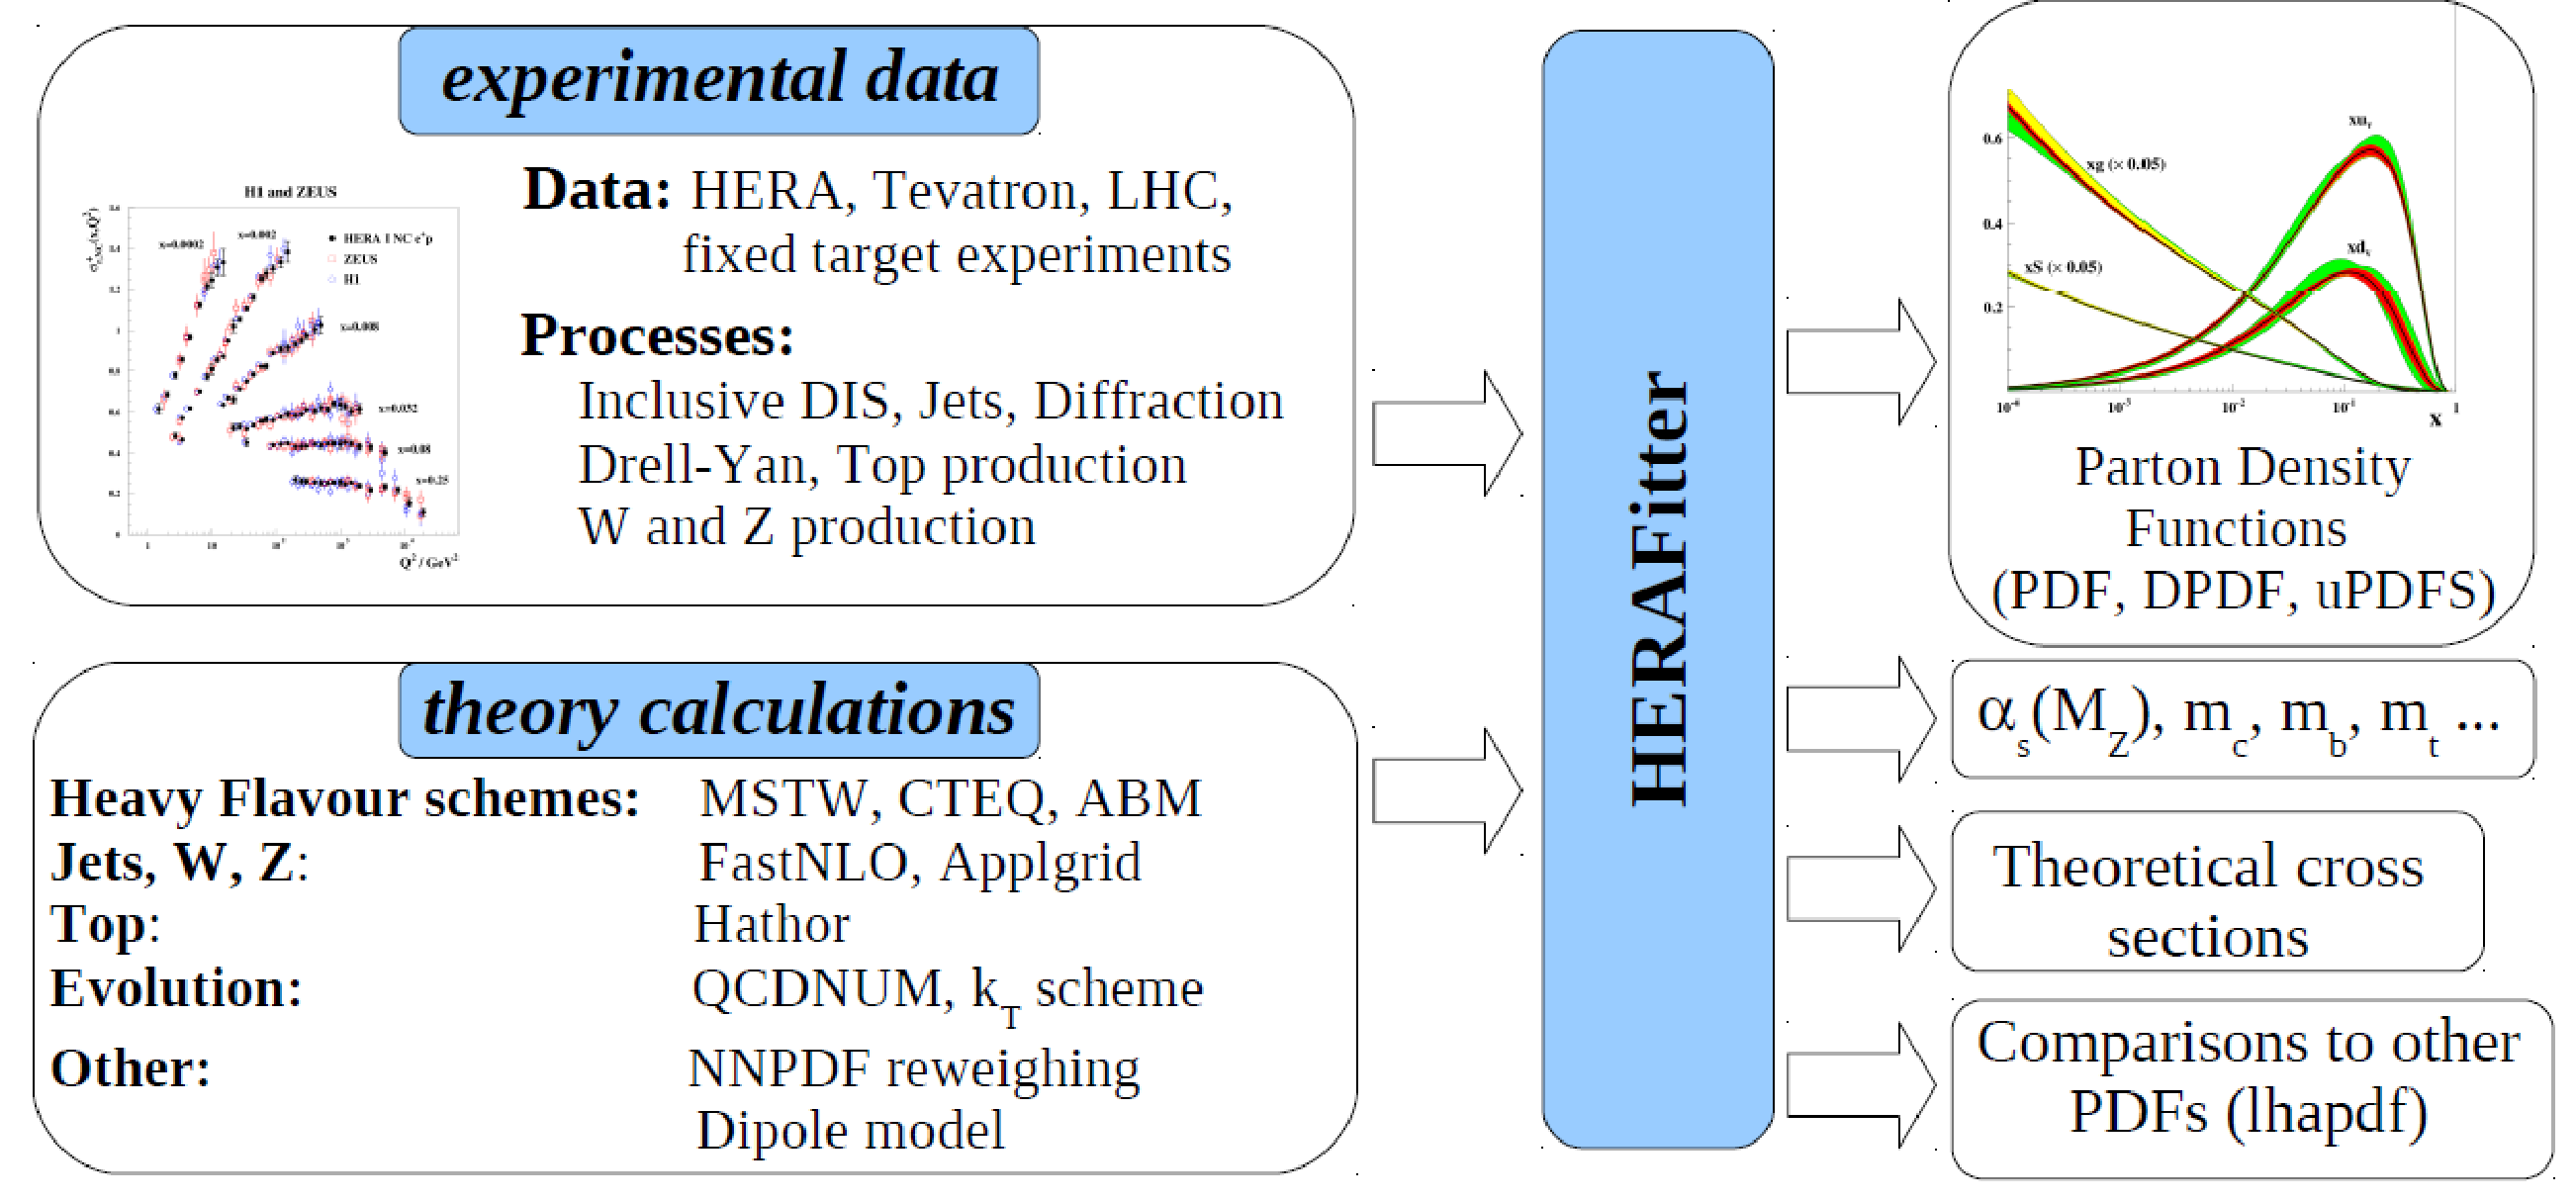
\includegraphics[width=0.75\linewidth]{figures/flow.pdf}
\caption{Schematic structure of the \fitter\ program.}
\end{center}
\label{fig:flow}
\end{figure}

The manual is structured such that it first describes briefly the
 theoretical input (section~\ref{sec:theory}), followed by a description of the
PDF parameterisation (section~\ref{sec:pdfparam}) and various $\chi^2$ functions used in the minimisation (section~\ref{sec:chi2}). The minimisation is based on the standard MINUIT program \cite{MINUIT} which is not discussed here.
Section~\ref{sec:progman} is dedicated to program installation instructions for different fit scenarios (section~\ref{sec:install}) and provides a description of the program steering cards with the output options given in section~\ref{sec:man}.
  
%%%%%%%%%%%%%%%%%%%%%%%%%%%%%%
\section{Theoretical Input}

\label{sec:theory}
\def\kt{\ensuremath{k_t}}
\newcommand{\Pmax}{p}
\newcommand{\CCFM}{CCFMa,CCFMb,Catani:1989sg,CCFMd}

The main features of QCD theory are confinement
(at short ranges the quarks are strongly bound inside protons)
and asymptotic freedom (at large scales the coupling constant 
of the strong force decreases and quarks become quasi-free partons).
The factorisation theorem exploits these features by 
separating short and long distances processes, such that 
structure functions can be written as a convolution 
between calculable parts (hard scattering coefficients) and 
non-calculable parts (parton distribution functions (PDFs)), 
which are therefore parametrised and determined from data.

Factorisation is most rigorously established for deep inelastic 
lepton-hadron scattering. For hadronic processes 
in which a colourless electroweak final state is produced (i.e. Higgs,
 a real or virtual $W$, $Z$ or~$\gamma$) factorisation is also well established
and differential cross section calculations are currently available up to 
next-to-next-to leading order (NNLO) in perturbation theory.

Factorisation is also proved to work for
sufficiently inclusive coloured final
states, such as the one-jet and dijet cross section.
In this case no fully rigorous all-order demonstration is 
available, but no counter-example to factorisation has been found so far.

For the diffractive case, two factorisations are used: the Regge factorisation
and the collinear factorisation for the hard scattering. 

The proton PDFs are classically extracted from QCD fits by a measure of 
the agreement between data and theory models.
The fit procedure used in the \fitter\ framework is common to all processes and it consists first 
in parametrising the PDFs at a starting scale  $Q^2_0$, chosen to be below the charm mass threshold. 
The PDFs are then evolved using coupled, integro-differential
Dokshitzer-Gribov-Lipatov-Altarelli-Parisi (DGLAP)~\cite{Gribov:1972ri,Gribov:1972rt,Lipatov:1974qm,
Dokshitzer:1977sg,Altarelli:1977zs} evolution equations 
as implemented in the QCDNUM~\cite{qcdnum} program in the $\overline{\text{MS}}$ scheme 
(LO, NLO nd NNLO evolutions are available~\cite{Curci:1980uw,Furmanski:1980cm}).
%The renormalisation and factorisation scales are set to $Q^2$. 
%(LO and NNLO evolutions are also available).
The PDFs calculated at a scale corresponding to a measured cross section are convoluted with the partonic 
cross sections to calculate the predicted cross section. For all measurement points, the predicted 
and measured cross sections together with their corresponding errors are used to build a global $\chi^2$, 
minimised to determine the initial PDF parameters. This generic procedure includes a number of 
subtleties and assumptions, depending on the measurements, scale and available calculations.

In the following sections, the theoretical input for various processes is described,
for example the electron-proton deep inelastic scattering (DIS) process in section 
\ref{dis}, the Drell-Yan process in section \ref{DY}. 
For the jet cross section calculations, \fitter\ uses  
APPLGRID or FastNLO, see section \ref{sec:theory:jets}.
In section \ref{ttbar} the $t\bar{t}$ cross sections are calculated based on the HATHOR package.
Alternative approaches to collinear factorisation
are also discussed, see sections \ref{dipole} for Dipole models and 
\ref{TMD} for unintegrated PDFs.
The diffractive PDFs are discussed in section \ref{diff},
in the context of the resolved Pomeron model which predicts
such processes as seminclusive diffractive scattering in DIS.

%%%%%%%%%%%
\subsection{Deep Inelastic Scattering Formalism and Schemes}
%There are different approaches to the treatment of the heavy quark production. 
%These include the fixed-flavour (FFN) and variable flavour number (VFN) schemes.
%%%%
\label{dis}

The DIS experiments provide the cleanest approach 
to measure the proton structure. 
The DIS experiments are carried out either on fixed targets 
or at collider facilities using electrons, muons or neutrinos 
to probe the proton. 
In the DIS process a lepton is scattered off the constituents of 
the proton by a virtual exchange of a neutral (NC) or charged (CC)
 boson producing a hadronic shower and a scattered lepton in the
final state. The DIS kinematic variables are illustrated 
in figure~\ref{fig:dis}:
the negative squared four-momentum of the exchange boson, $Q^2$, the 
scaling variable $x$, which can be related in the parton model to 
the fraction of momentum carried by the struck quark, and the 
inelasticity parameter $y$, which is the fraction of the energy 
transferred to the hadronic vertex. 
\begin{figure}
\begin{center}
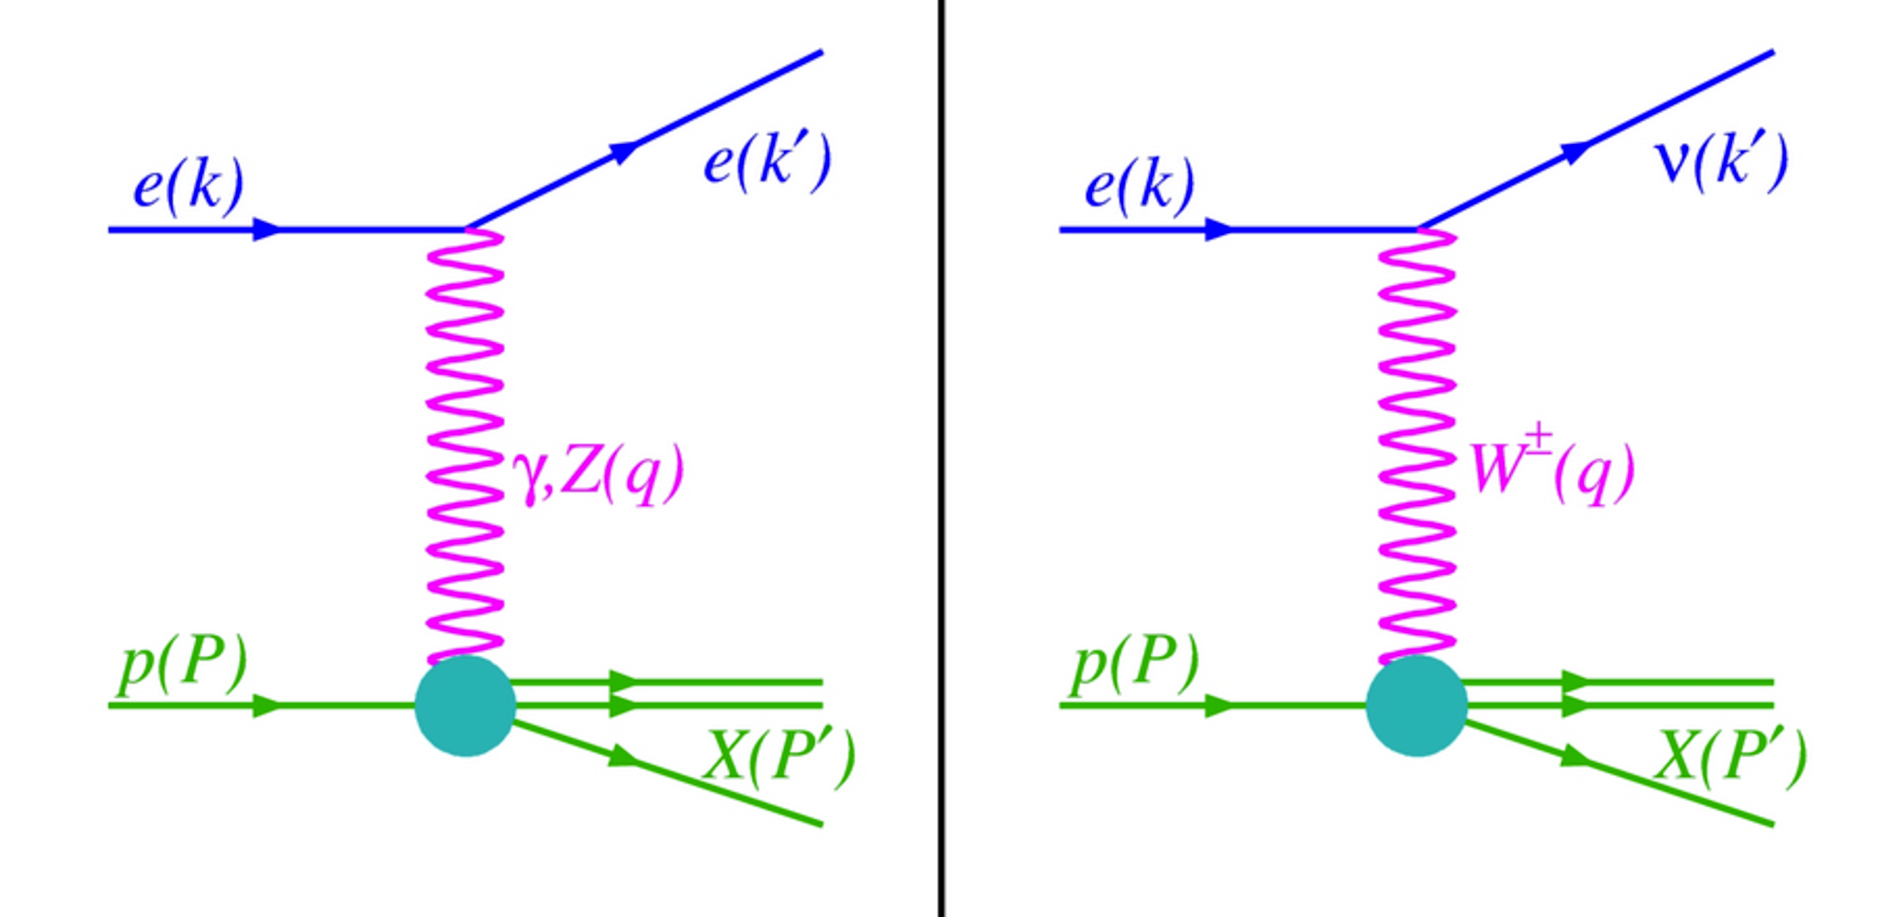
\includegraphics[width=0.5\linewidth]{figures/DIS.pdf}
\end{center}
\caption{Diagram for a neutral and charged current DIS scattering.}
\label{fig:dis}
\end{figure}
%
The NC (and similarly CC) cross section can be expressed in terms of generalised structure functions:
\begin{eqnarray}
   \frac{d^2\sigma_{NC}^{e^{\pm} p}}{dxdQ^2}=\frac{2\pi\alpha^2}{xQ^4} 
    \big [ Y_{+} \tilde F_2^{\pm} \mp Y_{-}x \tilde F_3^{\pm} - y^2 \tilde F_L^{\pm} \big ],
    %\label{eq:NC not reduced}
\end{eqnarray}
where $Y_{\pm} = 1 \pm (1-y)^2$. The structure function $\tilde F_2$
is the dominant contribution to the cross section, $x \tilde F_3$ is important at high $Q^2$ and $\tilde F_L$ is sizable
only at high $y$.
$\tilde F_2^{\pm}$ and $\tilde F_3^{\pm}$ can be expressed in terms of five structure
functions describing the contributions from pure photon exchange, $\gamma Z$ interference
and pure $Z$ exchange:  
% ------ F_2 ------------
\begin{center}
  \begin{eqnarray}
  \tilde F_2^{\pm} = F_2-v_e \Bigg( \frac{\kappa_W Q^2}{Q^2+M^2_Z} \Bigg)F_2^{\gamma Z}
   + (v_e^2 + a_e^2) \Bigg( \frac{\kappa_W Q^2}{Q^2+M^2_Z} \Bigg)^2 F_2^Z  \\ 
% ------ xF_3 ------------
  x\tilde F_3^{\pm} = \pm a_e \Bigg( \frac{\kappa_W Q^2}{Q^2+M^2_Z} \Bigg)xF_3^{\gamma Z}
  \mp 2a_e v_e \Bigg( \frac{\kappa_W Q^2}{Q^2+M^2_Z} \Bigg)^2 xF_3^Z   
 \end{eqnarray}
\end{center}
Here, the pure photon exchange is described by $F_2$, pure $Z$ exchange by $F_2^Z$ and
$xF_3^Z$, and $\gamma Z$ interference by $F_2^{\gamma Z}$ and $xF_3^{\gamma Z}$.
$v_e$ is the weak vector and $a_e$ the weak axial-vector coupling of the electron
to the $Z$. 
The Weinberg angle $\theta_W$ enters the quantity $\kappa_W$ in the following way: $\kappa_W = \frac{1}{4 \sin^2 \theta_W \cos^2 \theta_W}$.
\\ \\
%
In the framework of perturbative QCD the structure functions are directly related to the
parton distribution functions, i.e. in leading order (LO)  $F_2$ is the momentum sum of quark and anti-quark distributions
weighted by the quark charge squared:
\begin{center}
  \begin{eqnarray}
    \lbrack F_2,F_2^{\gamma Z},F_2^Z \rbrack =
   x \sum_q[e_q^2,2e_qv_q,v_q^2+a_q^2] \{ q(x,Q^2) + \overline q(x,Q^2) \} \\ 
   \lbrack xF_3^{\gamma Z},xF_3^Z \rbrack = 
   x \sum_q[e_q^2a_q,2v_qa_q]\{q(x,Q^2) - \overline q(x,Q^2)\}
 \end{eqnarray}
\end{center}
%$F_2 \approx x \sum e^2_q (q+ \overline q)$, and $xF_3$ is related to their difference,
%$xF_3 \approx x \sum 2e_q a_q (q- \overline q)$. At higher orders, terms related to the gluon density distribution
%($\alpha_s g$) appear.
%\\
In analogy to neutral currents, the inclusive CC $ep$ cross section can be expressed
in terms of structure functions:
\begin{center}
  \begin{equation}
   \frac{d^2\sigma_{CC}^{e^{\pm} p}}{dxdQ^2}=
   \frac{G_F^2}{4\pi x} \bigg( \frac{M_W^2}{Q^2+M_W^2} \bigg)^2
             \big [ Y_{+} W_2^{\pm} + y^2  W_L^{\pm} \mp Y_-x  W_3^{\pm} \big ],
  \label{eq:CC not reduced}
 \end{equation}
\end{center}
Here, $G_F$ is the Fermi constant which is related to the weak coupling $g$ and
electromagnetic coupling $e$, i.e. $G_F = \frac{g^2}{4 \sqrt{2} M_W^2}$.
%
In LO the $e^+p$ and $e^-p$ cross sections are sensitive to different quark flavours:
\begin{eqnarray}
  \begin{array}{rll}
    \tilde \sigma_{CC}^{e^{+} p} = 
    x[\overline u +\overline c] + (1-y)^2 x[ d+s ]  \\
    \tilde \sigma_{CC}^{e^{-} p} = 
    x[ u +c] + (1-y)^2 x[\overline d +\overline s ].
  \end{array}
\end{eqnarray}

The cross-section predictions are obtained by convoluting the PDFs with the 
hard scattering coefficient functions. 
There are various schemes for separating in 
%approaches of dividing 
the structure functions 
into calculable processes and PDFs.
For the DIS processes these are the Fixed-Flavour number 
(FFN)~\cite{Laenen:1992, Laenen:1993, Riem:1995} or the general mass 
Variable-Flavour number (GM-VFN)~\cite{VFN} schemes. 
%\fitter\ implements the zero mass variable flavour number (ZMVFN) scheme
% from QCDNUM and are discussed in the following subsections.
In the FFN scheme, heavy quark contributions are explicitly included in the hard cross sections. 
In the VFN scheme, PDFs corresponding to heavy quarks are introduced and the number of active 
flavors changes by one unit when the scale crosses the threshold for heavy quark distribution ($Q^2 \ge m_{Q}^2$).


%The various treatments for the heavy quark thresholds are implemented as provided by the MSTW group
The evolution program QCDNUM~\cite{qcdnum} used in \fitter\ provides 
the calculations of the deep inelastic structure functions in the zero-mass, 
generalised mass and the fixed flavour number schemes. 
VFN schemes with various treatments for the heavy 
quark  thresholds are considered in \fitter\ :
\begin{center}
 \begin{enumerate}
  \item[$\bullet$] the Thorne Roberts (TR) scheme with its variants at NLO and
  NNLO~\cite{Thorne:1997ga,Thorne:2006qt} as provided by the MSTW group,
  \item[$\bullet$] the ACOT scheme with its variants at LO and NLO as provided by the CTEQ group, 
  \item[$\bullet$]  BMSN scheme at NLO and NNLO~\footnote{The BMSN scheme as provided by the ABM group
      currently is not yet fully implemented in \fitter\ .}.
  \end{enumerate}
\end{center}  
The fixed-flavour number scheme
is available via the QCDNUM implementation and via the 
{\tt OPENQCDRAD}~\cite{openqcdrad:page} interface.
Each of these schemes is briefly discussed below.


\subsubsection{Zero-Mass Variable Flavour Scheme}

In the zero-mass variable flavour number scheme (ZM-VFNS) heavy quark densities are
included in the proton for $Q^2>>m_h^2$ but they are treated as massless in both
the initial and final states.
This scheme is accurate in the region where $Q^2$ is much greater than $m_h^2$
but becomes unreliable for $Q^2 \sim m_h^2$. 

%The un-polarised DIS structure functions in ZM-VFN scheme are computed as a 
%convolution of the parton densities with zero-mass coefficient functions and 
%in \fitter\ are activated via namelist {\tt HF$\_$SCHEME} in the {\tt steering.txt}.
%%%%
\subsubsection{General Mass Variable Flavour Scheme: Thorne-Roberts scheme}

The Thorne-Roberts (TR) scheme, (referred as RT scheme in the \fitter\ )
is a general-mass variable flavour number scheme (GM-VFNS)
 used as default for the MTSW PDF sets. GM-VFNSs smoothly connect the two regions: 
scales below ($Q^2<m_h^2$) and scales much above the heavy quark scale threshold ($Q^2>>m_h^2$). 
However, the connection is not unique.
A GM-VFNS can be defined by demanding equivalence of the $n_f = n$ (FFNS) 
and $n_f = n+1$ flavour (ZM-VFNS) descriptions above the transition point for the new parton distributions
(they are by definition identical below this point), at all orders.

The TR scheme has two different variants: TR standard (as used in MSTW PDF 
sets~\cite{Thorne:2006qt,Martin:epC63}) 
and TR optimal~\cite{Thorne:6180}, with a smoother transition across the heavy quark mass scales. 
Both of these variants are accessible within the \fitter\ package.
The calculations are available to NLO and NNLO. In addition, a fast version of the scheme 
is available (i.e. RT FAST) by using the k-factor technique. 
The k-factors are defined as the ratio between massless and massive scheme. 
They are applied to the fast massless scheme accessed by QCDNUM. 
However, the k-factors are only calculated correctly for the PDF parameters which enter the first 
iteration of the minimisation and are not updated with each iteration. 
Hence the RT-fast calculation must be repeated by inputting the final PDF parameters 
and iterating this procedure until the input and output PDFs are not significantly different
%The k-factors are applied at the first iteration of the minimisation process enabling the code to run fast, 
%as the k-factors are defined as the ratio between massless and massive scheme, while the massless scheme 
%accessed via QCDNUM is very fast.

 
%%%%
\subsubsection{General Mass Variable Flavour Scheme: ACOT scheme}

The Aivazis-Collins-Olness-Tung scheme belongs to the group of VFN 
factorisation schemes that use the renormalisation method of 
Collins-Wilczek-Zee (CWZ) \cite{CWZ}.
This scheme involves a mixture of the $\overline{\text{MS}}$ scheme 
for light partons (and for heavy partons when the factorisation scale 
is larger than the heavy quark mass) and the zero-momentum subtraction 
renormalisation scheme for graphs with heavy quark lines 
(if the factorisation scale is smaller than the mass of the heavy quark threshold). 
The DGLAP kernels and PDF evolution are pure  $\overline{\text{MS}}$.
% Definition of subtractions is analogous to  $\overline{\text{MS}}$. 
Therefore, the ACOT scheme is considered to be a minimal extension of the $\overline{\text{MS}}$ scheme.


Within the ACOT package, different variants of the ACOT scheme are available:
ACOT Full, S-ACOT Chi, ACOT ZM,  $\overline{\text{MS}}$  at LO and NLO. 
For the longitudinal structure function higher order
 calculations are also available. 
The ACOT Full implementation fully takes into account the quark masses and it reduces
to  $\overline{\text{MS}}$ scheme in the limit of masses going to zero, but it has the disadvantage 
of being quite slow.
Therefore the k-factor technique has been adopted within the \fitter\  
machinery in order to perform QCD fits. The k-factor can be defined in two different ways:
on the one hand as the ratio between same order calculations but massless vs massive 
(i.e. NLO (ZM-VFNS)/NLO (ACOT), on the other hand one could speed up the calculations by 
defining the k-factors as the ratio between LO (massless)/NLO (massive).
Both options are available in the \fitter\ package and give similar results. 
%k-factors depend on PDFs therefore same iterations of the fit are needed.
For convergence of the k-factors usually $2-3$ repetitions of the fit are needed.
The different variants of this scheme are all integrated in the \fitter\  framework and can be 
selected via the namelist {\tt HF$\_$SCHEME} in the {\tt steering.txt} (ACOT ZM, ACOT FULL, S-ACOT Chi).

The differences between TR and ACOT scheme types are summarised in the figure \ref{fig:schemes}.
One major issue in a complete GM-VFNS, is that of the ordering of the
perturbative expansion.
The equivalency of swapping the $O(m_{H}^2/Q^2)$ terms between Wilson coefficients (or hard-scattering amplitudes) 
without violating the definition of a GM-VFNS is what mainly distinguish the ACOT from TR schemes. 
\begin{figure}[!ht]
\begin{center}
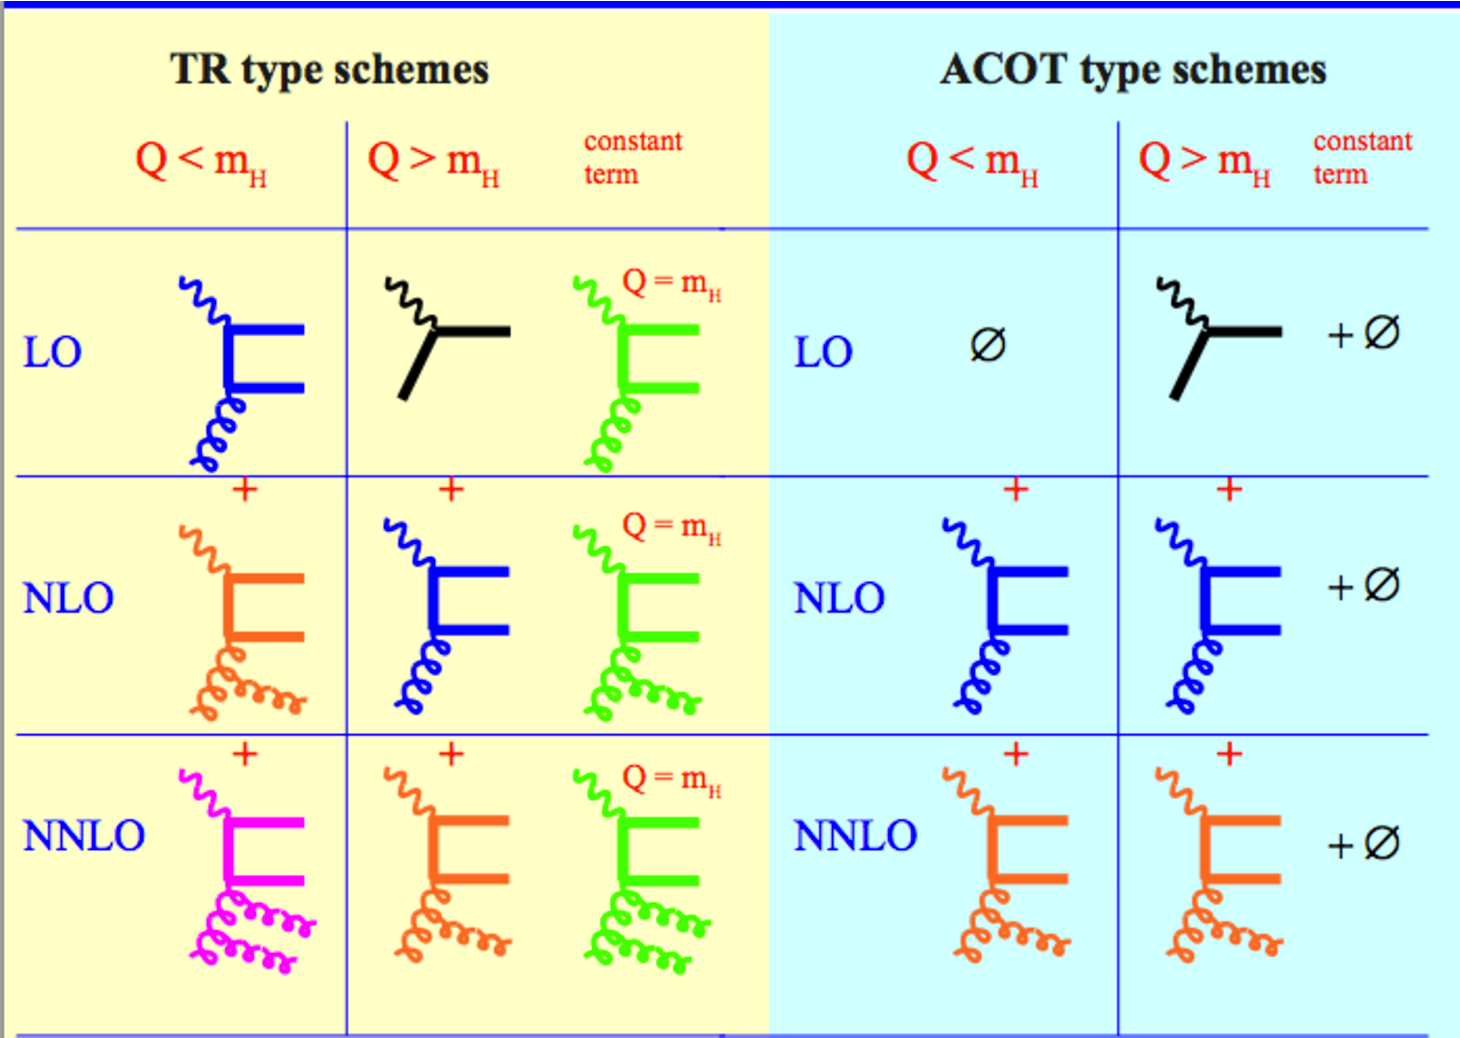
\includegraphics[width=0.5\linewidth]{figures/schemes.pdf}
\caption{Schematic summary of ACOT and TR schemes.}
\label{fig:schemes}
\end{center}
\end{figure}
%
%%%%
\subsubsection{Fixed -Flavour Number Scheme}

As mentioned before, in the FFN scheme only the gluon and the light quarks are considered
as partons within the proton, massive quarks are produced perturbatively in the final state.
\fitter\ includes the FFN scheme from ABM~\cite{openqcdrad:page} and can also use the QCDNUM implementation.
%The fixed-flavour number scheme for DIS structure functions in \fitter\ can be selected via {\tt HF$\_$SCHEME}
%using QCDNUM or ABM~\cite{openqcdrad:page} implementation.

In addition, a recent variation of the fixed-flavour number scheme in which the running mass definition
of the heavy quark mass is used in the $\overline{\text{MS}}$ scheme~\cite{Alekhin:runm} is implemented
in \fitter\ .This variant is realised via the interface to the open-source code 
OPENQCDRAD~\cite{openqcdrad:page}.
This scheme has the advantage of reducing the sensitivity of the DIS cross sections to
higher order corrections, and improving the theoretical precision of the mass definition. 
In QCDNUM, the calculation of the heavy quark contributions to DIS structure functions
are available at NLO and only electromagnetic exchange contributions are taken into account.
In the ABM implementation, the QCD corrections to the massive Wilson coefficients 
up to the currently best known approximate NNLO for the neutral-current (NC) 
heavy-quark production~\cite{SMoch:npb864} and up to NLO
for the charged-current (CC) case are available.
%
%The fixed-flavour number scheme for  in \fitter\ can be also accessed via interface to
%the open-source code OPENQCDRAD~\cite{openqcdrad:page} in \fitter\ framework 
%provides an access to 
%fixed flavour number scheme (FFNS)~\cite{Laenen:1992,Laenen:1993,Riem:1995}
%
%By default, in FFNS the number of light quark 
%flavours $n_{f}$ (here $n_{f}=3$) are considered in the PDF evolution and heavy (massive) 
%quarks appear only in the final state. 
%The QCD corrections to the massive Wilson coefficients which are known up to the NNLO
%for the neutral-current (NC) heavy-quark production~\cite{} are implemented in OPENQCDRAD.
%In the case of charged-current (CC), the massive NLO QCD corrections~\cite{} are available.
%In addition, the treatment of the heavy-quark contributions in DIS are provided 
%in both, the pole-mass and the running-mass definition in $\overline{\text{MS}}$ 
%scheme~\cite{Alekhin:runm}. \\
%In case the FFN scheme is chosen as the fitting option (see corresponding instructions in the section 1),
%the heavy quark contributions to DIS structure functions $F_2$ and $F_L$ (and $F_3$ in the charged 
%current case) are calculated in the FFNS and together with the light-flavor contributions are 
%provided for the theory prediction calculation (theory$\_$dispatcher.f).
%The interpolation to PDFs and $\alpha_s$ evolution from QCDNUM are set up in the interface to OPENQCDRAD. \\
%The variation of the renormalisation and factorisation scales for heavy quarks is 
%possible (see available options in steering.txt file).
%
%       
%%%%%%%%%%%
\subsubsection{Electroweak corrections for \texorpdfstring{$ep$}{ep} scattering} 
%%%%%%%%%%%
 
To properly compare the experimental data with theoretical predictions, 
QED corrections are necessary. In the \fitter\, the electroweak corrections 
for the DIS process are based on the EPRC package~\cite{SpiesbergerPrivComm}.
%provided by Hubert Spiesberger \cite{HS}.
%The measured cross sections as presented by HERA are not corrected for the weak corrections
%in order to retain sensitivity to higher order EW effects.

The calculations of higher-order electroweak corrections to DIS scattering at HERA are performed
in the on-shell scheme where the gauge bosons masses $M_W$ and $M_Z$ are treated symmetrically
as basic parameters together with the top and Higgs masses, besides the fine structure constant 
$\alpha$ and other fermion masses.

The code provides the running of $\alpha$ using the most recent parametrisation
of the hadronic contribution to $\Delta_\alpha$ \cite{Jegerlehner}, as well as an older 
one from Burkhard \cite{Burkhard}.
For the Drell Yan processes there are independent treatments applied as k-factors (such as 
from the SANC and FEWZ packages).

 


\subsection{Drell Yan processes}
%%%%
\label{DY}

This section presents calculations of Drell Yan processes that can be used to 
predict lepton pair production at the LHC or Tevatron.
The Drell-Yan process is shown in figure~\ref{fig:dy}. 
The calculations of the Drell Yan processes are known for many observables up to NNLO order.
For example, there are packages such as FEWZ~\cite{FEWZ} and DYNNLO~\cite{DYNNLO} for NNLO
or MCFM~\cite{MCFM} for NLO calculations. However, due to the complicated nature of these
calculation involving an increased number of diagrams with each additional order, these 
calculations are too slow to be used iteratively in a fit.
There are various methods to overcome this shortage: using the k-factors approximation 
from lower to higher order, or using the so-called grid technique 
(storing the matrix elements on grids such that the cross sections maybe calculated later by 
convoluting these grids with the input PDFs) when available.
\begin{figure}[!ht]
\begin{center}
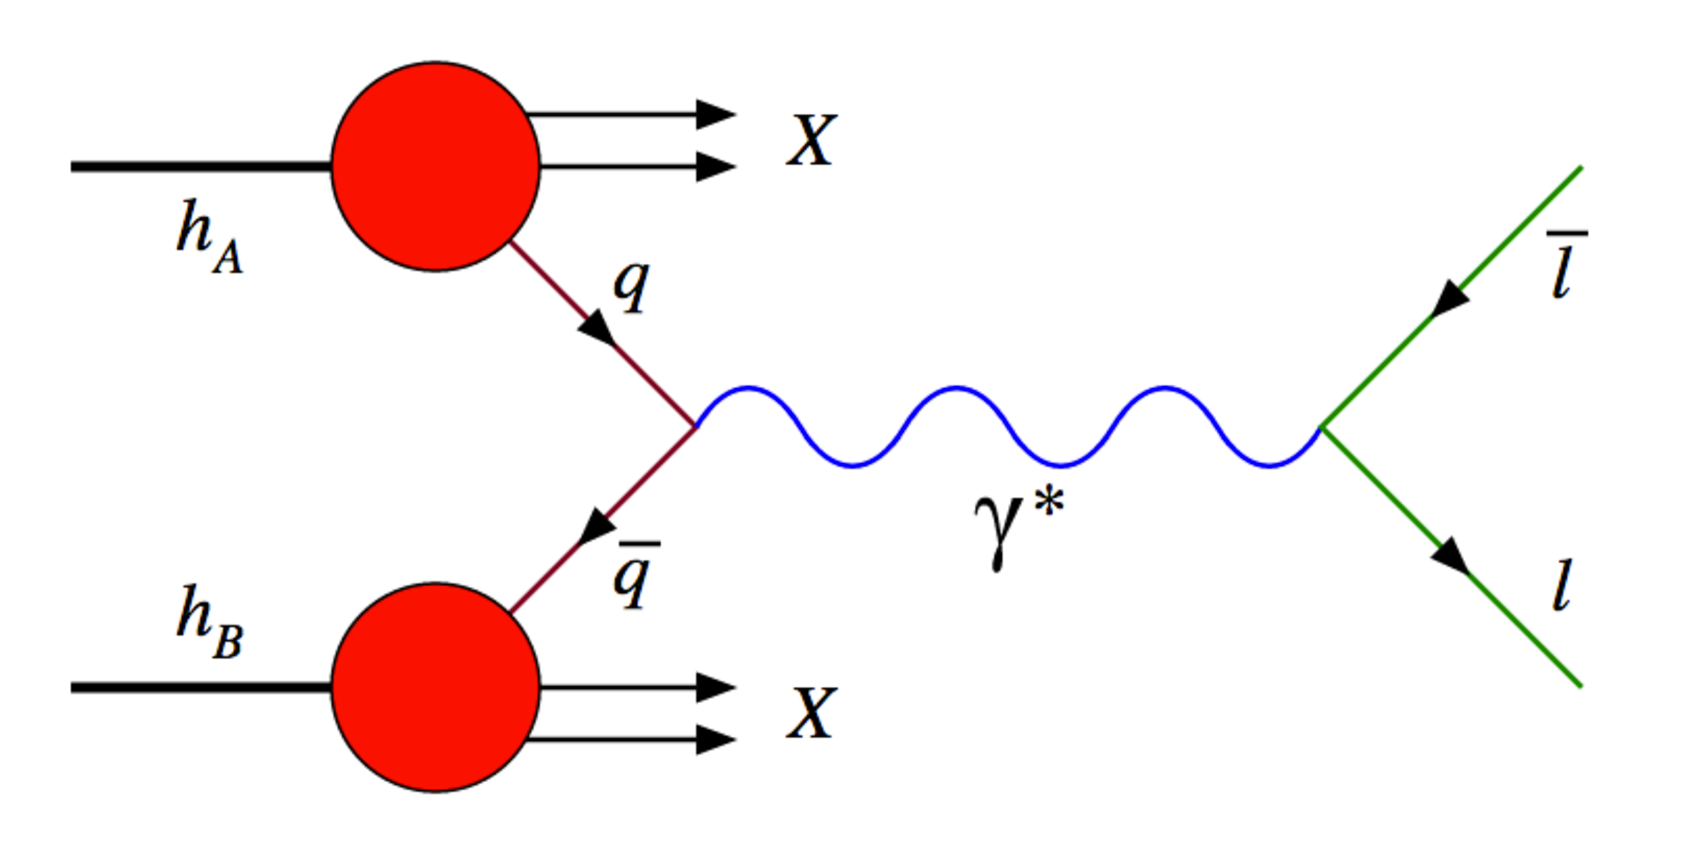
\includegraphics[width=0.5\linewidth]{figures/dy.pdf}
\end{center}
\caption{Diagram for a generic DY scattering.}
\label{fig:dy}
\end{figure}
  
\fitter\ provides two implementations for $pp$  Drell Yan processes.
The first implementation uses calculations at LO which can be extended to NLO using k-factors,
the second uses the APPLGRID interface. A short description of both implementations is 
given below while for details of the theoretical modules we direct the user the 
references for these packages provided in the description.
%
%For details of the theoretical modules we direct the user to read the provided references of these packages.


The leading order Drell-Yan~\cite{Drell:1970wh,Yamada:1981mw} 
triple differential cross section in
invariant mass \(M\), boson rapidity \(y\) and CMS
lepton scattering angle \(\cos\theta\),
for the neutral current, 
%triple differential in invariant mass \(M\), boson rapidity \(y\) and CMS
%lepton scattering angle \(\cos\theta\), 
can be written as
\begin{align}
\frac{\mathrm{d}^3\sigma}{\mathrm{d}M\mathrm{d}y\mathrm{d}\cos\theta} &=
  \frac{\pi\alpha^2}{3MS}\sum_{q}P_q
  \left[F_q(x_1,Q^2)F_{\bar{q}}(x_2,Q^2) + (q\leftrightarrow\bar{q})\right],
\end{align}
where \(S\) is the squared CMS beam energy, \(x_{1,2} = \frac{M}{\sqrt{S}}\exp(\pm y)\), $F_q(x_1,Q^2)$ parton distribution functions, and 
\begin{align}
  P_q &=  e_l^2e_q^2(1+\cos^2\theta) \nonumber \\
      &+  e_le_q\frac{2M^2(M^2-M_Z^2)}{\sin^2\theta_W\cos^2\theta_W
          \big[(M^2-M_Z^2)^2+\Gamma_Z^2M_Z^2\big]}
          \big[aA_q(1+\cos^2\theta)+2bB_q\cos\theta\big] \nonumber \\
      &+  \frac{M^4}{\sin^4\theta_W\cos^4\theta_W
          \big[(M^2-M_Z^2)^2+\Gamma_Z^2M_Z^2\big]}
          \big[(a^2+b^2)(A_q^2+B_q^2)(1+\cos^2\theta)+8abA_qB_q\cos\theta\big].
\end{align}
Here \(\theta_W\) is the Weinberg angle, \(M_Z\) and \(\Gamma_Z\) are Z boson mass and 
width, and
\begin{align}
 a & = -\frac{1}{4} + \sin^2\theta_W,  \nonumber \\
 b & = -\frac{1}{4},  \nonumber \\
 A_q & = \frac{1}{2}I_q^3-e_q\sin^2\theta_W, \nonumber \\
 B_q & = \frac{1}{2}I_q^3,  \nonumber \\
 I_u^3 & = -I_d^3 = \frac{1}{2},  \nonumber \\
 e_l & = -1, e_u = \frac{2}{3}, e_d = -\frac{1}{3}
\end{align}
give the electro-weak couplings.

The expression for charged current scattering has a simpler form.
\begin{align}
\frac{\mathrm{d}^3\sigma}{\mathrm{d}M\mathrm{d}y\mathrm{d}\cos\theta} &=
 \frac{\pi\alpha^2}{48S\sin^4\theta_W}
 \frac{M^3(1-\cos\theta)^2}{(M^2-M_W^2)+\Gamma_W^2M_W^2}
 \sum_{q_1,q_2}V_{q_1q_2}^2F_{q_1}(x_1,Q^2)F_{q_2}(x_2,Q^2),
\end{align}
where \(V_{q_1q_2}\) is the CKM quark mixing matrix and \(M_W\) and \(\Gamma_W\)
are \(W\) boson mass and decay width.

The simple form of these expressions allows the calculation of integrated
cross sections without utilisation of Monte-Carlo techniques.
This is particularly useful for PDF fitting purposes because
statistical fluctuations are avoided in this case. In both 
neutral and charged current expressions the parton density functions
factorise as functions dependent only on boson rapidity \(y\) and
invariant mass \(M\).
%leaving \(\cos\theta\) dependence aside.
The integral in \(\cos\theta\) can be computed analytically and
integrations in \(y\) and \(M\) can be performed with the Simpson
method. The \(\cos\theta\) parts are kept in the equation 
explicitly because their integration is asymmetric for
data in lepton \(\eta\) bins and also because of the need to apply 
lepton \(p_{\perp}\) cuts.

The fact that PDF functions factorise, allows high speed calculations when 
performing parameter fits over lepton rapidity data. In this case
the factorised part of the expression which is independent of PDFs can be
calculated only once for all minimisation iterations.
The leading order code in \fitter\ package implements this 
optimisation and uses fast convolution routines provided by
QCDNUM. Currently the full width LO calculations are optimised 
for lepton pseudorapidity and boson rapidity distributions with the
possibility to apply lepton \(p_{\perp}\) cuts.
%making this procedure flexible to describe data.
This flexibility allows the calculations to be performed within the phase space
corresponding to the available measurement.

%The calculated leading order cross sections are multiplied by
%NLO or NNLO k-factors provided for corresponding data distributions.
The calculated leading order cross sections are multiplied by
k-factors to obtain predictions at NLO or NNLO precision.
%%%%

Alternatively, one can obtain the NLO predictions directly by using 
APPLGRID or FASTNLO techniques, which rely on the factorisation theorem by 
decoupling the hard scattering coefficients from PDFs.
The hard scattering coefficients are calculated once and stored into a grid 
for a given kinematic bin, speeding up the convolution process with the PDFs 
and thus allowing to for fast QCD fits. 
These methods are described in more detail in section \ref{sec:theory:jets}

%%%%%%%%%%%
\subsection{Cross Sections for \texorpdfstring{$t\bar{t}$}{t-tbar} production in $pp$ or $p\bar p$ collisions}
\label{ttbar}
%This section presents the calculation tool available 
%in \fitter\ for top-guark pair prouction in $p \bar{p}$ and $pp$ collisions.
%
Top-quark pairs ($t\bar{t}$) are mainly produced at hadron colliders via $gg$ fusion and
$q \bar q$ annihilation. There are also $q q'$ and
$q g$ production modes.
The program HATHOR~\cite{Aliev:2010zk} allows the calculation of 
the expected total $t \bar t$ cross section at 
$p \bar p$ and $p p$ colliders up to approximate NNLO accuracy.
Version 1.3 of HATHOR includes the exact NNLO for $q \bar q \to t \bar t$ \cite{Baernreuther:2012ws}
as well as a new high-energy constraint on the approximate NNLO calculation obtained from
soft-gluon resummation \cite{Moch:2012mk}.
The default choice for renormalisation and factorisation scale in $t \bar t$ production is the top-quark mass, $m_t$.
The pole mass scheme is typically employed for $m_t$ but HATHOR also supports calculations in
the $\overline{\text{MS}}$ scheme.

\subsection{Jets}
\label{sec:theory:jets}
%In this subsection, the use of the factorisation formalism is fully exploited for the 
%calculations of the inclusive jets and dijet cross sections.
This sections presents various fast calculational techniques for jet production based on
the factorisation formalism.

The calculation of higher order jet cross sections is very demanding
in terms of computing power. The reasons are the large number of contributing
Feynman diagrams and also the large number of infrared divergences.
For an accurate cancellation of these singularities, the 
dipole subtraction method is often applied in such calculations.
During the necessary Monte Carlo integration a very fine phase
space sampling has to be performed in order to account for the
accurate cancellation of the counter terms.

In order to enable the inclusion of jet-cross section 
measurements in PDF and $\alpha_s$ fits, the perturbative
coefficients have to be pre-computed in a PDF and $\alpha_s$ 
independent way. For this purpose, two similar tools are
interfaced to the \fitter .

\subsubsection{FastNLO}
The fastNLO project~\cite{Kluge:2006xs,Wobisch:2011ij,Britzger:2012bs}
enables the inclusion of jet data in PDF and $\alpha_s$ fits.
This tool uses multi-dimensional interpolation
techniques to convert the convolutions of perturbative 
coefficients with parton distribution functions and 
the strong coupling into simple products.
%Although the concept is process independent, 
The perturbative 
coefficients are calculated by the \texttt{NLOJET++}
program~\cite{Nagy:1998bb} where calculations for jet-production
in DIS~\cite{Nagy:2001xb}  as well as in hadron-hadron 
collisions~\cite{Nagy:2003tz,Nagy:2001fj} with threshold-corrections 
of $\mathcal{O}$(NNLO) for inclusive jet cross 
sections~\cite{Kidonakis:2000gi} are available.

The fastNLO libraries are included in the \fitter\
package and no further requirements or compilation options
are needed. In order to include a new measurement into the PDF-fit,
the fastNLO tables have to be specified. These tables include all
necessary information about the perturbative coefficients and the
calculated process for all bins of a certain dataset. 
Tables for almost all published jet measurements
are available through the project website {\tt http://fastnlo.hepforge.org}.
%or have otherwise to be calculated by using the full fastNLO package.

Features of the fastNLO concept are the very quick convolution of the
perturbative coefficients with the PDFs, of
$\mathcal{O}(100 ms)$, and the very high accuracy
of the interpolation procedure. 
The fastNLO tables are conventionally calculated
for multiple factors of the factorisation scale, 
and the renormalisation scale factor can be chosen freely.
Some of the fastNLO tables already allow for 
%already involve a scale-independent
%concept~\cite{Britzger:2012bs}, which allows for 
the free choice~\cite{Britzger:2012bs} of the renormalisation and the factorisation
scale as a function of two pre-defined observables.
The evaluation of the strong coupling constant, which enters
the cross section calculation, is taken consistently from the 
QCDNUM evolution code.


\subsubsection{APPLGRID}
The APPLGRID~\cite{Carli:2010rw} package allows the fast computation 
of NLO cross sections for particular processes for arbitrary sets of 
proton parton density functions. The package implements
calculations of Drell Yan cross sections of electroweak boson (\(Z,W\))
production as well as jet production in proton-(anti)proton
collisions and DIS processes. 

The approach is based on storing the perturbative coefficients
of NLO QCD calculations of final-state observables measured
in hadron colliders in look-up tables. The PDFs and the 
strong couplings are included during the final calculations,
e.g. during PDF fitting. The method allows 
variation of factorisation and renormalisation scales in
calculations.

The look-up tables (grids) can be generated with modified versions
of MCFM~\cite{Campbell:1999ah,Campbell:2010ff} or 
NLOjet++~\cite{Nagy:2001fj} software as distributed
with the full version of APPLGRID package.
% NLO calculations
%for the current analysis are performed with the help of APPLGRID
%generated grids based on MCFM calculations. 

APPLGRID supports an interface to the MCFM parton level generators,
hence model input parameters such as electroweak parameters
are in fact pre-set following the MCFM input steering card, while
binning and definitions of the observables for which the
differential cross sections are needed are set in the 
APPLGRID code. 
%The grid parameters \(x_1, x_2\) and \(Q^2\) binning
The grid parameters, \(Q^2\) binning
and interpolation orders are also defined in the code.

APPLGRID constructs the grid tables in two 
steps: {\it (i)} exploration of the phase space in order
to optimize the memory storage and {\it (ii)} actual grid
construction in the phase space corresponding to the 
requested observables.

Afterwards the NLO cross sections are restored from the grids
using externally provided PDFs, \(\alpha_S\), factorization and 
renormalization scales. QCD NNLO k-factors can be applied
if requested.

In order to use APPLGRID tables in \fitter\ , the APPLGRID package 
has to be downloaded and installed first.
In addition, the \fitter\ code has to be configured with a special option 
(for details see section~\ref{sec:install}).
%Within \fitter\ package there are several APPGRID grid tables already 
%provided for the calculation of Drell Yan and jet processes which
%are data set specific.

%%%%%%%%%%%
\subsection{DIPOLE models}
\label{dipole}
%At low $x$ and low $Q^{2}$, virtual photon-proton scattering is described using the colour
%dipole model formalism~\cite{NNZ:91}. Within this formalism, the scattering process is calculated as a fluctuation of the
%photon into a quark-antiquark pair (dipole), with a lifetime $\propto\enskip 1/x$, which interacts with the proton.
%
%Several approaches have been developed to phenomenologically describe the dipole-proton interaction
%cross section, three of which are implemented in the fitter\. These are
%the original model version (GBW)~\cite{Golec-Biernat:1998js}, a model based on the colour glass condensate approach
%to the high parton density regime (IIM)~\cite{Iancu:2003ge}, and a modified GBW model by adding effects of the 
The dipole picture provides an alternative approach to the virtual photon-proton
 scattering at low $x$  because it allows the description of both inclusive and 
diffractive processes.
 In this approach, the virtual photon fluctuates into a $q\bar q$ (or $q\bar q g$) 
 dipole which interacts with the proton~\cite{NNZ:91}.  
The dipoles can be viewed as quasi-stable quantum mechanical states, which have very long 
life time $\propto 1/m_p x\;$ and a size which is not changed by scattering.
A schematic view of dipole factorisation at small $x$ in DIS is illustrated in figure~\ref{fig:dipole}.
The virtual photon fluctuates into a quark-antiquark pair and subsequently interacts with the target, 
and the dynamics of the interaction are embedded in the dipole scattering amplitude.

\begin{figure}
\begin{center}
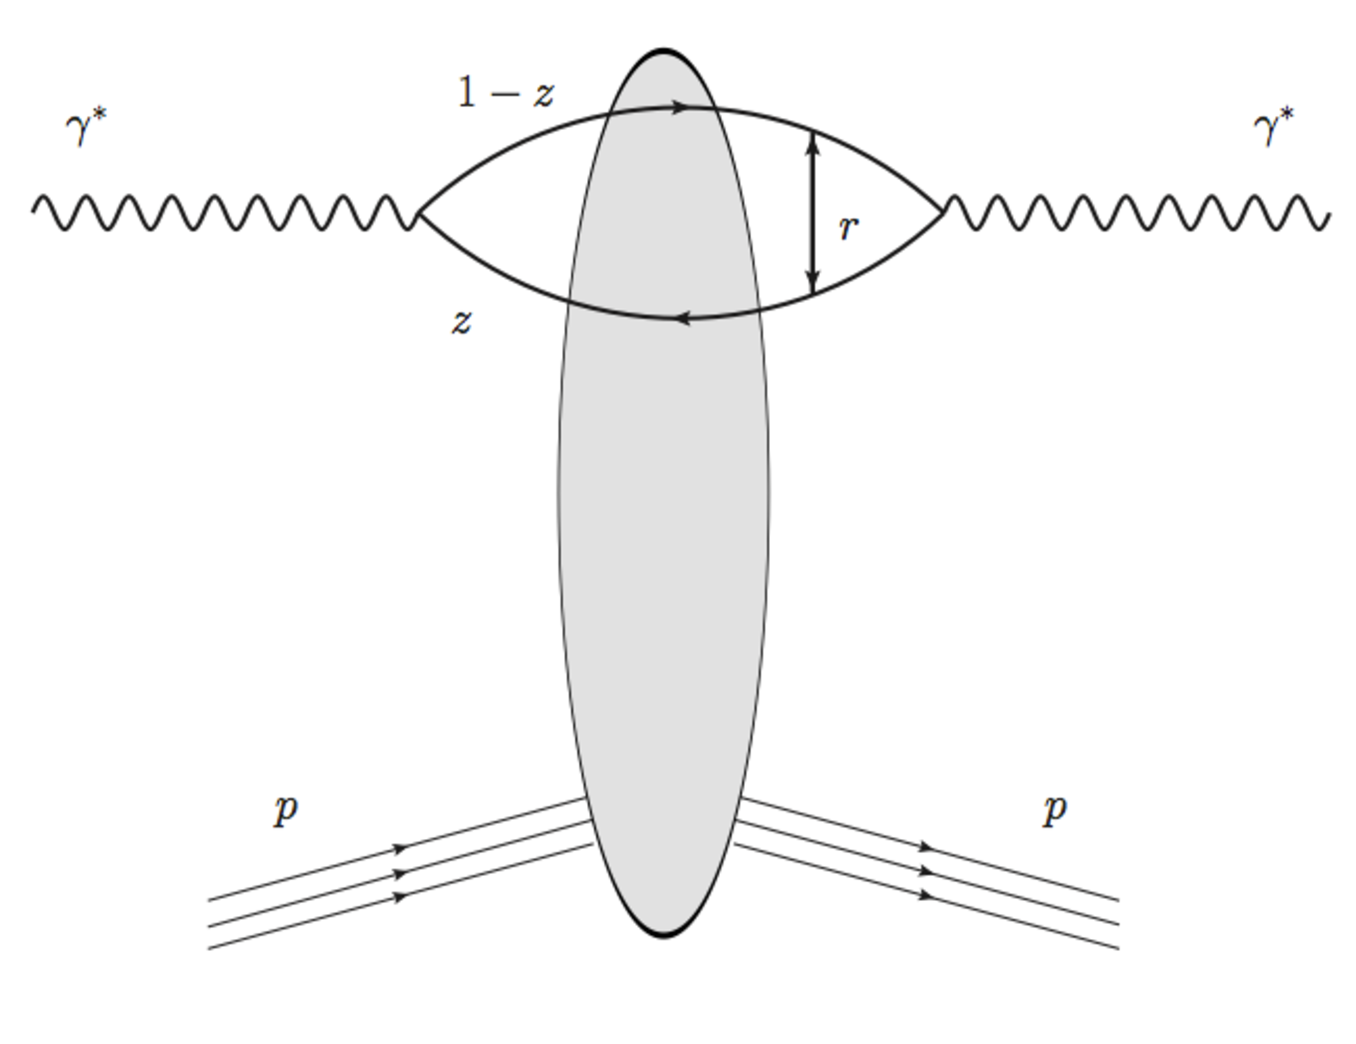
\includegraphics[width=0.5\linewidth]{figures/dipole.pdf}
\end{center}
\caption{Schematic diagram of dipole factorisation for the inclusive cross section in DIS.}
\label{fig:dipole}
\end{figure}

Several dipole models have been developed to describe various DIS reactions. 
They vary due to different assumption made about the behavior of the dipole-proton cross sections.   
In the \fitter\  three representative models  are implemented:
%\begin{itemize}
%\item the original Golec-Biernat-W\"usthoff (GBW)~\cite{Golec-Biernat:1998js} 
the original Golec-Biernat-W\"usthoff (GBW)~\cite{Golec-Biernat:1998js} 
dipole saturation model,
the colour glass condensate approach to the high parton density 
regime Iancu-Itakura-Munier (IIM) model~\cite{Iancu:2003ge} and 
a modified GBW model which takes into account the effects of  
DGLAP evolution Bartels-Golec-Kowalski(BGK)~\cite{Bartels:2002cj}.
%\end{itemize}
%%%%
\subsubsection{GBW model}

In the GBW model the dipole-proton cross section $\sigma_{\text{dip}}$ is given by
\begin{equation}
\label{eGBW}
   \sigma_{\text{dip}}(x,r^{2}) = \sigma_{0} \left(1 - \exp \left[-\frac{r^{2}}{4R_{0}^{2}(x)} \right]\right),
\end{equation}
where $r$ corresponds to the transverse separation between the quark and the antiquark, and $R_{0}^{2}$
 is 
%an $x$ dependent scale parameter, having the form $R_{0}^{2}(x)=\left(x/x_{0}\right)^{\lambda}$.
an $x$ dependent scale parameter which has corresponds to a saturation radius,  $R_{0}^{2}(x)=\left(x/x_{0}\right)^{\lambda}$.
The free fitted parameters are the cross-section normalisation $\sigma_{0}$ as well as $x_{0}$ and $\lambda$.
%%%%
\subsubsection{IIM model}
The IIM model assumes an improved expression for the dipole cross section which is based on the 
Balitsky-Kovchegov equation~\cite{Balitsky:1995ub}. The explicit formula for $\sigma_{\text{dip}}$ 
can be found in~\cite{Iancu:2003ge}. The free fitted parameters are an alternative scale parameter $\tilde{R}$, $x_{0}$ and $\lambda$.
%%%%
\subsubsection{BGK model}
The BGK model modifies the GBW model by taking into account the  DGLAP evolution
of the gluon density. 
The dipole cross section is given by
\begin{equation*}
\label{eBGK}
   \sigma_{\text{dip}}(x,r^{2}) = \sigma_{0} 
\left(1 - \exp \left[-\frac{\pi^{2} r^{2} \alpha_{s}(\mu^{2}) xg(x,\mu^{2})}{3 \sigma_{0}} \right]\right).
\end{equation*}
The factorization scale $\mu^{2}$ has the form $\mu^{2} = C_{bgk}/r^{2}+\mu^{2}_{0}$.
%This model uses the following gluon density at the starting scale $Q_{0}^{2}=1\mbox{ GeV}^{2}$
In this model the gluon density, which  is parametrized  at some starting scale $Q_{0}^{2}$ by
\begin{equation*}
\label{eqTH730}
   xg(x,Q^{2}_{0}) = A_{g} x^{-\lambda_{g}}(1-x)^{C_{g}}.
\end{equation*}
is evolved to larger $Q^2$'s using LO and NLO DGLAP evolution.
The free fitted parameters for this model are $\sigma_{0}$, $\mu^{2}_{0}$ and three parameters for the gluon density: $A_{g}$, $\lambda_{g}$, $C_{g}$. The parameter $C_{bgk}$ is kept fixed: $C_{bgk} = 4.0$. 
%%%%
%\newpage
%\subsubsection{Mixed with DGLAP model}
\subsubsection{BGK model with valence quarks}

The dipole models are valid in the low-$x$ region only, where the valence quark contribution is small, of the order of 5\%. The new HERA $F_2$ data have a precision which is  better than 2 \%. Therefore, in the \fitter\ the contribution of the valence quarks is taken from the PDF fits and added to the original 
 BGK model, this is uniquely possible within the \fitter\ framework.
 The quality of the fits of the BGK dipole model with valence quarks and without 
valence quarks are the same. The sample input steering and output fits are discussed in section~\ref{sec:man}.



%%%%%%%%%%%
%\subsection{Unintegrated PDFs using CASCADE}
\subsection{Transverse Momentum Dependent (unintegrated PDF) with CCFM}
\label{TMD}
In this subsection another alternative approach to the collinear DGLAP evolution is presented.
In high energy factorization \cite{Catani:1990eg} generally the measured cross section is written
 as a convolution of the partonic cross section $\hat{\sigma}(� \kt)$ which depends on the transverse 
momentum $\kt$ of the incoming parton with the $\kt$-dependent parton density function 
${\cal \tilde A}\left(x,\kt,\Pmax\right)$ (transverse momentum dependent (TMD) or unintegrated uPDF):
\begin{equation}
 \sigma  = \int 
\frac{dz}{z} d^2k_t \hat{\sigma}(\frac{x}{z},k_t)  {\cal \tilde A}\left(x,\kt,\Pmax\right)
\label{kt-factorisation}
\end{equation}
The evolution of ${\cal \tilde A}\left(x,\kt,\Pmax\right)$ 
can proceed via the BFKL, DGLAP or via the CCFM evolution equations.
 Here, an extension of the CCFM \cite{\CCFM} evolution is applied. 
Since the evolution cannot be easily obtained in  a closed form, 
 first a kernel $ {\cal \tilde A}\left(x'',\kt,\Pmax\right) $ 
is determined from the MC solution of the CCFM evolution equation, 
and then is then folded with the non-perturbative starting distribution 
${\cal A}_0 (x)$~\cite{Jung:2012hy}:
\begin{eqnarray}
x {\cal A}(x,\kt,\Pmax) &= &x\int dx' \int dx'' {\cal A}_0 (x) {\cal \tilde A}\left(x'',\kt,\Pmax\right)  \delta(x' \cdot x'' - x) \\
&= &\int dx' \int dx'' {\cal A}_0 (x) {\cal \tilde A}\left(x'',\kt,\Pmax\right) \frac{x}{x'} \delta(x'' - \frac{x}{x'}) \\
& = & \int dx' {{\cal A}_0 (x') }  
\cdot \frac{x}{x'}{ {\cal \tilde A}\left(\frac{x}{x'},\kt,\Pmax\right) } 
\end{eqnarray}
%An intrinsic $\kt$ dependence is included in the kernel ${\cal \tilde A}$
%\begin{eqnarray}
%{\cal \tilde A} & = & {\cal \tilde A'} \cdot f(k_{t\;0}) = {\cal \tilde A'} \cdot  \exp\left[ 
%-\frac{(\mu-k_{t\;0})^2}{\sigma^2}\right]
%\end{eqnarray}
The kernel  ${\cal \tilde A}$ includes all the dynamics of the evolution,
 Sudakov form factors and splitting functions and is determined in 
a grid of $50\otimes50\otimes50$ bins in $x,\kt,\Pmax$.  

The calculation of the cross section according to Eq.(\ref{kt-factorisation})
 involves a multidimensional Monte Carlo integration which is time consuming
 and suffers from numerical fluctuations, and therefore cannot be used directly in a fit
 procedure involving the calculation of numerical derivatives in the search for the minimum. 
Instead the following procedure is applied:
\begin{eqnarray}
\sigma_r(x,Q^2) & = & \int_x^1 d x_g {\cal A}(x_g,\kt,\Pmax) \hat{ \sigma}(x,x_g,Q^2) \\
  & = & \int_x^1 dx' {\cal A}_0 (x') \cdot \tilde{ \sigma}(x/x',Q^2) \label{final-convolution}
 \end{eqnarray}

The kernel ${\cal \tilde A}$ has to be provided separately and is not
 calculable within this program. The starting distribution  ${\cal A}_0$ 
 at the starting scale $Q_0$ of the following form is used:
\begin{eqnarray}
x{\cal A}_0(x,\kt) &=& N x^{-B_g} \cdot (1 -x)^{C_g}\left( 1 -D_g x\right) 
\label{a0}
\end{eqnarray}
with free parameters $N,\, B_g,\, C_g,\, D_g$. 
%In the present version, only the transverse momentum dependent gluon distribution 
%can be obtained from the fit. 

The calculation of the $ep$ cross section follows eq.(\ref{kt-factorisation}), 
with the off-shell matrix element including quarks masses taken from \cite{Catani:1990eg} 
in its implementation in {\tt CASCADE} \cite{Jung:2010si}.
In addition to the boson gluon fusion process, also valence quark initiated 
$\gamma q\to q$ processes are included, with the valence quarks taken from~\cite{Deak:2010gk}.
%Please note that in the present version only DIS $ep$ processes can be used
% to determine the transverse momentum dependent (uPDF) gluon density distribution.

%%%%%%%%%%%
\subsection{Diffractive PDFs}
\label{diff}
\newcommand{\asotp}{\ensuremath{\frac{\alpha_{\rm s}}{2\pi}}}
\newcommand{\Sgl}[1]{\ensuremath{\tilde f_{#1+}}}
\newcommand{\Pom}{{I\!P}}
\newcommand{\Reg}{{I\!R}}

In this section the diffractive process is briefly described.
It was observed at HERA that about 10\%
of deep inelastic interactions are diffractive leading to
events in which the interacting proton stays intact ($ep\to eXp$). 
In the diffractive process the proton appears well separated from the 
rest of the hadronic final state by a large rapidity gap, otherwise
the events look similar to normal deep inelastic events.
This process is usually  interpreted as the diffractive dissociation 
of the exchanged virtual photon to produce any hadronic final state
system $X$ with mass much smaller than $W$ and the same net quantum numbers as the exchanged photon.
Figure~\ref{fig:diff} illustrates the kinematic variables used to describe
 the inclusive diffractive DIS process.  For this, the 
proton vertex factorisation approach
is assumed such that  the diffractive DIS is mediated by the exchange of hard Pomeron and a
 secondary Reggeon.  The factorisable pomeron picture has proved remarkably successful for the description of most of these data.


\begin{figure}[!ht]
\begin{center}
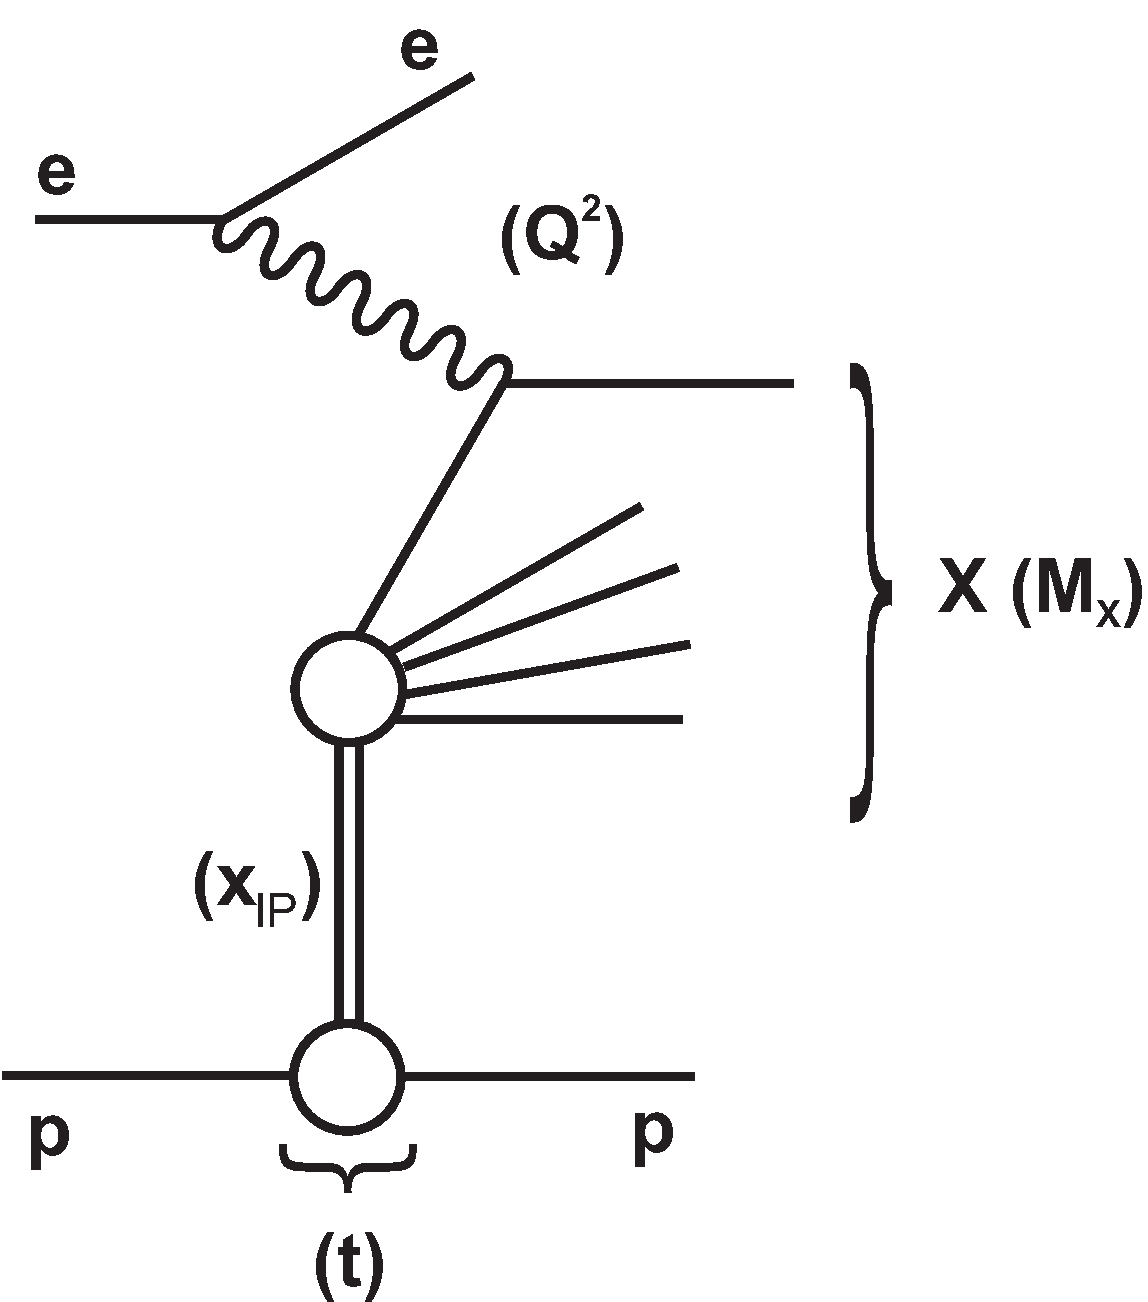
\includegraphics[width=0.5\linewidth]{figures/diffraction.pdf}
\end{center}
\caption{Schematic diagram of the kinematic variables used to
 describe the inclusive diffractive DIS process.}
\label{fig:diff}
\end{figure}

 In addition to $x$, $Q^2$ and the squared four-momentum transfer $t$
(the undetected momentum transfer to the proton system),
the mass $M_X$ of the diffractively produced final state provides
 a further degree of freedom. In practice, the variable $M_X$ is often replaced by $\beta$,
\begin{equation}
\beta=\frac{Q^2}{M_X^2+Q^2-t}.
\end{equation}

In models based on a factorisable pomeron, $\beta$ may be viewed as the fraction of the
pomeron longitudinal momentum which is carried by the struck parton, $x=\beta\Pom$.
%The diffractive parton distribution functions (DPDFs) are interpreted as probabilities for 
%finding a parton with a small fraction of the proton momentum $x=\beta\Pom$

\subsubsection {Cross-section}

As for the inclusive case, the diffractive cross-section can be expressed as:
\begin{equation}
  \frac{d\sigma}{d\beta\,dQ^2d\xi\,dt}
=
  \frac{2\pi\alpha^2}{\beta Q^4}\,
    \left( 1 +  (1-y)^2 \right) \ensuremath{\overline\sigma}^{D(4)}(\beta,Q^2,\xi,t)
\label{Dxs}
\end{equation}
where the ``reduced cross-section'' , $\overline\sigma$, is defined as
\begin{equation}
\overline\sigma^{D(4)}
 = F_2^{D(4)} - \frac{y^2}{1 +  (1-y)^2}\, F_L^{D(4)}
 = F_T^{D(4)} + \frac{2(1-y)}{1 +  (1-y)^2}\, F_L^{D(4)}
\label{eq:sigred}
\end{equation}
The dimension of $F_k^{D(4)}(\beta,Q^2,\xi,t)$
is $GeV^{-2}$ and thus the quantities integrated over $t$.
\begin{equation}
F_k^{D(3)}(\beta,Q^2,\xi)
\equiv
\int_{t_{\rm min}}^{t_{\rm max}} dt
F_k^{D(4)}(\beta,Q^2,\xi,t)
\end{equation}
are dimensionless. Maximum kinematically allowed value of $t$ reads as
\begin{equation}
t_{\rm MAX} 
=
-\frac{\xi^2 m_p^2 + p_\perp^2}{1-\xi}
\approx 
-\frac{\xi^2}{1-\xi} m_p^2
\end{equation}
where $m_p$ is the proton mass.
As $x = \xi\beta$ we can normalize to the standard DIS formula
\begin{equation}
\frac{d\sigma}{d\beta\,dQ^2\,d\xi\,dt} =
  \frac{2\pi\alpha^2}{x\, Q^4}\,
    \left( 1 +  (1-y)^2 \right) \xi\ensuremath{\overline\sigma}^{D(4)}(\beta,Q^2,\xi,t)
\end{equation}
which upon integration over $t$ reads
\begin{equation}
\label{Dxs3}
  \frac{d\sigma}{d\beta\,dQ^2\,d\xi}
=  
  \frac{2\pi\alpha^2}{x Q^4}\,
    \left( 1 +  (1-y)^2 \right) \,\xi\ensuremath{\overline\sigma}^{D(3)}(\beta,Q^2,\xi).
\end{equation}
%The H1 and ZEUS data files typically contain $\xi\ensuremath{\overline\sigma}^{D(3)}$.
The diffractive structure functions can be expressed as convolutions of the
calculable coefficient functions with diffractive quark and gluon distribution functions,
 which in general depend on all of $x$, $Q^2$, $\beta$, $t$.


%==========================================
\subsubsection {Regge factorization}
For a  better description of data, a contribution from a secondary Reggeon, $\Reg$, is included, hence
\begin{equation}
F_k^{D(4)}(\beta,Q^2,\xi,t) = 
\sum_{\mathcal{X} =\Pom,\Reg}
\phi_\mathcal{X}(\xi,t)\, F^\mathcal{X}_k(\beta,Q^2)
\end{equation}
or
\begin{equation}
\label{eq:FD3}
F_k^{D(3)}(\beta,Q^2,\xi) = 
\sum_{\mathcal{X} =\Pom,\Reg}
\Phi_\mathcal{X}(\xi)\, F^\mathcal{X}_k(\beta,Q^2)
\end{equation}
where
\begin{equation}
\label{eq:intFlux}
\Phi_{\mathcal{X}}(\xi) =
\int\limits_{t_{\rm min}}^{t_{\rm max}} dt\, \phi_\mathcal{X}(\xi,t)
\,.
\end{equation}
Parametrization of the fluxes follows
\begin{subequations}
\label{eq:flux}
\begin{equation}
\phi_\mathcal{X}(\xi,t) = 
\frac {A_\mathcal{X}\, e^{b_\mathcal{X} t}} {\xi^{2\alpha_\mathcal{X}(t) -1}}
\end{equation}
where
\begin{equation}
\alpha_\mathcal{X}(t) = \alpha_\mathcal{X}(0) + \alpha_\mathcal{X}' t
\,.
\end{equation}
\end{subequations}
$F^\Reg_k(\beta,Q^2)$ are taken as those of the pion.
%  with the normalization factor being absorbed in $\phi_\Reg(\xi,t)$.

%\newcommand\Version{2.01.02}
\newif\ifFullVer\FullVertrue
\FullVerfalse

% \texorpdfstring

\renewcommand\topfraction{0.5}
\renewcommand\bottomfraction{0.5}
\renewcommand\textfraction{0.5}
\renewcommand\floatpagefraction{0.5}

\makeatletter
\def\comsp{\@ifnextchar,\relax{\@ifnextchar\ \relax{\@ifnextchar:\relax{\@ifnextchar.\relax\ }}}}
\makeatother
\DeclareRobustCommand{\ie}{{\it i.e.}\comsp}
\DeclareRobustCommand{\eg}{{\it e.g.}\comsp}
\DeclareRobustCommand{\cf}{{\it cf.}\comsp}
\DeclareRobustCommand{\etal}{{\it et al.}\comsp}
\DeclareRobustCommand\bs{\ensuremath{\backslash}}
\newcommand\ssp{\ifmmode\relax\else\comsp\fi}

%\newcommand\Eq[1]{Eq.~(\ref{#1})}
\newcommand\Eq[1]{(\ref{#1})}
\newcommand\Fig[1]{Fig.~\ref{#1}}
\DeclareRobustCommand\NF{\ensuremath{N_{\rm f}}\ssp}
% \DeclareRobustCommand\NC{\ensuremath{N_{\rm c}}\ssp}
\DeclareRobustCommand\GeV{\ensuremath{{\rm GeV}}\ssp}
% \DeclareRobustCommand\Vstat{\ensuremath{V^{\rm (stat)}}\ssp}
% \DeclareRobustCommand\Vsys{\ensuremath{V^{\rm (sys)}}\ssp}
\DeclareRobustCommand\FL{\ensuremath{F_{\mathrm{L}}}\ssp}
\DeclareRobustCommand\FT{\ensuremath{F_{\mathrm{T}}}\ssp}
\newcommand\AP {{\cal P}}

\def \beq{\begin{equation}}
\def \eeq{\end{equation}}
\def \beqa{\begin{eqnarray}}
\def \eeqa{\end{eqnarray}}
\def \beqal{\begin{subequations}\begin{eqnarray}}
\def \eeqal{\end{eqnarray}\end{subequations}}

\let\optspace=\ssp
% \newcommand{\xh}{\hat x}
\DeclareRobustCommand{\as}[1]{\ensuremath{\alpha_{\rm s}(#1^2)}\optspace}
\newcommand{\asotp}{\ensuremath{\frac{\alpha_{\rm s}}{2\pi}}\optspace}
\newcommand{\Sgl}[1]{\ensuremath{\tilde f_{#1+}}\optspace}
\newcommand{\Pom}{{I\!P}}
\newcommand{\Reg}{{I\!R}}
% \newcommand{\xP}{x_\Pom}
\newcommand{\xP}{\xi}
\newcommand\sigRed{\ensuremath{\overline\sigma}}
\newcommand\DX{\ensuremath{\mathcal{X}}}

%\parindent=0pt
%\parskip=4pt

%\graphicspath{{figs/}}

%==========================================
\subsubsection {Cross-section}

\beq
  \frac{d\sigma}{d\beta\,dQ^2\,d\xP\,dt}
=
  \frac{2\pi\alpha^2}{\beta Q^4}\,
    \left( 1 +  (1-y)^2 \right) \sigRed^{D(4)}(\beta,Q^2,\xP,t)
\label{Dxs}
\eeq
where the `reduced cross-section', \sigRed, is defined as
\beq
\label{eq:sigred}
\sigRed
 = F_2 - \frac{y^2}{1 +  (1-y)^2}\, \FL
 = \FT + \frac{2(1-y)}{1 +  (1-y)^2}\, \FL
\eeq
Nb. $\xi$ is denoted by $x_\Pom$ in the H1 and ZEUS papers.

The dimension of 
\(
F_k^{D(4)}(\beta,Q^2,\xP,t)\)
is $\GeV^{-2}$
and
thus the quantities integrated over $t$
\beq
F_k^{D(3)}(\beta,Q^2,\xP)
\equiv
\int_{t_{\rm min}}^{t_{\rm max}} dt
F_k^{D(4)}(\beta,Q^2,\xP,t)
\eeq
are dimensionless.

Maximum kinematically allowed value of $t$ reads
\begin{equation}
t_{\rm MAX} 
=
-\frac{\xP^2 m_p^2 + p_\perp^2}{1-\xP}
\approx 
-\frac{\xP^2}{1-\xP} m_p^2
\end{equation}
where $m_p$ is the proton mass.

As $x = \xP\beta$ we can normalize to the standard DIS formula
\begin{equation}
\frac{d\sigma}{d\beta\,dQ^2\,d\xP\,dt} =
  \frac{2\pi\alpha^2}{x\, Q^4}\,
    \left( 1 +  (1-y)^2 \right) \xP\sigRed^{D(4)}(\beta,Q^2,\xP,t)
\end{equation}
which upon integration over $t$ reads
\begin{equation}
\label{Dxs3}
  \frac{d\sigma}{d\beta\,dQ^2\,d\xP}
=  
  \frac{2\pi\alpha^2}{x Q^4}\,
    \left( 1 +  (1-y)^2 \right) \,\xi\sigRed^{D(3)}(\beta,Q^2,\xP)
\end{equation}


The H1 and ZEUS data files typically contain $\xP\sigRed^{D(3)}$.

%==========================================
\subsubsection {Regge factorization}

For better data description we include a contribution from a secondary Reggeon, $\Reg$,
\beq
F_k^{D(4)}(\beta,Q^2,\xP,t) = 
\sum_{\mathcal{X} =\Pom,\Reg}
\phi_\mathcal{X}(\xP,t)\, F^\mathcal{X}_k(\beta,Q^2)
\eeq

or
\beq
\label{eq:FD3}
F_k^{D(3)}(\beta,Q^2,\xP) = 
\sum_{\mathcal{X} =\Pom,\Reg}
\Phi_\mathcal{X}(\xP)\, F^\mathcal{X}_k(\beta,Q^2)
\eeq
where
\begin{equation}
\label{eq:intFlux}
\Phi_{\mathcal{X}}(\xP) =
\int\limits_{t_{\rm min}}^{t_{\rm max}} dt\, \phi_\mathcal{X}(\xP,t)
\,.
\end{equation}

Parametrization of the fluxes
\begin{subequations}
\label{eq:flux}
\begin{equation}
\phi_\mathcal{X}(\xP,t) = 
\frac {A_\mathcal{X}\, e^{b_\mathcal{X} t}} {\xP^{2\alpha_\mathcal{X}(t) -1}}
\end{equation}
where
\begin{equation}
\alpha_\mathcal{X}(t) = \alpha_\mathcal{X}(0) + \alpha_\mathcal{X}' t
\,.
\end{equation}
\end{subequations}

$F^\Reg_k(\beta,Q^2)$ are taken as those of the pion.
%  with the normalization factor being absorbed in $\phi_\Reg(\xP,t)$.


%==========================================
\subsubsection {Pomeron parametrization}

The Pomeron is parametrized at the initial
$Q_0^2$ in terms of two singlet distributions,
$f_{g}$ and $f_{+}$.
\begin{subequations}
\label{singlet}
\begin{eqnarray}
\frac{d}{dt}f_{+} &=&
\asotp\left[
\AP_{\rm FF} f_{+} +\AP_{\rm FG}f_g
\right]
\\
\frac{d}{dt}f_{g} &=&
\asotp\left[
\AP_{\rm GF} f_{+} +\AP_{\rm GG}f_g
\right]
\end{eqnarray}
\end{subequations}

As $\Pom$ is neutral, $f_{q} = f_{\bar q}$ for each flavour $q$.
Assuming that all light quark PDFs are equal
\begin{equation}
f_d = f_u = f_s
\,,
\end{equation}
we have
\begin{subequations}
\label{eq:pm}
\begin{eqnarray}
f_{q-} &\equiv& 0
\\
f_{q+} &\equiv& 2 f_q
\end{eqnarray}
\end{subequations}

At \NF = 3
\begin{equation}
\label{eq:fq3}
f_{q+} = f_{+}/3,\; q = d,u,s
\,.
\end{equation}
\ifFullVer
\ie
\begin{equation}
\Sgl q = 0,\; q = d,u,s
\,,
\end{equation}
where
\begin{equation}
\Sgl q \equiv f_{q+} - \frac{1}{\NF}f_{+}
\,.
\end{equation}
\fi

This gives all PDFs for the FFNS, while for VFNS 
$f_{h+}, h=c,b,t$ are generated dynamically above the respective
transition scales $Q_h^2$.
Hence at \NF > 3 the singlet has contributions from the heavy quarks
and we get non-trivial nonsinglet distributions $\Sgl{h}$ satisfying
\begin{equation}
\label{eq:nsevol}
\frac{d}{dt}\Sgl h = \asotp\, \AP_{(+)} \Sgl h
\end{equation}

%\subsection {Parametrization at \texorpdfstring{$Q_0^2$}{Q0}}
%\subsubsection {Parametrization at {$Q_0^2$}}
{\bf Parametrization at {$Q_0^2$}} \\
%-----------------------------------------------------------
\label{sec:Par}

Full PDFs are given in analogy to \Eq{eq:FD3}
\begin{equation}
f_k^{D(3)}(\beta,Q^2,\xP) =
\hat\Phi_\Pom(\xP)\, f^\Pom_k(\beta,Q^2)
+
\Phi_\Reg(\xP)\, f^\Reg_k(\beta,Q^2)
\end{equation}
where $\hat\Phi_\Pom \equiv \Phi_\Pom/A_\Pom$,
with the fluxes given by \Eq{eq:intFlux} and \Eq{eq:flux}.

The Pomeron PDFs (omitting superscript $\Pom$) are parametrized as
\def\Cini#1#2{A^{(#1)}_#2}
\begin{equation}
\label{eq:fP0}
f_N = \Cini N1  x^{\Cini N2} (1-x)^{\Cini N3}
%   \left(1 + \Cini N4 x \right)
  \; \exp\left(-\frac{d}{1.00001-x}\right)
\,,
\end{equation}
where the `dumping factor' $d$ is taken as 0.01 or 0.001.
$N =$ G for gluon or S for `singlet': $f_{\rm S} \equiv f_+(\NF=3)$,
\cf \Eq{eq:fq3}.

% The Reggeon PDFs $f^\Reg_k$ are taken from pion.

%\subsubsection {HERAFitter parameters}
{\bf HERAFitter parameters} \\
%-----------------------------------------------------------
\label{sec:HFitterPar}

% minuit.in.txt
% ExtraMinimisationParameters

\begin{tabular}{l|l|l}
Parameter & HERAFitter name & input file\\
% \hline
$\Cini {\mathrm G}1$ & Ag & minuit.in.txt \\
$\Cini {\mathrm G}2$ & Bg & minuit.in.txt \\
$\Cini {\mathrm G}3$ & Cg & minuit.in.txt \\
$\Cini {\mathrm S}1$ & Auv & minuit.in.txt \\
$\Cini {\mathrm S}2$ & Buv & minuit.in.txt \\
$\Cini {\mathrm S}3$ & Cuv & minuit.in.txt \\
$\alpha_\Pom(0)$ & Pomeron\_a0 & steering.txt \\
$A_\Reg$ & Reggeon\_factor & steering.txt \\
$\alpha_\Reg(0)$ & Reggeon\_a0 & steering.txt \\
\end{tabular}




        



%%%%%%%%%%%%%%%%%%%%%%%%%%%%%
\section{Methodology for PDF fits}
%%%%%%%%%%%%%%%%%%%%%%%%%%%%%
In this section the main fit formalism is presented and 
detail and various options implemented in HERAfitter are described. 
Such options come in three broad classes: different functional forms
used to 
parametrise the PDFs at the starting scale (section \ref{sec:pdfparam});
different defintions of the $\chi^2$ (section \ref{sec:chi2}); 
and different treatement of experimental uncertainties (section \ref{sec:error}).
%In addition a different approach 
%to PDF studies based on the reweighing techniques is described in section \ref{sec:reweighting}.

%%%%%%%%%%%%%%%%%%%%%%%%%%%%%
\subsection{PDF Parameterisation}

\label{sec:pdfparam}
%%%%%%%%%%%
\subsection{Standard Functional form}
%%%%
Through standard functional form it is undertstood a simple polynomial 
that interpolates between the low and high $x$ regions:
\begin{equation}
 xf(x) = A x^{B} (1-x)^{C} P_i(x),
\label{eqn:pdf_std}
\end{equation}
We identify few standard forms commonly used by PDF groups.

%%%%
\subsubsection{CTEQ style}
%%%%
The notation used throughout this text reflects the 
notation used in the code.

\begin{equation}
 xf(x) = a_0 x^{(a_1+n)} (1-x)^{a_2} e^{a_3x} (1 + e^{a_4 x} + e^{a_5 x^2}),
\label{eqn:pdf_cteq}
\end{equation}
%
%%%%
\subsubsection{HERAPDF style}
%%%%
 The parametrised PDFs at HERA are the valence distributions
 $xu_v$ and  $xd_v$,  the gluon distribution $xg$, and the $u$-type and $d$-type 
$x\bar{U}$, $x\bar{D}$, where $x\bar{U} = x\bar{u}$, 
$x\bar{D} = x\bar{d} +x\bar{s}$. 
The following standard functional form is used to parametrise them
\begin{equation}
 xf(x) = A x^{B} (1-x)^{C} (1 + D x + E x^2),
\label{eqn:pdf}
\end{equation}
%
where the normalisation parameters, $A_{uv}, A_{dv}, A_g$,  are constrained by  
the QCD sum-rules, such that the counting  and  momentum conservation are preserved.
The $B$ parameters  $B_{\bar{U}}$ and $B_{\bar{D}}$ are set equal,
 $B_{\bar{U}}=B_{\bar{D}}$, such that 
there is a single $B$ parameter for the sea distributions. 
%
The strange quark distribution 
is already present at the starting scale and 
%
it is  assumed here that 
$x\bar{s}= f_s  x\bar{D}$ at $Q^2_0$. 
The  strange fraction is chosen to be $f_s=0.31$ which is
consistent with determinations 
of this fraction using neutrino induced di-muon production. 
%
In addition, to ensure that $x\bar{u} \to x\bar{d}$ 
as $x \to 0$,  
$A_{\bar{U}}=A_{\bar{D}} (1-f_s)$.
%
The $D$ and $E$ are introduced one by one until no further improvement in $\chi^2$ is found.
For the case when adding more precision data in the fit, as when adding HERA II data, this allows then for use of a more flexible parametrisation for the gluon and valence especially.
The best fit  results in a total of 10 free parameters when performing fits to solely HERA I data (fits are refered then ro as HERAPDF1.0), and of 13 free parameters when adding preliminary HERA II data on top (fits are refered then to as HERAPDF1.5).
\subsubsection{Flexible style}
%%%%
Flexible style is the extension of the ``HERAPDF style'' by allowing  extra $2$ free parameters for every PDF distribution, namely the $D$ and $E$ parameters for the medium $x$ region. It can be used to study the data sensitivity to PDFs. The total number of free parameters is therefore $22$.

\subsection{Bi-Log-Normal Functional Form}

A bi-log-normal distribution is proposed by \cite{AndreSchoenig} to parameterise the x-dependence of the parton density function of the proton.
This new parameterisation
is motivated by arguments of multi-particle statistics. 
This function can be regarded as a generalisation of parameterisation commonly used by global fit groups.
The following parameterisation as general ansatz is proposed:
\begin{equation}
xf(x)=x^{p-b\log(x)}(1-x)^{q-\log(1-x)}.
\label{eq:AS}
\end{equation}
In order to satisfy the QCD sum rules this parametric form requires numerical integration.

\subsection{Chebyshev Polynomial Functional Form}

A flexible Chebyshev polynomials based parameterisation is used for the gluon and sea densities. The polynomials
use $\log x$ as an argument to emphasise the low $x$ behaviour. 
The parameterisation is valid for $x>x_{min} = 1.7\times 10^{-5}$. The PDFs are multiplied
by $1-x$ to ensure that they vanish as $x\to 1$. The resulting parameterisation form is 
\begin{eqnarray}
x g(x) &=& A_g \left(1-x\right) \sum_{i=0}^{N_g-1} A_{g_i} T_i \left(-\frac{\textstyle 2\log x - \log x_{min} } {\textstyle \log x_{min} } \right)\,, \label{eq:glu} \\
x S(x) &=& \left(1-x\right) \sum_{i=0}^{N_S-1} A_{S_i} T_i \left(-\frac{\textstyle 2\log x - \log x_{min} } {\textstyle \log x_{min} } \right)\,. \label{eq:sea} 
\end{eqnarray}
Here the sum over $i$ runs up to $N_{g,S}=15$ order Chebyshev polynomials of the first type $T_i$ for
the gluon, $g$, and sea-quark, $S$, density, respectively. 
The normalisation $A_g$ is given by the momentum sum rule.
The advantages of the parameterisation given by equations~\ref{eq:glu},\ref{eq:sea} is that momentum
sum rule can be evaluated analytically and  already for $N \ge 5$ the fit quality
is similar to a standard Regge-inspired parameterisation with a similar number of parameters.

%==========================================
\subsection {Diffractive parametrization Functional Form}

\subsubsection{Pomeron parametrisation}
\newcommand\AP {{\cal P}}

The Pomeron is parametrized at the initial
$Q_0^2$ in terms of two singlet distributions,
$f_{g}$ and $f_{+}$.
\begin{subequations}

\label{singlet}
\begin{eqnarray}
\frac{d}{dt}f_{+} &=&
\asotp\left[\AP_{\rm FF} f_{+} +\AP_{\rm FG}f_g
\right]
\\
\frac{d}{dt}f_{g} &=&
\asotp\left[
\AP_{\rm GF} f_{+} +\AP_{\rm GG}f_g
\right]
\end{eqnarray}
\end{subequations}

As $\Pom$ is neutral, $f_{q} = f_{\bar q}$ for each flavour $q$.
Assuming that all light quark PDFs are equal
\begin{equation}
f_d = f_u = f_s
\,,
\end{equation}
we have
\begin{subequations}
\label{eq:pm}
\begin{eqnarray}
f_{q-} &\equiv& 0
\\
f_{q+} &\equiv& 2 f_q
\end{eqnarray}
\end{subequations}

At $n_f = 3$
\begin{equation}
\label{eq:fq3}
f_{q+} = f_{+}/3,\; q = d,u,s
\,.
\end{equation}
% \ifFullVer
i.e.
% \begin{equation}
% \Sgl q = 0,\; q = d,u,s
% \,,
% \end{equation}
% where
\begin{equation}
\Sgl q \equiv f_{q+} - \frac{1}{n_f}f_{+}
 = 0,\;\mbox{for}\; q = d,u,s
\,.
\end{equation}
% \fi

This gives all PDFs for the FFNS, while for VFNS 
$f_{h+}$ for $h=c,b,t$ are generated dynamically above the respective
transition scales $Q_h^2$.
Hence at $n_f > 3$ the singlet has contributions from the heavy quarks
and we get non-trivial nonsinglet distributions $\Sgl{h}$ satisfying
\begin{equation}
\label{eq:nsevol}
\frac{d}{dt}\Sgl h = \asotp\, \AP_{(+)} \Sgl h
\end{equation}

%\subsection {Parametrization at \texorpdfstring{$Q_0^2$}{Q0}}
%\subsubsection {Parametrization at {$Q_0^2$}}
{\bf Parametrisation at {$Q_0^2$}} \\
%-----------------------------------------------------------
\label{sec:Par}

Full PDFs are given in analogy to Eq.~\ref{eq:FD3}
\begin{equation}
f_k^{D(3)}(\beta,Q^2,\xi) =
\hat\Phi_\Pom(\xi)\, f^\Pom_k(\beta,Q^2)
+
\Phi_\Reg(\xi)\, f^\Reg_k(\beta,Q^2)
\end{equation}
where $\hat\Phi_\Pom \equiv \Phi_\Pom/A_\Pom$,
with the fluxes given by Eq.~\ref{eq:intFlux} and Eq.~\ref{eq:flux}.

The Pomeron PDFs are parametrized as
\def\Cini#1#2{A^{(#1)}_#2}
\begin{equation}
\label{eq:fP0}
f^\Pom_N = \Cini N1  x^{\Cini N2} (1-x)^{\Cini N3}
%   \left(1 + \Cini N4 x \right)
  \; \exp\left(-\frac{d}{1.00001-x}\right)
\,,
\end{equation}
where the `dumping factor' $d$ is taken as 0.01 or 0.001.
$N = \mathrm G$ for gluon and $N = \mathrm S$ for `singlet': $f_{\rm S} \equiv f_+(n_f=3)$,
cf. Eq.~\ref{eq:fq3}.

% The Reggeon PDFs $f^\Reg_k$ are taken from pion.

%\subsubsection {HERAFitter parameters}








\subsection{Chisquare  Definition}
\label{sec:chi2}
%%%%%%%%%%%
In this section various forms of $\chi^2$ are described, based on nuisance parameters or
covariance matrix.
A skematic picture of $\chi^2$ definitions is displayed in Fig. \ref{fig:chi2}
\begin{figure}
\begin{center}
\caption{Various $\chi^2$ representations in \fitter\ .}
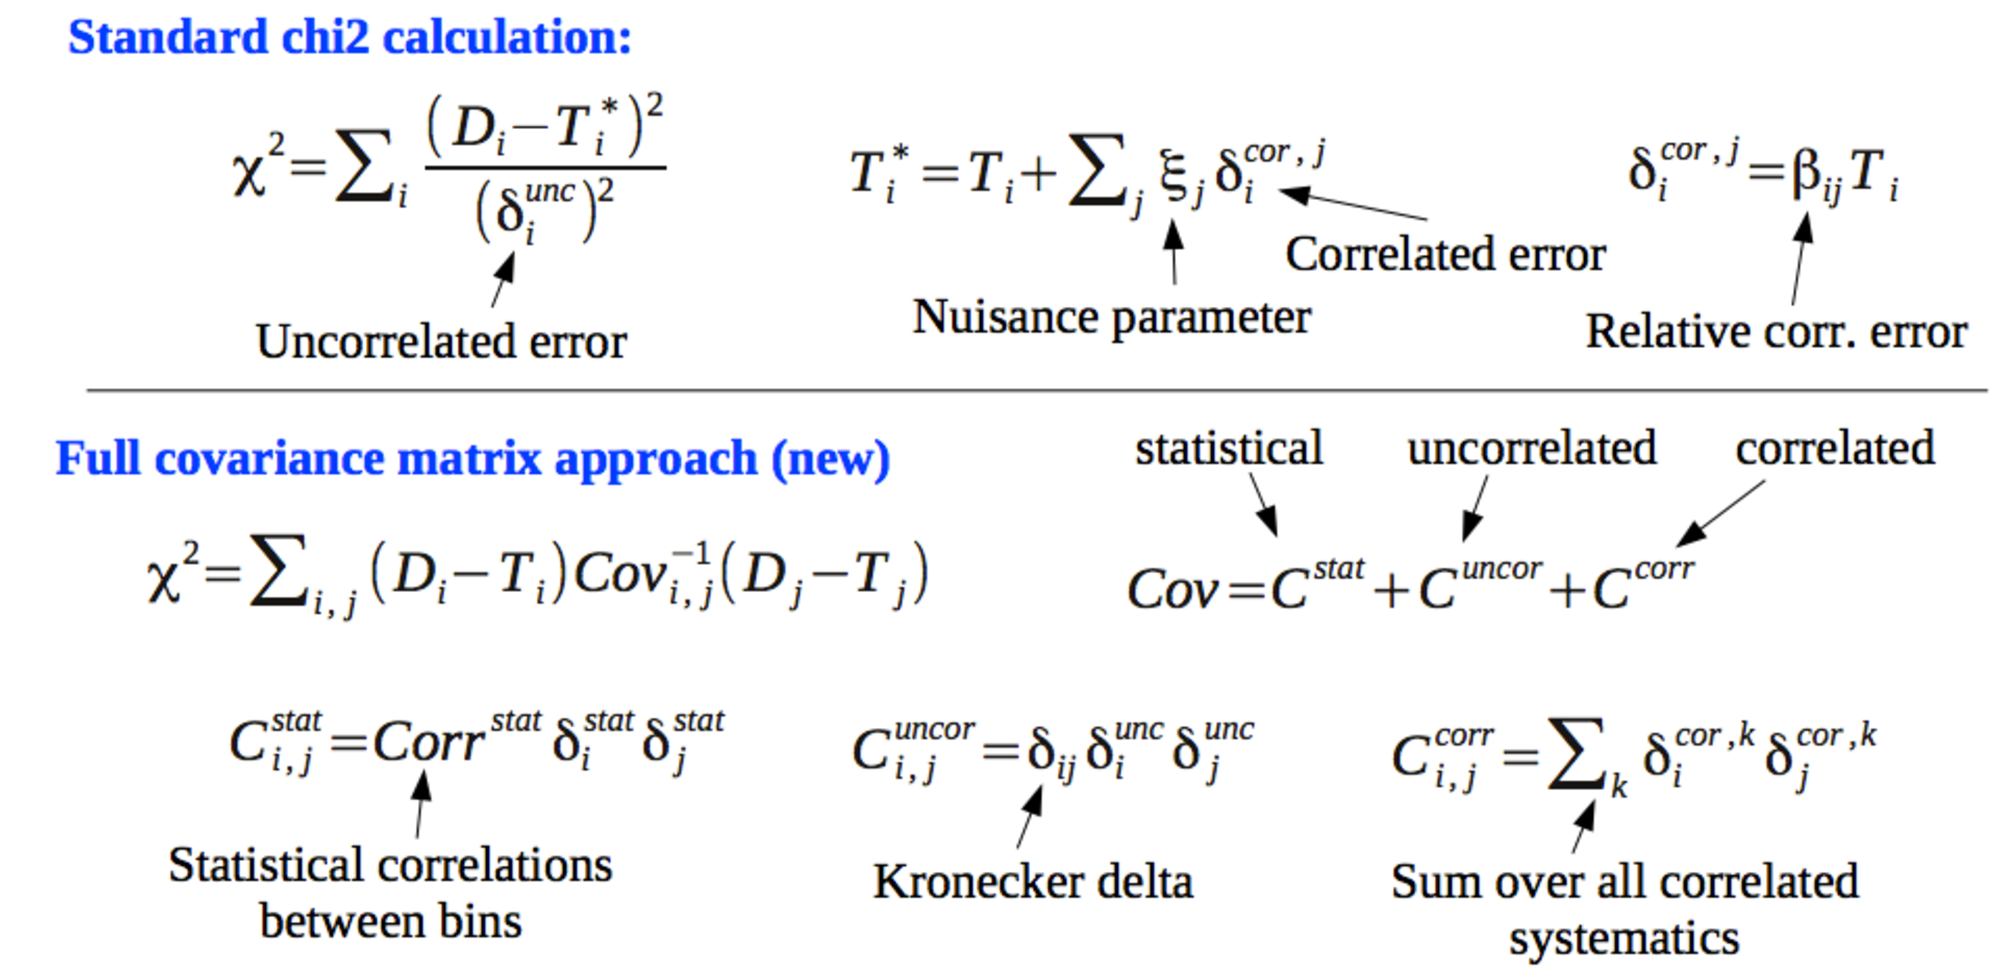
\includegraphics[width=0.75\linewidth]{figures/chi2.pdf}
\end{center}
\label{fig:org}
\end{figure}
 The description starts with most simple cases and it extends to 
 more evolved form that takes into account the
 possible biases arising from low statistics data. 



\subsection{Using Nuisance Parameters}
%%%%

In this subsection the focus is on the $\chi^2$ using nuisance parameters. Different variants are discussed.



%%%%
\subsubsection{Simple and Scaled Form}

For a single data set, the $\chi^2$ function can be defined in a simple form 
\begin{equation}
 \chi^2_{\rm exp}\left(\boldsymbol{m},\boldsymbol{b}\right) = %\\
%~~~=
 \sum_i
 \frac{\left[m^i
- \sum_j \gamma^i_j m^i b_j  - {\mu^i} \right]^2}
{ \textstyle \left(\delta_{i,{\rm stat}}m^i\right)^2 +
\left(\delta_{i,{\rm uncor}}\,  m^i\right)^2}
 + \sum_j b^2_j.
\label{eq:ave}\end{equation}
%
or more evolved as~\cite{H1:2009bp},

%
\begin{equation}
 \chi^2_{\rm exp}\left(\boldsymbol{m},\boldsymbol{b}\right) = %\\
%~~~=
 \sum_i
 \frac{\left[m^i
- \sum_j \gamma^i_j m^i b_j  - {\mu^i} \right]^2}
{ \textstyle \delta^2_{i,{\rm stat}}\mu^i \left(m^i -  \sum_j \gamma^i_j m^i b_j\right)+
\left(\delta_{i,{\rm uncor}}\,  m^i\right)^2}
 + \sum_j b^2_j.
\label{eq:ave}\end{equation}
%
Here ${\mu^i}$ is the  measured central value  at a point $i$ 
with  relative statistical $\delta_{i,stat}$ 
and relative uncorrelated systematic uncertainty $\delta_{i,unc}$.
Further, $\beta_j$ denotes a nuisance parameter for
 a correlated systematic error  source of type $j$ with an uncertainty
 while
$\gamma^i_j$ 
quantifies the sensitivity of the
measurement ${\mu^i}$ at the point $i$ to the systematic source $j$. 
The function $\chi^2_{\rm exp}$ depends on the set of
underlying physical quantities $m^i$ 
(denoted as the vector $\boldsymbol{m}$) and 
 the set of systematic uncertainties $b_j$ ($\boldsymbol{b}$).
This definition of the $\chi^2$ function takes into account that
systematic uncertainties are proportional to the central values 
(multiplicative errors), whereas the statistical errors scale 
with the square roots of the expected number of events. 
Other scaling properties for the statistical and uncorrelated
systematic uncertainties 
are discussed later.



In the case of off-diagonal statistical uncertainties, the $\chi^2$ function
is
\begin{equation} \label{eq:chi2gen}
\chi^2_{\rm exp} (\boldsymbol{m},\boldsymbol{b}) = \sum_{ij} \left ( m^i - \sum_l \Gamma^i_l(m^i)b_l - \mu^i \right)
  C^{-1}_{{\rm stat.}~ij}(m^i,m^j) \left(  m^j - \sum_l \Gamma^j_l(m^j)b_l - \mu^j \right) + 
\sum_l b^2_l \,.
\end{equation}
Here the scaling properties of the correlated systematic uncertainties 
$\Gamma^i_j$ and
of the covariance matrix $C_{{\rm stat.}~ij}$ are expresses as a dependence
on $m_i$ and the dependence of $\Delta_{\rm stat}$ on $b_j$ is ignored.

Eq.~\ref{eq:chi2gen} allows for two methods for fast determination
of the minimum, without need to include the formal nuisance parameters
corresponding to the systematic error sources into the minuit minimisation.
In the first method, the minimisation vs. $b_j$ is used to define covariance
matrix for the systematic uncertainties which is determined as
\begin{equation}
 C_{{\rm syst}~ij}= \sum_l \Gamma^i_l \Gamma^j_l \,.
\end{equation}
The total covariance matrix is given by the sum of the statistical and
systamtic covariance matrices
\begin{equation} 
C_{{\rm tot}~ij} = C_{{\rm stat}~ij} + C_{{\rm syst}~ij}\,,
\end{equation}
and the $\chi^2$ function takes a form
\begin{equation}
  \chi^2( \boldsymbol{m}) = \sum_{ij} ( m^i - \mu^i) C^{-1}_{{\rm tot}~ij} 
( m^j - \mu^j)\,.
\end{equation}

The second methods is used to determine optimal shifts of the nuisance
parameters at each iteration. The shifts are given by minimising 
Eq.~\ref{eq:chi2gen} vs. $b_l$ which leads to a system of  linear equations 
\begin{equation}
 \sum_k \sum_{ij} C^{-1}_{{\rm stat}~ij} \Gamma^i_l \Gamma^j_k \cdot b_k = \sum_{ij} C^{-1}_{{\rm stat}~ij} \Gamma^i_l (m^j - \mu^j)\,,
\end{equation}
where $1\le l \le N_{\rm syst}$, the total number of correlated systematic uncertainties.

Finally the nuisance parameters $\boldsymbol{b}$ can be excluded from the $\chi^2$ minimisation.  
In this case, which is referred to as an Offset method, the minimum is determined for their values set to zero
while uncertainties on the parameters $\boldsymbol{p}$ are determined by shifting each nuisance parameter $b_l$
by $\pm 1$. The total covariance matrix for parameters $p^i$ is determined as 
\begin{equation}
  C^{\rm offset}_{ {\rm par}~ ij} = \sum_{l=1}^{N_{syst}} \Delta p^i_l \Delta p^j_l \,,
\end{equation}
where $ \Delta p^i_l = 0.5 ( p^i( b_l = +1 ) - p^i(b_l = -1))$ and the quality of the fit is estimated by 
fixing $\boldsymbol{p}$ to the value at the minimum and minimising with respect to $\boldsymbol{b}$

Finally, all three approaches can be combined together. For example, only some of the systematic uncertainties
can be treated using the matrix method while others can be treated using the hessian method. In this case, the
covariance matrix  $C_{\rm syst}$ is build using the corresponding sub-set of systematic sources and $C_{\rm stat}$ 
is replaced by $C_{\rm stat}+C_{\rm syst}$ in Eq.~\ref{eq:chi2gen}. Similarly, some of the systematic uncertainties
can be treated using offset method and then $C^{\rm total}_{ {\rm par}} = C^{\rm hessian}_{\rm par} + C^{\rm offset}_{\rm par}$
where offset and hessian covariance matrices are calculated using corresponding systematic error sources.

\subsection{Bias corrections}

The correlated and uncorrelated systematic uncertainties can be treated as additive,  $\Gamma^i_l(m^i) = \gamma^i_l \mu^i$
or multiplicative, $\Gamma^i_l(m^i) = \gamma^i_l m^i$. The LogNormal treatment in which 
$ \mu^i + \sum_l \Gamma^i_j b_l$ is replaced by $ \mu^i \prod_l \exp( \gamma^i_j b_l) $ is forseen for the
next release of the {\tt HERAFitter}. 

The statistical uncertainties can be treated as additive, $\Delta^i(m^i) = \delta^i \mu^i$  and as Poisson,
$\Delta^i(m^i) = \delta^i \sqrt{\mu^i m^i}$. More complex scaling from Eq.~\ref{eq:ave}, 
which depends on shifts of $b_j$, is implemented using an iterative approach: for the first iteration $b_l =0$ 
 is used to determine values of $b_l$ which are then applied in the second iteration. Statistical covariance
matrix is scaled in a similar manner. In this case the correlation matrix is assumed to be fixed, the diagonal
ellements are updated using the prescription describe above and the covariance matrix is rescaled accordingly.

The modifications of the covariance matrix at each iteration of the minuit minimisation may lead to systematic
biases. There are two approaches to avoid these biases. In the first approach the covariance matrix is calculated
using the expected values at the first iteration of the minimisation and kept fixed to these values for further
iterations. This method requires several repetitions of the minimisation, to ensure that values close to optimal
are obtained already at the first iteration. The second method modifies the $\chi^2$ function by adding a term
corresponding to non-constant value of the covariance matrix:
\begin{equation}
 \chi^2_{\rm log} = 2 \log \frac{\Delta^i(m^i)}{\Delta^i(\mu^i)} 
\end{equation}  

\subsection{HERAFitter implementation}
The form of the $\chi^2$ function and the scaling properties of the 
uncertainties are controlled globally by the {\sc CHI2SettingsName} and
{\sc  Chi2Settings} variables and individually using {\sc ``:''} modifiers.
The global scaling properties of the uncertainties are described in 
Table~\ref{tab:ErrScale}. The global form of the $\chi^2$ function
is defined by the {\sc CorChi2Type} parameter, see   
Table~\ref{tab:Chi2Type}.

The default behaviour can be changed for each correlated systematic source by ``:'' modifiers.
They are described in Table~\ref{tab:SystModifier}. The modifiers should appear at the end 
of the systematic source name, e.g. {\sc 'H3:M'}. Several modifiers can be used, e.g. {\sc 'H3:M:C'}.

The names of systematic error sources are read first from the {\sc ListOfSources} variable of the 
{\sc \&Systematics} namelist, located in the {\sc steering.txt} file. Next the names are read from the
data files following the sequence given by the {\sc InputFileNames} list. The properties of each systematic
error source are defined by its first occurence. That means that if, for example, {\sc 'H3:M:C'} is defined
in the {\sc ListOfSources} variable, the source {\sc 'H3'} is treated as multiplicative and using covariance
matrix approach regarless definitions in the data files. If, however, {\sc ListOfSources} defines a souce
without any modifiers, e.g. {\sc 'H3'}, the default treatment, following the {\sc Chi2Settings} variable is
enforced for this source.
Thus the {\sc ListOfSources } variable is a convinient way to modify behaviour of the correlated systemat
sources.

The shifts of the systematic sources are reported in the {\sc Results.txt} file. The uncertainty on the shift
is however estimated only approximately, neglecting the correlation with the theory parameters. An accurate determination
of the uncertainty can be achived by using the toy MC method (see Section~\ref{sec:ToyMC}) or by using {\sc ':E'} 
modifier. In the later case the systematic source is treated using the {\tt Minuit} minimisation. Note, however,
that this approach can slow the minimisation convergence considerably.
\begin{table}
\begin{center}
\begin{tabular}{ccccc} 
\hline
 Option  & {\sc StatScale} & {\sc UncorSysScale} & {\sc CorSysScale} & Scaling rule \\
\hline
  {\sc Poisson}   &  $+$  &  $+$  &  $-$  & $\sqrt{ m^i \mu^i}$ \\
  {\sc Linear}    & $-$   &  $+$  &  $+$  & $m^i$               \\
  {\sc NoRescale} & $+$   &  $+$  &  $+$  & $\mu^i$   \\
  {\sc LogNorm}   &  \multicolumn{4}{c}{Reserved, not implemented} \\
\hline
\end{tabular}
\end{center}
\caption{\label{tab:ErrScale}Global scaling rules for statistical, 
uncorrelated and correlated systematic uncertainties. The scaling
rule is given with respect to corresponding relative uncertainty.
E.g. for the {\sc Poisson} statistical uncertainty the absolute statistical
uncertainty is $\Delta_i = \delta_{i, {\rm stat}}\sqrt{m^i\mu^i}$   }
\end{table}

\begin{table}
\begin{center}
\begin{tabular}{cl}
\hline
    {\sc CorChi2Type} value &  Description \\
\hline
  {\sc Hessian}             & Use nuisance parameters.\\
  {\sc Matrix }             & Use covariance matrix. \\
  {\sc Offset }             & Use offset method\\
\hline
\end{tabular}
\end{center}
\caption{\label{tab:Chi2Type}Possible values of the {\sc CorChi2Type} parameter which defines treatment of the correlated systematic uncertainties.}
\end{table}
 
\begin{table}
\begin{center}
\begin{tabular}{cl}
\hline
  Modifier &  Description \\
\hline
   \multicolumn{2}{c}{Scaling properties}\\
  {\sc :M}  &  Multiplicative scaling, $ m^i$ \\
  {\sc :A}  &  Additive scaling, $ \mu^i$ \\
  {\sc :P}  &  Poisson scaling, $ \sqrt{m^i\mu^i}$ \\
   \multicolumn{2}{c}{$\chi^2$ treatment}\\
  {\sc :N}  &  Nuisance parameter treatment \\
  {\sc :C}  &  Covariance matrix treatment \\
  {\sc :O}  &  Offset method treatment \\
  {\sc :E}  &  Nuisance parameter, included in {\sc Minuit} (``External'')\\
\hline
\end{tabular}
\end{center}
\caption{\label{tab:SystModifier}Modifiers for correlated systematic
uncertainty sources.}
\end{table}
% available as described in appendix~\ref{sec:herafitter}.
%%%%
%\subsubsection{Generalised Scaled Form}

%%%%%%%%%%%
%\subsection{Using Covariance Matrix}
%%%%%%%%%%%%%%%%%%%%%%%%%%%%%


\subsection{Treatment of the Experimental Uncertainties}
\label{sec:error}
%%%%%%%%%%%
%\subsection{Hessian Method}

%%%%%%%%%%%
%\subsection{Offset Method}

\newcommand{\rs}{s}
\newcommand{\ce}{b}
\DeclareRobustCommand\Vstat{\ensuremath{V^{\mathrm{(unc)}}}}
\DeclareRobustCommand\Vsys{\ensuremath{V^{\mathrm{(cor)}}}}
\DeclareRobustCommand\mb[1]{\ensuremath{\mbox{\mathversion{bold}{$#1$}}}}
\DeclareRobustCommand\mbs[1]{\ensuremath{\mbox{\mathversion{bold}{\scriptsize $#1$}}}}

\subsection {Correlated errors and \texorpdfstring{$\chi^2$}{chi2}}
\label{sec:cor-chi2}

% \cite{Chekanov:2002pv,Pascaud:1995qs}
% A typical formula for $\chi^2$ depending on the correlated systematic errors' fluctuations reads
Results of a measurement can be modelled as
(see eg.~\cite{Stump:2001gu,Botje:2001fx})
\begin{equation}
m_n = t_n(a) + r_n \sigma_n + \sum_{\mu=1}^K \rs_\mu \ce_{n\mu}
\;,\quad n=1,\dots,N
\end{equation}
where\\
$m_n$ is the value measured for the $n$-th data point,\\
$t_n(\mb a)$ is true (theoretical) value depending on parameters $\mb a = (a_1,\dots, a_M)$,\\
$\sigma_n$ is the uncorrelated error,\\
$\ce_{n\mu}$ are the errors from the $\mu$-th correlated error source,\\
$r_n$ and $\rs_\mu$ are random variables fluctuating around 0 with unit dispersion.

First, we assume that all $r_n$ are uncorrelated with $\rs_\mu$,
mutually independent and normally distributed,
%  with the statistical errors.
\begin{equation}
\rho(r) = \frac{e^{-r^2/2}}{\sqrt{2\pi}}
\,.
\end{equation}

In the following we will use scaled variables
\begin{subequations}
\begin{eqnarray}
x_i &\equiv& \frac{m_i-t_i}{\sigma_i}
\,,
\\
\beta_{i\mu} &\equiv& \frac{\ce_{i\mu}}{\sigma_i}
\,.
\end{eqnarray}
\end{subequations}

Keeping $\mb \rs$ fixed we get the probability density of measurements,
\begin{equation}
dp(\mb{m}| \mb s) =
 (2\pi)^{-N/2}\, e^{-\chi_1^2(\mbs\rs)/2}\, d^Nx
\,,
\end{equation}
where
\begin{equation}
\label{eq:chi1}
\chi_1^2(\mb\rs) = \sum_{n=1}^N
\left( x_n - \sum_\mu \beta_{n\mu} \rs_\mu \right)^2
\equiv (\mb{x - \beta s})^2
\,,
\end{equation}

Further, taking into account the probability distribution of the correlated error sources,
$p(\mb s)\, d^Ks$, we have
\begin{equation}
p(\mb{m},\mb s) = p(\mb s)\, p(\mb{m} | \mb s)
\,.
\end{equation}
Assuming again the uncorrelated normal distribution,
\begin{equation}
p(\mb s) = \prod_{\mu=1}^K \frac{e^{-s_\mu^2/2}}{\sqrt{2\pi}}
\,,
\end{equation}
we get
\begin{equation}
\label{eq:p_ms}
dp(\mb{m},\mb s) =
  (2\pi)^{-(N+K)/2}\, e^{-\chi_{\mathrm c}^2(\mbs\rs)/2}
  \,d^Nx\, d^Ks
\,,
\end{equation}
with
\begin{equation}
\label{eq:chi_c}
\chi_{\mathrm c}^2(\mb\rs) = 
% (\mb{x - \beta s})^{\mathrm{T}} (\mb{x - \beta s}) + \mb s^{\mathrm{T}} \mb s
(\mb{x - \beta s})^2 + \mb s^2
\,.
\end{equation}

This quadratic form in $\mb s$ allows for analytical integration of Eq~\ref{eq:p_ms}
resulting in

\begin{equation}
p(\mb{m}) \propto e^{-\chi^2/2}
\,,
\end{equation}
where
\begin{equation}
\label{eq:chi_int}
\chi^2 = \mb x^{\mathrm{T}} \mb{A\,x}
\end{equation}
% with constant $\mb A$ determined by $\mb\beta$ and $\mb\sigma$
with $\mb A$ depending on $\mb\beta$ only
(see eg. \cite{Stump:2001gu} Appendix B).

% If we assume that $\rs_\mu$ are random variables with normal distribution, we have
% \begin{equation}
% \tilde\chi^2(\rs) = \sum_{\mu=1}^K \rs_\mu^2
% \end{equation}
% and we can integrate them out analytically.
This is e.g. the CTEQ approach described in \cite{Stump:2001gu}.
It is worth noting that the solution Eq.~\ref{eq:chi_int} for $\chi^2$
can be obtained by minimizing $\chi_{\mathrm c}^2(\mb\rs)$ of Eq.~\ref{eq:chi_c} wrt. $\mb\rs$.

% -----------------------------------
\subsection{The Offset method}

In the Offset method presented here we assume that $\mb\rs$ is fixed, 
and we find the best theoretical model by minimizing
$\chi_1^2$ wrt. to $\mb a$. 
Hence the fitted parameters become functions
of $\mb\rs$. %, $\mb a = \mb a(\mb\rs)$. 
We do not impose any particular statistical properties on $\mb\rs$ 
and we take $\mb a(\mb\rs=0)$ as the ultimate fit result for the theory parameters. 
The dependence on $\mb\rs$ is, however, used to determine
the full error matrix of $\mb a$ (cf. \cite{Pascaud:1995qs}).

The full covariance matrix $V$ reads
\begin{equation}
\label{eq:Cv-full}
V = \Vstat + \Vsys
\end{equation}
% with $\Vsys$ coming from the $\rs$ fluctuations.
For each $\mb\rs$ we find the parameters $\mb a(\mb \rs)$ by minimising $\chi_1^2(\mb \rs)$, which results in
% $a = a(\rs)$ and 
$\Vstat(\mb \rs) = M^{-1}(\mb \rs)$ where
\begin{equation}
M_{jk}(\mb \rs)
= \left.
{\frac12} \frac{\partial^2\chi_1(\mb \rs)^2}{\partial a_j \partial a_k}\right\vert_{\mb a = \mb a(\mb \rs)}
\,.
\end{equation}
The dependence of $M$ on $\mb \rs$ is considered to be a higher order correction
and we take $\Vstat = M^{-1}(0)$.
% Nb. $\Vstat$ is the covariance matrix returned by Minuit for the fit with $\mb \rs =0$.

Within linear approximation to the error propagation
\begin{equation}
\label{eq:Vsysp}
\Vsys_{jk} = \sum_\mu \frac{da_j}{d\rs_\mu} \frac{da_k}{d\rs_\mu}
% \,.
\end{equation} 
and we calculate the derivatives as
\begin{equation}
\frac{da_j}{d\rs_\mu} \approx
\frac{a_j(\rs_\mu=\epsilon) - a_j(\rs_\mu=-\epsilon)}{2\epsilon}
% \,,
\end{equation}
with $\mb a(\rs_\mu=\epsilon)$ resulting from
fits to the data shifted by $\epsilon\ce_{n\mu}$.

In the code we use $\epsilon=1$, i.e. one standard deviation of
the correlated error source which, in the ideal statistical limit, corresponds to 
$\Delta\chi_1^2 = 1$.
On the other hand, within the leading approximation, the value of $\epsilon$ is irrelevant.
% in accordance to the standard Minuit normalization of $\Vstat$.

If another error definition, $\Delta\chi_1^2 = \lambda$, 
is adopted\footnote{E.g. Jon Pumplin uses $\lambda=5$, cf. \texttt{minuit/iterate.F}} then
the full covariance matrix, $V$, must be scaled by $\lambda$. 


%%%%%%%%%%%
\subsection{Monte Carlo Method}
\label{sec:ToyMC}

The PDF uncertainties can be estimated using a Monte Carlo technique \cite{mcmethod}.
The method consists in preparing replicas of data sets by allowing the central values of the cross sections to 
fluctuate within their systematic and statistical uncertainties taking into account all point-to-point correlations.
The preparation of the data is repeated for a large $N$ ($>100$ times) and for each of these replicas a NLO QCD fit is performed to 
extract the PDF set. The PDF central values and uncertainties are estimated using the means values and RMS 
over the replicas. 



%%%%%%%%%%%
\subsection{Regularisation methods}

Regularisation methods are aiming to study the parametrisation assumptions on PDFs. When more flexible parametrisation styles is used the shape of the PDFs must be constrained and various methods could be used.
HERAFitter framework provides the means to study and compare various methods.

%The methods described in this section work for large data sets. 
\subsubsection{Data Driven Regularisation}
This method was first applied by NNPDF group which uses redundant parametrisation and introduces a stopping criteria based on data.
The data driven regularisation method splits data randomly into ``fit'' and ``control''  samples. The ``fit'' sample is used to determine PDF parameters. The $\chi^2$ of this sample is observed to semi-monotonically decrease. The ``control'' sample is used to protect againts over-fitting and for this sample the $\chi^2$ will first decrease and then will start to increase due to fluctuation of the sample.


\subsubsection{External Regularisation based on penalty term in $\chi^2$}

Another method to constrain the PDF shape is to simply apply a penalty term
to the $\chi^2$ function. 
One method is so called ``length penalty'' which selects PDF solutions with smoother shape in $W\approx Q\sqrt{\frac{1-x}{x}}$:
\begin{equation}
L=\int_{W_{min}}^{W_{max}} \sqrt{1+\left(\frac{dxf(W)}{dW}\right)^2}dW
\end{equation}
This method can be applied when using Chebyshev polynomials to parametrise PDFs.
For more details, the reader is invited to look up the \cite{Chebyshev} reference.

For the case when using flexible parametrisation style, 
a $\chi^2$ penalty term is applied to account for a deviation 
from a simple PDF parametrisation form such as:
\begin{equation}
\chi^2_{reg}= T\sum_f\left(\left(\frac{D_f}{\Delta_D}\right)^2+ \left(\frac{E_f}{\Delta_E}\right)^2\right),
\end{equation}

with $\Delta D=\Delta E = 100$, such that for large $D$ and $E$ the ratio will approach $1$. The $T$ is the regularisation parameters, such that for $T=0$ there is no penalty term and for large $T$ there is strong penalty.


\section{Bayesian Reweighting Technique}
\label{sec:reweighting}
Bayesian reweighting of PDF sets is a way to include new data into an existing PDF set without actual carrying out a full-blown fitting procedure. It has been first suggested by Giele and Keller~\cite{Giele:1998gw} and first pursued in practice by the NNPDF Collaboration~\cite{Ball:2011gg,Ball:2010gb}. Watt and Thorne~\cite{Watt:2012tq} proposed a scheme of how to implement the Bayesian reweighting technique also for PDF predictions based on central values with errors determined using the Hessian Eigenvector Method. 

The \fitter package allows to update any PDF that is either available as probability distribution (i.e. a lhapdf .LHgrid file in NNPDF format) or as PDF eigenvector set (i.e. any PDF set in lhapdf .LHgrid file format with errors determined using the Hessian Eigenvector Method). This enables the user to assess the impact of new data not only for the {\tt HERAPDF} using the full-blown fit procedure but also for the other standard global PDF sets and allows to compare how the data impacts different PDFs.

The Bayesian Reweighting technique essentially uses PDF probability distributions as input, applies weights to these distributions based on how well the new data is described and outputs an updated PDF probability distribution. In the following paragraphs, firstly the construction of these PDF probability distributions is described, then the calculation of the weights to update the PDF probability distribution is introduced and lastly, the configuration of the module within the \fitter framework is explained.

\subsection{PDF probability distributions}

PDF probability distributions are constructed as finite ensembles of $N_{\mathrm{rep}}$ parton distribution functions $\mathrm{PDF}_k$, $\mathcal{E} = \{PDF_k, k = 1, . . . ,N_{\mathrm{rep}}\}$. Observables $\mathcal{O}(\mathrm{PDF})$ are conventionally calculated from the average of the predictions obtained from the ensemble:

\begin{equation}
 \langle\mathcal{O}(\mathrm{PDF})\rangle = \frac{1}{N_{\mathrm{rep}}} \sum_{k=1}^{N_{\mathrm{rep}}} \mathcal{O}(\mathrm{PDF}_k)
\label{eq:meanReplicas}
\end{equation}
 
Their uncertainties are calculated as the standard deviation, defined as:

\begin{equation}
\sigma_{\mathcal{O}(\mathrm{PDF})} = \sqrt{  \frac{1}{N_{\mathrm{rep}} - 1 }  \sum_{k=1}^{N_{\mathrm{rep}}} 
( \mathcal{O}(\mathrm{PDF}_k) - \langle \mathcal{O}(\mathrm{PDF})  \rangle   )^2     
     }
\end{equation}

While the standard PDF sets from the NNPDF collaboration are already available as ensembles of parton distribution functions, the PDF predictions of other PDF fitting groups need to be converted to PDF probability distributions. This is possible provided that the PDF sets have associated uncertainties that can be used to create replicas of the central PDF set with random variations that lie within the uncertainties. 

In the case of uncertainties provided by standard Hessian eigenvectors error sets, this can be easily achieved by creating the $k$-th random replica by introducing to the central PDF set, $\mathrm{PDF}_0$, random fluctuations. 

If the PDF eigenvectors are asymmetric, that is they come in pairs of negative and positive PDF error sets, corresponding to negative and positive deviations from the central value, these random fluctuations are created by drawing a random number $R_{jk}$ and adding, depending on the sign of the random number, the difference of the positive or respectively negative PDF of the $j$-th PDF eigenvector pair from the central value, scaled by the absolute value of the random number:

\begin{equation}
 \mathrm{PDF}_k = \mathrm{PDF}_0  + \sum_{j=0}^{n} \left[ \mathrm{PDF}^{\pm}_j - \mathrm{PDF}_0 \right] |R_{jk}|
\end{equation}
 
Here, $k$ denotes the number of the random replica and runs from $k=1, ... , N_\mathrm{rep}$; $j$ denotes the eigenvector pair and runs from $j=1, ..., n$, where $n$ is the number of eigenvectors, e.g. $n=20$ for MSTW08. 

In case, the Hessian eigenvectors are symmetrised and only one error set is given per eigenvector, the above prescription simplifies to:
   
\begin{equation}
 \mathrm{PDF}_k = \mathrm{PDF}_0  + \sum_{j=0}^{n} \left[ \mathrm{PDF}_j - \mathrm{PDF}_0 \right] R_{jk}
\end{equation}

\subsection{Bayesian Reweighting of PDF sets}

Once PDF probability distributions are available as inputs, they can be updated to incorporate the new data. This is achieved by applying weights to the PDF probability distributions such that the prediction for observable $\langle\mathcal{O}(\mathrm{PDF})\rangle$ from equation \ref{eq:meanReplicas} changes to:

\begin{equation}
 \langle\mathcal{O}^{\mathrm{new}}(\mathrm{PDF})\rangle = \frac{1}{N_{\mathrm{rep}}} \sum_{k=1}^{N_{\mathrm{rep}}} w_k \mathcal{O}(\mathrm{PDF}_k)
\end{equation}

The weights $w_k$ calculated are here according to:

\begin{equation}
 w_k = \frac{(\chi^2_k)^{\frac{1}{2} (N_{\mathrm{data}}-1) } \exp^{-\frac{1}{2}\chi^2_k}}{ \frac{1}{N_{\mathrm{rep}}} \sum^{N_{\mathrm{rep}}}_{k=1}(\chi^2_k)^{\frac{1}{2}(N_{\mathrm{data}}-1)} \exp^{-\frac{1}{2}\chi^2_k}  },
\end{equation}

where $N_{\mathrm{data}}$ is the number of new data points, $k$ denotes the specific replica for which the weights is calculated and $\chi^2_k$ is between a given data point $y_i$ and its theoretical prediction obtained with the $k$-th PDF replica:

\begin{equation}
 \chi^2 (y,\mathrm{PDF}_k) = \sum_{i,j=0}^{N_{\mathrm{data}}} (y_i - y_i(\mathrm{PDF}_k)) \sigma^{-1}_{ij} (y_j-y_j(\mathrm{PDF}_k))  
\end{equation}

The weighted PDF probability distribution can be turned into a new ensemble of PDF replicas, based on which predictions for any observable can be calculated. This new, reweighted PDF probability distribution commonly is chosen to be based upon a smaller number of PDF sets compared to the input PDF probability distribution, in order throw away those replicas that are incompetible with the data and to create a more light-weight PDF set. 


\subsection{Usage of the PDF reweighting in the \fitter framework}
 
The \fitter allows to perform PDF reweighting for NNPDF-style PDF probability distributions as well as for PDF sets with Hessian PDF error Eigenvector sets. 

This requires the {\tt NNPDF reweight} and the {\tt LHAPDF} modules to be installed, see sections \ref{sec:install_nnpdfrweight} and \ref{sec:install_lhapdf}. In the \fitter steering files, the PDF reweighting needs to be switched on and the relevant parameters have to be set: 

\begin{itemize}
 \item \textbf{FLAGRW}: En/disable reweighting
 \item \textbf{RWPDFSET}: Name of the PDF set to be reweighted
 \item \textbf{RWDATA}: Arbitrary name for the data to be updated, used to create the names of the output PDF set and the directory
 \item \textbf{RWMETHOD}: Do the reweighting based on chi2 (method 1, where you read in \fitter data files and theory predictions and calculate the chi2 based on them) or on data (method 2, where you have to provide an input text file with theoretical predictions {--} the input format of these will be explained below)
 \item \textbf{DORWONLY}: Disable the usual PDF fit, such that only the reweighting is done 
 \item \textbf{RWREPLICAS}: Number of input replicas used for the PDF probability distributions (not applicable for NNPDF sets, since they come with a fixed number of replicas)
 \item \textbf{RWOUTREPLICAS}: Number of replicas in the output PDF set.
\end{itemize}

The setup of the module is such, that it is parsing the \fitter steering file and from the specified settings creates a special reweighting steering file in the directory {\tt input\_steering} with the pattern {\tt <RWPDFSET>\_<RWDATA>\_<RWMETHOD: chi2 or data>.in}. 

In the output directory, a subdirectory is created for the output of the reweighting procedure. Its name pattern is: {\tt output/<RWPDFSET>\_<RWDATA>\_<RWMETHOD: chi2 or data>/} and it will contain the following files:

\begin{itemize}
 \item {\tt <RWPDFSET>\_<RWDATA>\_<RWMETHOD: chi2 or data>\_nRep<RWOUTREPLICAS>.LHgrid}: The output PDF probability distribution in form of an .LHgrid file, which allows easy usage.
 \item {\tt whist-rw.eps}: Plot with the distributions of weights calculated for each replica. The meaning of this variable is further described in~\cite{Ball:2011gg,Ball:2010gb}.
 \item {\tt palpha-rw.eps}: Plot with the probability for each replica to describe the data. The meaning of this variable is further described in~\cite{Ball:2011gg,Ball:2010gb}.
 \item {\tt <RWPDFSET>\_<RWREPLICAS>InputReplicas.LHgrid}: This is the PDF probability function that has been produced from the eigenvector PDF sets produced by the Hessian method (not applicable for NNPDF sets).
\end{itemize}

 
%%%%%%%%%%%%%%%%%%%%%%%%%%%%%%


%%%%%%%%%%%%%%%%%%%%%%%%%%%%%%

\newpage
\section{Program Manual}
\label{sec:progman}
This section begins with a presentation of the installation instructions for various scenarios supported by the \fitter\ platform.
There then follows a basic user manual which is intended to guide the user in his/her analysis.

\subsection{Program Installation Instructions} 

\label{sec:install}
%%%%%%%%%%%

To install {\fitter} together with the most commonly used modules it is suggested to use the default installation script:

{\scriptsize
{\tt https://wiki-zeuthen.desy.de/xFitter/xFitter/DownloadPage?action=AttachFile\&do=view\&target=install-xfitter}
}

If you want to install the package manually, use the following instruciton.

\subsubsection{Core Installation and Modules}
The Installation Instructions are dependent on which modules are activated via the configuration option. To see complete list of options and possible
modules, run
\begin{verbatim}
./configure --help
\end{verbatim}
\subsubsection{Pre-requirements}

The \fitter\ program has been tested on various platforms:\\
 SL6 (64 bit),  Ubuntu 14.04, Mac OS.  The following programs and system libraries are required:
\begin{itemize}
 \item {\tt gfortran}, {\tt gcc} and {\tt g++}  comiliers.   
 \item {\tt lapack}, {\tt blas} libraries
\end{itemize}

The following package is required in order to build the \fitter\ package:
\begin{itemize}
\item QCDNUM~\cite{qcdnum} versions starting from {\tt qcdnum-17-01-11} should be used. These can be found at \\
  {\tt http://www.nikhef.nl/$\sim$h24/qcdnum/QcdnumDownload.html}
\end{itemize}

%%%%%%%%%%%
\subsubsection{Default Minimal Installation}
\begin{itemize}
\item
 Makesure that \qcdnum installation directory is added to the executabel
 path and that {\tt LD\_LIBRARY\_PATH} points to the \qcdnum libraries.
 To verify that, type
\begin{verbatim}
 qcdnum-config  --libdir
\end{verbatim}
and check that the printed directory is indeed included in the {\tt LD\_LIBRARY\_PATH} list.

\item Run:
\begin{verbatim}
    ./configure
    make 
    make install
\end{verbatim}
If your system does not have {\tt root} analysis package installed, you can use the {\fitter} core functionality, however certain packages such as {\tt xfitter-draw} 
can not be built. The support of these programs is included by default and thus 
{\tt root} package is required when you run {\tt configure} script without 
additional options. You may disable root by configuring using 
{\tt configure --disable-root} option.


After these commands are finished, the executable {\tt bin/xfitter} 
file should be installed
\item  Run a check:
\begin{verbatim}
    bin/xfitter 
\end{verbatim}
\end{itemize}
%%%%%%%%%%%
\subsubsection{Installation with external packages
( \applgrid, \apfel, \mela, \lhapdf )}
\begin{itemize}
\item Make sure that \qcdnum bin directory and libraries are included
in the paths as described in the previous section
\item Make sure that {\tt \$PATH} and {\tt \$LD\_LIBRARY\_PATH} 
variables point to the external package(s) enviroment.
\item Run:
\begin{verbatim}
   # For applgrid only:
    ./configure --enable-applgrid 
   # For mela only:  
   # ./configure --enable-mela 
   # For apfel only:
   # ./configure --enable-apfel
   # For lhapdf only 
   # ./configure --enable-lhapdf
   # For all packages:
   #  ./configure --enable-applgrid  --enable-mela  --enable-apfel  --enable-lhapdf

    make 
    make install
\end{verbatim}
After these commands are finished, the executable {\tt bin/xfitter} 
file should be installed
\item  Run a check:
\begin{verbatim}
    bin/xfitter 
\end{verbatim}
\end{itemize}
%%%%%%%%%%%


%%%%%%%%%%%
\subsubsection{Installation with {\tt HATHOR}}
 Note that support of {\tt HATHOR} is suspended in {\fitter}. Please use
 this option with extra caution.
 \begin{itemize}
  \item Download Hathor from 
\begin{verbatim}
http://www-zeuthen.desy.de/~moch/hathor/
\end{verbatim}
     and install it according to the instructions given there
     (requires \verb'LHAPDF' library)

  \item Define a variable HATHOR\_ROOT  such that HATHOR\_ROOT  points to the
     directory of your Hathor installation

  \item Install the \fitter\ as described above but configuring it
     with the option "--enable-hathor" before building it
 \end{itemize}


%%%%%%%%%%%
%\subsection{Installation with {\tt CASCADE}}
\subsubsection{Installation for TMD (uPDF) in high-energy factorisation (using  {\tt CASCADE})}

\begin{itemize}

\item Installation with TMD requires Cascade and Pythia generators, 
they can be downloaded from\\
{\tt http://cascade.hepforge.org/ } and 
{\tt https://pythia6.hepforge.org/ } respectively. \\
        \\
After installation of the generator packages, the {\tt CASCADE\_ROOT}  and {\tt PYTHIA\_ROOT} 
environment variables have be specified and point to the corresponding libraries. 
In the DESY afs environment the pre-installed versions of Cascade and Pythia can be used:  
%
{\footnotesize\begin{verbatim}
export CASCADE\_ROOT=/afs/desy.de/group/alliance/mcg/public/MCGenerators/cascade/2.2.04/\$SYSNAME 
export PYTHIA\_ROOT=/afs/desy.de/group/alliance/mcg/public/MCGenerators/pythia6/425/\$SYSNAME}
\end{verbatim} }
\normalsize
where {\tt SYSNAME } = i586\_rhel50 or similar.

\item Run:
\begin{verbatim}
    ./configure --enable-updf --enable-lhapdf
    make 
    make install
\end{verbatim}


\item use steering and \minuit input files from "input\_steering": 

   \begin{verbatim} 
   cp input-steering/steering.txt.kt-factorisation steering.txt 
   cp input-steering/minuit.in.txt.kt-factorisation minuit.in.txt 
   cp input-steering/steer-ep-CASCADE steer-ep 
   cp input-steering/steer_gluon-evolv steer_gluon-evolv
    \end{verbatim}

\item  edit steering.txt: 
   \begin{verbatim}
   \&CCFMFiles: give name for output grid file for uPDF   
   \&\fitter\ 
   TheoryType = 'uPDF3' ! 'DGLAP'  -- collinear evolution
                ! 'uPDF'   -- un-integrated PDFs:
                !  uPDF1 fit with kernel ccfm-grid.dat file
                !  uPDF2 fit evolved uPDF, fit just normalisatio
                !  uPDF3 fit using precalculated grid of sigma_hat
                !  uPDF4 fit calculating kernel on fly, grid of sigma_hat
  \end{verbatim}
  The recommended option is \verb+uPDF4+, which evolves the evolution kernel for gluons and valence quarks
  (evolution parameters are set in \verb+steer_gluon-evolv+). After evolution of the kernel, $\hat {\sigma}$ is
  calculated in a grid in $x$ at the  $Q^2$ values used in the data sets selected. The ${\hat \sigma}$ values are   
  stored for transverse and longitudinal cross sections for light quarks ($n_f \leq 3$), charm and beauty quarks.
\item run the program: bin/xfitter 
   
\item plotting $F_2$ fit results: \\
xfitter-draw  can be used to draw $F_2$ results. \\
The uPDFs need to be plotted with an external package (currently not available).
\end{itemize}


\subsection{User Manual}
\label{sec:man}
%%%%%%%%%%%
In this section a user manual is presented. The section starts with a general overview of the code
organisation and it follows with a more detailed explanation for the most frequently used functions.

%%%%%%%%%%%%%%%%%%%%%%%%%%%%%%%%%%%%%%%%
\subsubsection{Code Organisation}
A general diagram of  available modules is illustrated in figure~\ref{fig:org}.
The flow is depicted such that it follows the structure of the \fitter\ .
\begin{figure}
\begin{center}
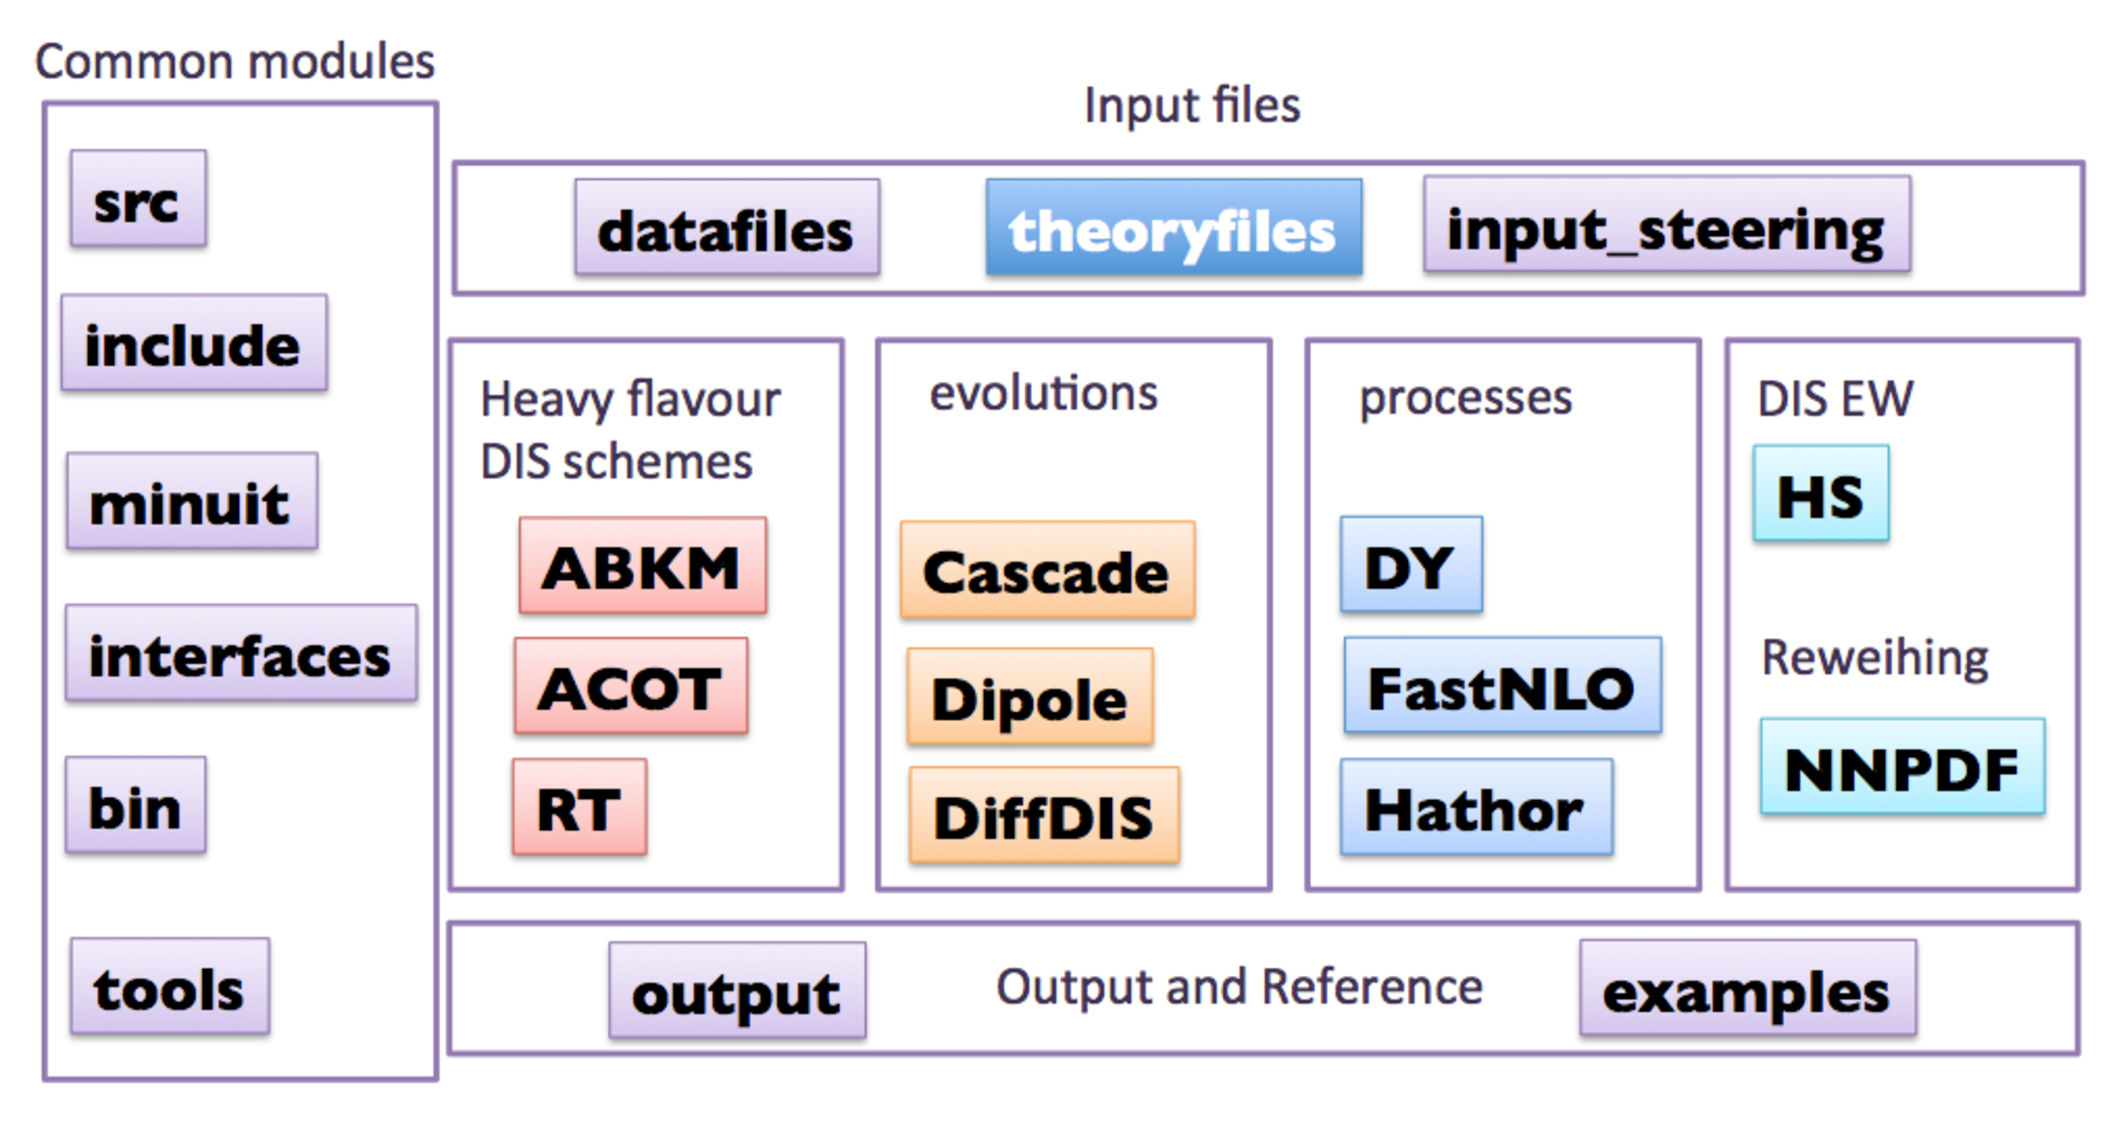
\includegraphics[width=0.75\linewidth]{figures/organisation.pdf}
\end{center}
\caption{Schematic structure of the \fitter\ program organisation in different modules.}
\label{fig:org}
\end{figure}

In addition, an inventory list with short description of existing subroutines is  
presented in Table~\ref{tab:list}. 
Here we choose to enlist only the routines from the common target module to guide 
the user of available functionalities.

\begin{center}
\begin{table}
\begin{tabular}{lp{4cm}p{10cm}}
\hline
\hline
\small\bf{steerings} & $\bullet$ steering.txt:& free PDF parameters to be varied by MINUIT \\
 & $\bullet$ minui.in.txt:& main steering card \\
 & $\bullet$ ewparam.txt:& settings of electroweak parameters, as well as masses \\
\toprule
\bf{src} & $\bullet$ main.f:& main program \\
& $\bullet$ read\_steer.f: &access steer parameters from steering card \\
& $\bullet$ read\_data.f: & reading the datatables and storing data information \\
& $\bullet$ init\_theory.f: & initialising theory modules \\
& $\bullet$ dataset\_tools.f:&  allocating bin indices \\
& $\bullet$ error\_logging.f: &  error logging information\\
& $\bullet$ minuit\_ini.f: & initialise minuit module \\
& $\bullet$ fcn.f: & passes to minuit the $\chi^2$ to be minimised \\
& $\bullet$ pdf\_param.f:  &  parametrisation of the PDFs at starting scale\\
& $\bullet$ sumrules.f: & PDF constraints at starting scale, such as QCD sum rules. \\
& $\bullet$ evolution.f: & evolution of PDFs \\
& $\bullet$ theory\_dispatcher.f: & distribution of theory prediction calculations for a given dataset  \\
& $\bullet$ dis\_sigma.f & calulates the DIS cross sections \\
& $\bullet$ GetChisquare.f & calculates the $\chi^2$  \\
& $\bullet$ GetCovChisquare.f & calculates the $\chi^2$ using covariance matrix \\
& $\bullet$ GetPointScaledErrors.f & calculates the rescaled statistical, uncorrelated and constant errors \\
& $\bullet$ prep\_corr.f & prepare systematic correlation matrix \\
& $\bullet$ systematics.f & build the matrix for systematic uncertainties and invert it \\
& $\bullet$ error\_bands\_pumplin.f  & Hessian error calculations  \\
& $\bullet$ mc\_errors.f & MC method for creating replicas of data through smearing. \\\cmidrule{2-3}
& $\bullet$ GetDiffDisXsection.f  & calulates the diffractive DIS cross sections \\
& $\bullet$ FixModelParams.f  & used for diffractive DIS cross sections \\\cmidrule{2-3}
& $\bullet$ lhapdf\_dum.f   & \tiny (used only with ENABLE\_LHPDF)\\
& $\bullet$ reweighting.f & main subroutine for PDF rewighting \tiny (used only with ENABLE\_NNPDF) \\
& $\bullet$ nnpdfreweighting.f & main subroutine for NNPDF rewighting \tiny (used only with ENABLE\_NNPDF) \\\cmidrule{2-3}
& $\bullet$ dy\_cc\_sigma.f  & calulates the DY cross sections \\
& $\bullet$ applgrids\_dum.f    & protective file against miss-use of flags in steering\\
& $\bullet$ fappl\_grid.cxx  &  \tiny (used only with ENABLE\_APPLGRID) \\
& $\bullet$ applgrids.f    &  passing PDFs to APPLGRID \tiny (used only with ENABLE\_APPLGRID) \\
& $\bullet$ pp\_jets\_applgrid.f   & calulates $pp$ jets cross sections  \\
& $\bullet$ ep\_jets\_fastnlo.f  &  calulates $ep$ jets cross sections \\\cmidrule{2-3} 
& $\bullet$ getncxskt.f  & access the NC cross sections grids for uPDFs\\
& $\bullet$ Getgridkt.f & acess the grids for uPDFs \\\cmidrule{2-3}
& $\bullet$  ttbar\_hathor\_dum.f  & protective file against miss-use of flags in steering\\
& $\bullet$  ttbar\_hathor.f  & \tiny ( used only with ENABLE\_HATHOR) \\\cmidrule{2-3}
& $\bullet$ offset\_fns.f & collects results from Offset method and stores them\\
& $\bullet$  g\_offset.cc  & file used for Offest method\\
& $\bullet$  matrix.cc  & inversion of matrix as used for Offset method \\
& $\bullet$  FitPars\_base.cc  & file used for Offest method\\
& $\bullet$  FTNFitPars.cc   & file used for Offest method\\
& $\bullet$  Xstring.cc   & file used for Offest method\\
& $\bullet$  decor.cc   & file used for Offest method\\\cmidrule{2-3}
& $\bullet$ store\_output.f & write the output  \\
& $\bullet$ store\_h1qcdfunc.f & store structure functions   \\
\bottomrule
\end{tabular}
\caption{A list of main subroutines are listed with a short description of their function.}
\label{tab:list}
\end{table}
\end{center}

%%%%%%%%%%%%%%%%%%%%%%%%%%%%%%%%%%%%%%%%
\subsubsection{Steering files}
 The software behavior is controlled by three files with steering commands.
 These files have predefined names:
    
\begin{itemize}
      \item {\tt steering.txt}  --   controls main "stable" (un-modified during 
                         minimisation) parameters. The file also contains
                         names of data files to be fitted and definitions 
                         of kinematic cuts                              
      \item {\tt minuit.in.txt}
                   --  controls minimisation parameters and minimisation 
                         strategy. Standard Minuit commands can be provided
                         in this file
      \item {\tt ewparam.txt}    --  controls electroweak parameters such
        as W and Z boson masses and CKM matrix parameters.
\end{itemize}


%%%%%%%%%%%%%%%%%%%%%%%%%%%%%%%%%%%%%%%%

\begin{description}
\item \bf{Steering.txt}\rm 

Different options are activated via steering flags in the main steering file.
%and the default steering file is displayed in figure  \ref{fig:steering}.
 
The format of the steering file follows standard "namelist" conventions.
Comments start with exclamation mark (similarly used for data file format).
The following namelist blocks are encountered:
\begin{itemize}
\item  {\tt InFiles}: Namelist to control input data
\item  {\tt InCorr}: Namelist to control statistical correlation files
\item  {\tt Scales} (Optional): Namelist to modify renormalisation/factorisation scale
\item  {\tt HeraFitter}: Main steering cards. 
%Further details can be found in the appendix \ref{sec:herafitter}. 
\item  {\tt ExtraMinimisationParameters}:  Namelist to add extra to minuit parameters.
\item  {\tt Output}: Namelist that outputs steering cards 
\item  {\tt Cuts}: Namelist for process dependent cuts
\item  {\tt MCErrors} (Optional):Namelist for MC errors steering cards
\item  {\tt Cheb} (Optional): Chebyshev study namelist
\item  {\tt Poly} (Optional): pure polynomial parameterisation for valence quarks
\item  {\tt HQScale} (Optional): choose the factorisation scale for HQs
\item  {\tt lhapdf} (Optional):LHAPDF steering card
\item  {\tt reweighting} (Optional): reweighting steering cards
\end{itemize}

These namelist blocks are described in greater details in the User's example \ref{section:example}. 


\begin{description}
\item \it\bf Theory type: \rm\\
 
here is a steering flag which defines the theory type via the chosen evolution.
The following types are supported:
\begin{itemize}
\item \tt{TheoryType = 'DGLAP' }\rm as used for collinear evolution theories. For this type another 
 flag is needed to specify the order of the perturbative series in $\alpha_S$:
\tt{Order}\rm which can be leading order (LO), next-to-leading order (NLO) and when available NNLO.
\item \tt{TheoryType = 'DIPOLE' }\rm as used for the dipole models;
\item \tt{TheoryType = 'uPDF' }\rm as used for the un-integrated PDFs (with 4 variants)
\end{itemize}

\item \it\bf Starting scale: \rm\\
The evolution starting scale is set via flag  \tt{Q02}\rm, commonly set below charm threshold, as imposed by QCDNUM.

\item \it\bf Scheme type: \rm\\
For the DIS process, several schemes are available for heavy quark treatments via  \tt{HF\_SCHEME}\rm flag.
\begin{itemize}
  \item VFNS (Variable Flavour Number Schemes):
    \begin{itemize}
     \item RT-VFNS  schemes                               [from Robert Thorne], \tt{HF\_SCHEME = RT, RT OPT}\rm, as well as the fast variants based on k-factors \tt{RT FAST, RT OPT FAST}
     \item Zero Mass VFNS                                 [qcdnum], \tt{ZM-VFNS}\rm   
     \item  ACOT (ACOT-Full, ACOT-ZM, S-ACOT-Chi) schemes  [from Fred Olness], \tt{HF\_SCHEME = ACOT Full, ACOT Chi, ACOT ZM}\rm, they are all based on k-factors. 
    \end{itemize}
  \item FFNS (Fixed Flavour Number Scheme)
    \begin{itemize}
    \item via QCDNUM, \tt{HF\_SCHEME = FF}\rm 
    \item via ABM (openqcdrad-1.6)   [from Sergey Alekhin], \tt{HF\_SCHEME = FF ABM}\rm
    \end{itemize}
\end{itemize}
IMPORTANT to note if running with FFNS (nf=3): 
\begin{itemize}
  \item only neutral current DIS data should be used in FF scheme due to missing NLO 
    coefficient functions in charged current process, in this cases valence quark parameters  
    need to be fixed in minuit.in.txt file.
  \item In FF ABM implementation the charged current coefficients are available
    therefore valence parameters do not need to be fixed.
  \item $\alpha_s(Q^2)$ in FFNS is 3-flavour and recommended to be set to the value of 0.105 
    such that is not too high at low energies
  \item the scale in FFNS is defined as $\mu^2 = Q^2 + 4m_h^2$ by default, can be 
    changed in HQScale in \tt{steering.txt}\rm (scale variation in ABM not yet implemented)
  \item  the pole mass definition for heavy quarks is set in ABM by default, 
    the running mass definition \cite{Alekhin:runm} can be switched in 
    by setting \tt{HF\_SCHEME = FF ABM RUNM} \rm in \tt{steering.txt} \rm. 
\end{itemize}

\item \it\bf PDF parametrisation style: \rm\\
There are various types of parametric functional form supported by \fitter\ .
They are accessed via the steering flag called \tt{PDFStyle}\rm. Available styles
are summarised as follows:

\begin{tabular}{ll}
 \tt  '10p HERAPDF'   & -- HERAPDF-like with extra assumption Buv = Bdv \\
 \tt   '13p HERAPDF' & -- HERAPDF-like with Buv and Bdv floated independently and two fur-\\
                     &  ther free parameters for the gluon PDF which allow it to be negative at \\
                     &  low scale\\
 \tt   '10p H12000'  & -- H12000-like (D,U,Dbar,Ubar+g) \\
 \tt   'CTEQ'        & -- CTEQ-like parameterisation \\
 \tt   'CHEB'        & -- CHEBYSHEV parameterisation based on glu, sea, uval, dval evolved\\
                     &  pdfs \\
 \tt  'LHAPDFQ0'    & -- use lhapdf library to define pdfs at starting scale and evolve with local \\
                    &  qcdnum parameters \\
 \tt  'LHAPDF'      & -- use lhapdf library to define pdfs at all scales\\
 \tt   ' DDIS'        & -- use Diffractive DIS \\
 \tt  'BiLog'       & -- bi-lognormal parametrisation \\
\end{tabular}


These styles were described in details in section~\ref{sec:pdfparam}.
The LHAPDF style can be used only with proper configuration settings,
 as explained in the section~\ref{sec:install}.
\item \it\bf  Definition of Chisquares:\rm\\
Currently two different formats of defining $\chi^2$ are supported.
The new format is explained in the section \ref{sec:chi2}.
%Currently two different styles are supported for a smoother 
%transition to the new style which is more flexible.
The old format corresponds to {\tt CHI2Style}  --- (string) choice of the $\chi^2$ function:\\
\begin{tabular}{ll}
    {\tt 'H12000'}& -- Pascaud-like, systematic shifts to theory, no scaling of statistical, uncorrelated errors.\\
    {\tt 'HERAPDF'}& -- Pascaud-like + "mixed error scaling"\\
    {\tt 'HERAPDF Sqrt'}&   -- Pascaud-like + "sqrt error scaling"\\
    {\tt 'HERAPDF Linear'}& -- Pascaud-like + "linear error scaling"\\
    {\tt 'Offset'}& -- Offset method activated\\
 \end{tabular}

\item \it\bf (logical) debug flag:\rm
 The debug flag will be turned on for more print outs via \tt LDEBUG. \rm

%%%%%%%%%%%%%%%%%%%%%%%%%%%%%%%%%%%%%%%%
%\subsubsection{Selection of the data}
\item \it\bf Selection of the data:\rm \\
  The namelist \&Cuts, located inside the {\tt steering.txt} file can be used to apply
  simple process dependent cuts. The cuts are limited to bin variables.
  Simple low and high limits are allowed. For example, a cut on $Q^2>3.5$~GeV$^2$ for
  NC ep scattering is specified as

\begin{verbatim}
  ! Rule #1: Q2 cuts
   ProcessName(1)     = 'NC e+-p'
   Variable(1)        = 'Q2'
   CutValueMin(1)     = 3.5 
   CutValueMax(1)     = 1000000.0
\end{verbatim}

Maximum 100 cuts can be used by default.
\end{description}


%%%%%%%%%%%%%%%%%%%%%%%%%%%%%%%%%%%%%%%%

The specific input files are stored in the {\tt $input\_steerings$} directory and 
it contains the following ready to use inputs (with corresponding minuit files):

\begin{itemize}
\item  {\tt steering.txt.ALLdata}: all data files 
\item  {\tt steering.txt.DIFFRACTION}: diffraction specific settings 
\item  {\tt steering.txt.kt-factorisation}: kt factorisation specific settings
\item  {\tt steering.txt.dipole}: dipole model specific settings  
\end{itemize}


%%%%
%\subsubsection{Options for Jets}
%%%%
%\subsubsection{Options for Diffractive fits}
%%%%
%\subsubsection{Options for DY fits}
%%%%%%%%%%%

%%%%%%%%%%%%%%%%%%%%%%%%%%%%%%%%%%%%%%%%
\item \bf {{\tt Minuit} steering cards}\rm


The minuit steering card is described below, a sample file is presented 
in Fig.~\ref{fig:minuit}
\begin{figure}
\begin{center}
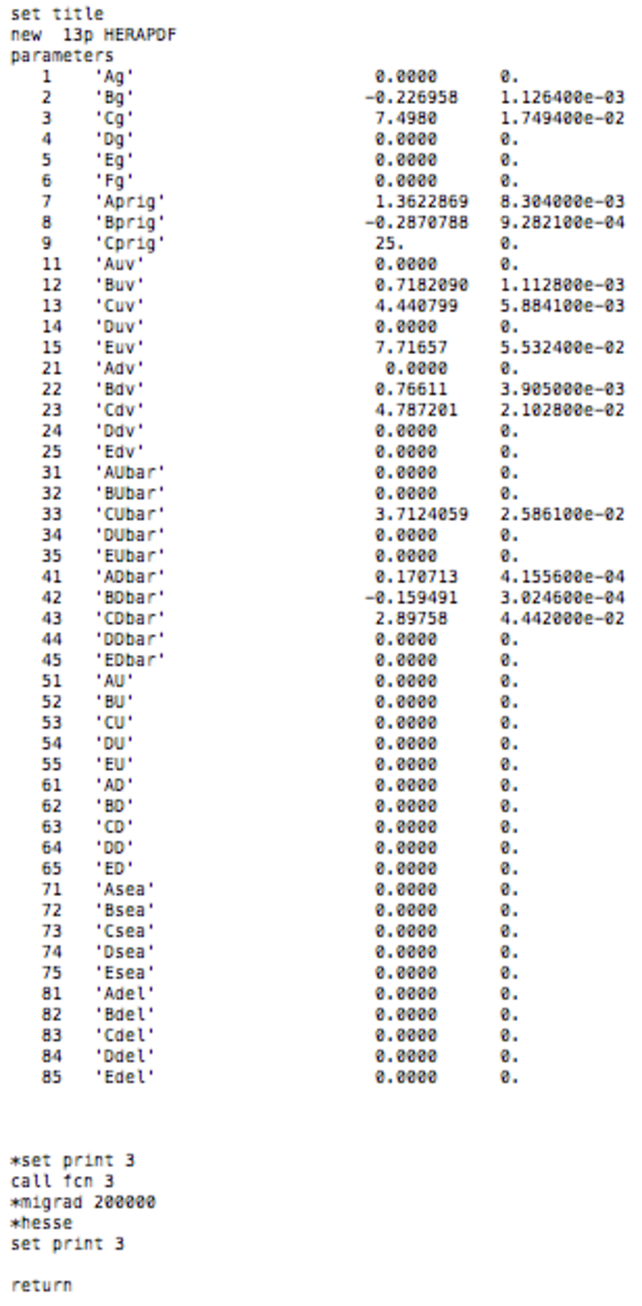
\includegraphics[width=0.45\linewidth]{figures/minuit.pdf}
\end{center}
\caption{An example of a minuit steering card.}
\label{fig:minuit}
\end{figure}

The first three lines set the title and specify the list of MINUIT parameters which are to follow.      
The index of parameters is the first column and it is hardwired to the source code:\\

\begin{tabular}{ll}
1 -10 & gluon parameters \\    
11-20 & uval  parameters \\
21-30 & dval  parameters \\
31-40 & Ubar  parameters \\
41-50 & Dbar  parameters \\
51-60 & U     parameters \\
61-70 & D     parameters \\
71-80 & Sea   parameters \\
81-90 &Delta parameters \\
91-100 & other parameters: alphas (95), fs=Dbar/str (96), fc=Ubar/ch (97)\\
\end{tabular}

The second column represents just user defined names,
the third column is  the input starting value for the parameter.
The forth column sets the step size (usually chosen the same order as the error).
If the step size is zero this parameter is FIXED.
The fifth column sets the lower bound of the fit parameter, 
The sixth column sets the upper bound of the fit parameter
if these columns are not filled then there are no bounds.

Only parameters that have non-zero stepsize are varied 
in the fit (free parameters). Another way to fix the parameters is
simply by typing at the end of the list of parameters ``FIX parameter number''.  
(make sure there is one line free before the minuit list).
Examples of commands taken by minuit are:\\

\begin{tabular}{ll}
call fcn 3  &   fit is not performed, only 1 iteration, useful for testing\\
            &    Minuit parameters ARE NOT minimized. \\
migrad       & fit is performed (default number of calls 2000).\\
migrad 20000 & fit is performed up to 20000 calls, then terminates.\\
hesse        & Hessian estimate of the \tt{MINUIT}\rm parameters \\
& (more reliable than \tt{MINUIT}\rm)\\
\end{tabular}


The output of the fit is stored in the output/ directory as \tt{minuit.out.txt}\rm.
Statements in minuit.out.txt which are useful for interpreting the results of the fit:
\begin{itemize}
\item \tt{FCN=575.16}\rm  \; this is total chisquare
\item \tt{FROM MIGRAD   STATUS=CONVERGED}\rm \; this is desirable for a fit that converged
\item \tt{FROM HESSE     STATUS=OK}\rm       \; this is desirable for a fit that converged 
\item \tt{ERROR MATRIX ACCURATE}   \rm       \; errors estimated with HESSE method
\end{itemize}

{\bf HERAFitter parameters for diffractive fits} \\
%%-----------------------------------------------------------
\label{sec:HFitterPar}

% minuit.in.txt
% ExtraMinimisationParameters

\begin{tabular}{l|l|l}
Parameter & HERAFitter name & input file\\
% \hline
$\Cini {\mathrm G}1$ & Ag & minuit.in.txt \\
$\Cini {\mathrm G}2$ & Bg & minuit.in.txt \\
$\Cini {\mathrm G}3$ & Cg & minuit.in.txt \\
$\Cini {\mathrm S}1$ & Auv & minuit.in.txt \\
$\Cini {\mathrm S}2$ & Buv & minuit.in.txt \\
$\Cini {\mathrm S}3$ & Cuv & minuit.in.txt \\
$\alpha_\Pom(0)$ & Pomeron\_a0 & steering.txt \\
$A_\Reg$ & Reggeon\_factor & steering.txt \\
$\alpha_\Reg(0)$ & Reggeon\_a0 & steering.txt \\
\end{tabular}
\vspace{0.7cm}

{\bf HERAFitter parameters for dipole fits} \\
The default  initial parameters for the fit without valence quarks are : 
\begin{table}[h]
\tiny
\begin{center}
\begin{tabular}{|c||c||c||c|c||c|c|c||c|c|} 
\hline 
$\sigma_0$ & $A_g$ & $\lambda_g$ & $C_g$ & $cBGK$& $eBGK$\\
\hline
37.490 & 3.3446 & 0.0298 & 2.6302 & 4.0 & 15.362 \\
\hline
\end{tabular}
\end{center}
\end{table}
\\
For the BGK dipole model fits with valence quarks the initial parameters and the obtained $\chi^2$ are:

\begin{table}[ht]
\begin{center}
\begin{tabular}{|c||c||c||c|c||c|c|c||c|c|c||c|}
\hline
No&
$Q^2$&&
$\sigma_0$ & $A_g$ & $\lambda_g$ & $C_g$ & $C_{BGK}$& $\mu_{0}^2$& $Np$&
$\chi^2/Np$\\
\hline
1 &
$Q^2 \ge 3.5$ &  LO & 66.6 & 4.0 & -0.039 & 18.6& 4.0 & 5.3  & 196 &  0.930 \\
\hline
2 &
$Q^2 \ge 3.5$ & NLO & 79.4 & 3.2 &-0.021 & 13.7 & 4.0 & 6.7 & 196 & 0.927 \\
\hline
\end{tabular}
\end{center}
\end{table}
\end{description}


%%%%%%%%%%%%%%%%%%%%%%%%%%%%%%%%%%%%%%%%
\subsubsection{Data file format}
\label{sec:dataformat}
   Experimental data are provided by the standard {\tt ASCII} text files. The files
   contain a "header" which describes the data format and the "data" in terms
   of a  table. Each line of the data table corresponds to a
   data point, the meaning of the columns is specified in the file header.

   For example, a header for HERA-I combined H1-ZEUS data for e+p neutral 
   current scattering cross section is given in the file

\begin{verbatim}
       datafiles/H1ZEUS_NC_e-p_HERA1.0.dat
\end{verbatim}

   The format of the file follows standard "namelist" conventions. Comments 
   start with an exclamation mark.  Pre-defined variables are:
\begin{itemize}
     \item{\tt Name}        --- (string) provides the name of the data set
    \item{\tt  Reaction}    --- (string) reaction type of the data set. Reaction type is used 
                      to trigger the corresponding theory calculation. The following 
                      reaction types  are currently supported by the HERAFitter:
                      \begin{itemize}
                        \item {\tt 'NC e+-p'}  -- double differential NC ep scattering
                                      (ZM-VFNS and RT-VFNS schemes) 
                        \item {\tt 'CC e+-p'}  -- double differential CC ep scattering
                                      (ZM-VFNS scheme)
                        \item {\tt 'CC pp'}    -- single differential $d \sigma_{W^{\pm}}/d eta_{\ell^{\pm}}$
                                      production and W asymmetry at $pp$ and $p\bar{p}$ 
                                      colliders (LO+kfactors and APPLGRID interface)
                        \item {\tt 'NC pp'}    -- single differential $d \sigma_Z / d y_Z$ at $pp$ and
                                      $p\bar{p}$ colliders
                                      ({\tt LO} with k-factors and {\tt APPLGRID} interface)

                        \item 'pp jets APPLGRID' -- $pp\to$ inclusive jet production, using
                                     {\tt APPLGRID}

                        \item 'FastNLO jets' -- jet cross sections using {\tt FastNLO} interface.
                                     All $ep$, $pp$ and $p\bar{p}$ colliders are supported.

                        \item 'FastNLO ep jets normalised' -- jet cross sections in the $ep$ collisions 
                                     using {\tt FastNLO} interface and normalised to the inclusive DIS cross sections.

                      \end{itemize}                       
      \item {\tt NData}       --- (integer) specifies number of data points in the file. 
                     This corresponds to the number of table rows which 
                     follow after the header.
      \item {\tt NColumn}     --- (integer) number of columns in the data table.
      \item {\tt ColumnType}  --- (array of strings)
                      Defines layout of the data table. The following column types
                      are pre-defined: 'Bin', 'Sigma', 'Error' and 'Dummy'
                      The keywords are case sensitive. 'Bin' correspond to an
                      abstract bin definition, 'Sigma' corresponds to the data
                      measurement, 'Error' - to various type of uncertainties and
                      'Dummy' indicates that the column should be ignored.
      \item {\tt ColumnName}  --- (array of strings)
                      Defines names of the columns. The meaning of the name depends
                      on the ColumnType. For ColumnType 'Bin', ColumnName gives a
                      name of the abstract bin. The abstract bins can contain
                      any variable names, but some of them must be present for 
                      correct cross section calculation. For example, 'x', 'Q2' and
                      'y' are required for DIS NC cross-section calculation.
 
                      For ColumnType 'Sigma', ColumnName provides a label for 
                      the observable, which can be any string.
 
                      For ColumnType 'Error', the following names have special meaning:
                      \begin{itemize}
                       \item 'stat'  -- specifies column with statistical uncertainties, request Poisson re-scaling;
                       \item 'stat const'  -- specifies column with statistical uncertainties, request no re-scaling of the errors;
                       \item 'uncor' -- specifies column with uncorrelated uncertainties. Any name containing keyword ``uncor'' is treated as an uncorrelated
  error source, e.g. ``h1 uncor'';  
                       \item 'uncor const' -- specifies column with uncorrelated uncertainties, request no re-scaling of the errors;  
                       \item 'total' -- specifies column with total uncertainties. 
                                  Total uncertainties are not used in the fit,
                                  however there is an additional check is performed
                                  if 'total' column is specified: sum in quadrature
                                  of statistical, uncorrelated and correlated 
                                  systematic uncertainties is compared to the total
                                  and a warning is issued if they differ significantly.
                       \item'ignore' - specifies column to be ignored (for special studies).
                       \item Other names specifies columns of correlated systematic 
                      uncertainty. For a given data file, each column of the correlated
                      uncertainty must have unique name. To specify correlation across
                      data files, same name must be used for different files.  
                      \end{itemize}
      \item {\tt SystScales}  --- (array of float)
                      For special studies, systematic uncertainties can be scaled
                      The numbering of uncertainties starts from the first column
                      with the ColumnType 'Error'. For example, setting 
\begin{verbatim}
                  SystScale(1) = 2.  
\end{verbatim}
                      in {\tt datafiles/H1ZEUS\_NC\_e-p\_HERA1.0.dat} would scale systematic 
                      uncertainty by factor of two.                       
      \item {\tt Percent}     --- (array of bool) For each uncertainty specify if it is given in 
                      absolute ("false") or in percent ("true").  The numbering of 
                      uncertainties starts from the first column with the 
                      {\tt ColumnType} 'Error' (see example above).
      \item {\tt NInfo}       --- (integer) Calculation of the cross-section predictions may 
                      require  additional information about the data set. The number of 
                      information strings is given by NInfo
      \item {\tt CInfo}       --- (array of strings) Names of the information strings. 
                      Several of them are predefined for different cross-section 
                      calculations.
      \item {\tt DataInfo}    --- (array of float) Values, corresponding to {\tt CInfo} names.
      \item {\tt IndexDataset} -- (integer) Internal \fitter\ index of the data set. Provide unique
                      numbers to get extra info for $\chi^2/dof$ for each data set.      
      \item {\tt TheoryInfoFile} --- (string) Optional additional theory file with extra 
                     information for cross-section calculation. This could be k-factors,
                     {\tt APPLGRID} file or {\tt FastNLO} table.  
      \item {\tt TheoryType} --- (string) Theory file type can be set to
		     'kfactor', 'applgrid', 'fastnlo' or 'expression'. See further for more
		     details.
      \item {\tt TermName} --- (string) names of terms used in the theory expression.
      \item {\tt TermSource} --- (string) pathes from where the term numerical values should be taken.
      \item {\tt TheorExpr} --- (string) theory epression in simple algebraic form.
      \item {\tt NKFactor}   --- (integer) For kfactor files, number of columns in
                     {\tt TheoryInfoFile}.
      \item {\tt KFactorNames} --- (array of strings) For kfactor files, names of columns in 
                     {\tt TheoryInfoFile}.
\end{itemize}

Depending on the chosen process specific requirements for the header might be present. 
Dataset-wise options are provided by a {\tt CInfo} / {\tt DataInfo} variable set. In case the information
varies between data points (e.g. bin borders, hadronisation corrections etc.) it is
provided in the data file and recognised by the program using reserved column names.
In the following all these requirements are listed and briefly explained.

The theory type {\it expression} allows a flexibility in theory definition, making
it possible to set a simple formula in {\tt TheorExpr} string variable.  The
expression terms must be preliminary defined in {\tt TermName} -- a string value, 
starting with alphabetical character, {\tt TermType} -- recognized string values are 'kfactor',                                                                                        
'applgrid' or 'virtgrid', and {\tt TermSource} -- the files from where the
predictions are taken. {\tt TermType} defines which type of the expression term
is used:
\begin{description}
\item[kfactor] is a term wich denotes an array of \(K\)-factors corresponding
  to the data bins. The {\tt TermSource} for this term must point to a file with the 
  \(K\)-factor table, containing three columns: bin lower and higher edges, and the
  \(K\)-factor value. The comments starting with ``\#'' are ignored.
\item[applgrid] term tells the parser to initialize the APPLgrid grid for the
  cross section evaluation. The grid options are defined with additional options
  in {\tt DataInfo} and {\tt CInfo}.
\item[virtgrid] can be used if the fit is performed on the multidimensional 
  measurement results. The {\tt TermSource} in this case is a text file with a virtual
  grid definition. Consider for example the data are
  a triple differential measurement of a cross section in \(X\), \(Y\) and \(Z\)
  observables. Internally the theory prediction for such measurement is
  represented as a linear array -- a sequence of applgrids for \(Z\), each
  corresponding to the hyperbin in \(X\) and \(Y\). The virtual grid file in 
  this case is a table, where each row denotes the hyperbin with its edges,
  APPLgrid file location and number of bins in it:
  \begin{align*}
  X_0^{\mrlow} &\quad X_0^{\mrhigh} \quad Y_0^{\mrlow} \quad Y_0^{\mrhigh} \quad {\mrpa}\_0\_0{\mrdrt} &\quad M(0;0) \\
  X_0^{\mrlow} &\quad X_0^{\mrhigh} \quad Y_1^{\mrlow} \quad Y_1^{\mrhigh} \quad {\mrpa}\_0\_1{\mrdrt} &\quad M(0;1) \\
  \ldots \\
  X_0^{\mrlow} &\quad X_0^{\mrhigh} \quad Y_{N_Y}^{\mrlow} \quad Y_{N_Y}^{\mrhigh} \quad {\mrpa}\_0\_N_Y{\mrdrt} &\quad M(0;N_Y) \\
  X_1^{\mrlow} &\quad X_1^{\mrhigh} \quad Y_{0}^{\mrlow} \quad Y_{0}^{\mrhigh} \quad {\mrpa}\_1\_0{\mrdrt} &\quad M(1;0) \\
  X_1^{\mrlow} &\quad X_1^{\mrhigh} \quad Y_{1}^{\mrlow} \quad Y_{1}^{\mrhigh} \quad {\mrpa}\_1\_1{\mrdrt} &\quad M(1;1) \\
  \ldots \\
  X_{N_X}^{\mrlow} &\quad X_{N_X}^{\mrhigh} \quad Y_{0}^{\mrlow} \quad Y_{0}^{\mrhigh} \quad {\mrpa}\_N_X\_0{\mrdrt} &\quad M(N_X;0) \\
  \ldots \\
  X_{N_X}^{\mrlow} &\quad X_{N_X}^{\mrhigh} \quad Y_{N_Y}^{\mrlow} \quad Y_{N_Y}^{\mrhigh} \quad {\mrpa}\_N_X\_N_Y{\mrdrt} &\quad M(N_X;N_Y) \\
  \end{align*}
  where \(N_X,\,N_Y\) are the numbers of hyperbins in \(X,\,Y\) repectively and
  \(M\) is the number of bins in the corresponding applgrid. The order of hyprebin
  listing must be same as for the data table and the slowest changing hyperbin 
  must go first. In case the fitted data is a double-differential cross section, only 
  one hyperbin needs to be listed, i.e.:
  \begin{align*}
  X_0^{\mrlow} &\quad X_0^{\mrhigh} \quad {\mrpa}\_0{\mrdrt} &\quad M(0) \\
  X_1^{\mrlow} &\quad X_1^{\mrhigh} \quad {\mrpa}\_1{\mrdrt} &\quad M(1) \\
  \ldots \\
  X_{N_X}^{\mrlow} &\quad X_{N_X}^{\mrhigh} \quad {\mrpa}\_N_X{\mrdrt} &\quad M(N_X) \\
  \end{align*}
  The comments starting with ``\#'' are ignored.
\end{description}
The expression recognises simple arithmetic operations
(+,-,/,*) and 'sum()' function which returns prediction summed over bins.
Example:
\begin{verbatim}
 TheoryType     = 'expression'
 TermName = 'A1', 'K'
 TermType = 'applgrid','kfactor'
 TermSource = 'path/to/grid.root' ,
              'path/to/kfactor.txt'
 TheorExpr= 'K*A1'
\end{verbatim}
The expression also recognises numerical terms, e.g.  'K*A+0.1', which do not
require preliminary definition. Due to technical limitations, no spaces are
allowed in {\tt TheorExpr} value. 

By default the numeric result of the expression is divided by the (hyper)bin
width. In order to obtain initial values or use 'sum()' operation (integral of
the differential distribution e.g. for normalization purposes) one should add
`\_norm' suffix to the the TermType of 'applgrid' or 'virtgrid'. For example: 
\begin{verbatim}
 TheoryType     = 'expression'
 TermName = 'V', 'A'
 TermType = 'virtgrid','applgrid_norm'
 TermSource = 'path/to/virtgrid.txt' ,
              'path/to/applgrid.root'
 TheorExpr= 'V/sum(A)'
\end{verbatim}

An example of virtgrid.txt file:
\begin{verbatim}
# y1     y2     applgrid                                        n_grid_bins
0.0     0.3     theoryfiles/atlas/Jets2010-vg/R04/eta1.root        17
0.3     0.8     theoryfiles/atlas/Jets2010-vg/R04/eta2.root        17
0.8     1.2     theoryfiles/atlas/Jets2010-vg/R04/eta3.root        17
1.2     2.1     theoryfiles/atlas/Jets2010-vg/R04/eta4.root        16
2.1     2.8     theoryfiles/atlas/Jets2010-vg/R04/eta5.root        13
2.8     3.6     theoryfiles/atlas/Jets2010-vg/R04/eta6.root        10
3.6     4.4     theoryfiles/atlas/Jets2010-vg/R04/eta7.root         7
\end{verbatim}


%%%%%%%%%%%%%%%%%%%%%%%%%%%%%%%%%%%%%%%%
\begin{description}
\item \bf{Data format requirements for DIS}\rm

In this subsection we describe specific requirements for files using 'NC e+-p' and 'CC e+-p'
reaction types. Examples of such input files are:

{\tt datafiles/H1ZEUS\_NC\_e-p\_HERA1.0.dat}

{\tt datafiles/H1ZEUS\_CC\_e-p\_HERA1.0.dat}.

The properly formatted DIS input files will have the following fields available
in the {\tt CInfo} variable list: 

\begin{itemize} 
    \item  {\tt 'sqrt(S)'} --- the ep collision centre-of-mass energy in GeV. In particular, for 
    HERA based results the the corresponding {\tt DataInfo} value should be $300.$ for measurements
    based on data collected prior to $1997$ (inclusive) and $318.$ for data collected after 1997.
    
    \item {\tt 'reduced'} --- a field indicating whether calculated cross section should be reduced (1.) or not (0.)
    (reference to proper equation somewhere in this manual).
    
    \item {\tt 'e charge'} --- electric charge of the colliding lepton beam. Supported {\tt DataInfo} values
    are '1.' for electron and '-1.' for positron.

    \item {\tt 'e polarity'} --- polarity of the lepton beam. The corresponding {\tt DataInfo} value 
    should be between $-1.0$ and $1.0$ (is this true?) with abs($1.0$) indicating fully polarised
    beam and $0.0$ fully unpolarised one. 

    In case of non-vanishing polarity the following additional fields are required:

    \item {\tt 'pol err unc'} --- explain

    \item {\tt 'pol err corLpol'} --- explain
 
    \item {\tt 'pol err corTpol'} --- explain

\end{itemize}

The inclusive DIS cross sections are calculated on an x-Q$^2$-y grid. Correspondingly,
the following columns need to present in the correctly formatted input file: 
{\tt 'x'}, {\tt 'Q2'} and {\tt 'y'}.


%%%%%%%%%%%%%%%%%%%%%%%%%%%%%%%%%%%%%%%%

\item \bf{Data format requirements for FastNLO} \rm

In this subsection we describe data format specific for the FastNLO implementation
accessed by choosing 'FastNLO jets' and 'FastNLO ep jets normalised' reaction types.
Examples of properly formatted files are:

   {\tt datafiles/HERA/ZEUS\_InclJets\_HighQ2\_98-00.dat}

   {\tt datafiles/HERA/H1\_NormInclJets\_HighQ2\_99-07.dat}.

{\tt TheoryType = 'FastNLO'} indicates usage of the FastNLO. The variable {\tt ThoryInfoFile} 
should contain the proper path to the FastNLO table in version 2.0 or higher.
\fitter\ supports both flexible and inflexible scales.
Older FastNLO tables can be still accessed through the APPLGRID interface.

The following fields are required to be present in the {\tt CInfo} list:

\begin{itemize}

    \item {\tt 'PublicationUnits'} --- The desired units in which the cross sections 
    are calculated by the FastNLO code. If the corresponding {\tt DataInfo} field is 
    set to '1.' the cross sections will be given in the same units as used in the
    relevant publication. In the case it is set to '0.', absolute cross section
    units will be used. 

    \item {\tt 'MurDef', 'MufDef'} --- The renormalisation and factorisation scale definitions
    used with variable scale FastNLO tables. If the chosen FastNLO table does not support 
    variable scales, these fields will be ignored and the scale embedded within the table will 
    be used instead. The values of the corresponding {\tt DataInfo} fields set 
    the renormalisation scale $\mu_r$ and factorisation scale $\mu_f$ following the FastNLO standard:
    \begin{align*} 
       \text{value} :&\quad \text{definition} \\
       0 :&\quad   \mu_{r/f}^2 = \mu_1^2 \\
       1 :&\quad   \mu_{r/f}^2 = \mu_2^2 \\
       2 :&\quad   \mu_{r/f}^2 = ( \mu_1^2 + \mu_2^2 )\\
       3 :&\quad   \mu_{r/f}^2 = ( \mu_1^2 + \mu_2^2 ) / 2 \\
       4 :&\quad   \mu_{r/f}^2 = ( \mu_1^2 + \mu_2^2 ) / 4 \\
       5 :&\quad   \mu_{r/f}^2 = (( \mu_1 + \mu_2 ) / 2 )^2\\
       6 :&\quad   \mu_{r/f}^2 = (( \mu_1 + \mu_2 ))^2\\
       7 :&\quad   \mu_{r/f}^2 = \text{max}( \mu_1^2, \mu_2^2)\\
       8 :&\quad   \mu_{r/f}^2 = \text{min}( \mu_1^2, \mu_2^2) \\
       9 :&\quad   \mu_{r/f}^2 = (\mu_1 * exp(0.3 * \mu_2)) ^2
   \end{align*}

   where $\mu_1$ and $\mu_2$ are specific scales chosen during production of the table. In particular
   for jet production at HERA traditionally 
   \begin{equation*}
          \mu_1^2 = Q^2 \quad \quad \quad \mu_2^2 = p_T^2
    \end{equation*}  

   \item {\tt sqrt(S)} --- Should be defined only for 'FastNLO ep jets normalised' reaction type. 
         The ep collision centre-of-mass energy in GeV. In particular, for 
         HERA based results the the corresponding {\tt DataInfo} value should be $300.$ for measurements
         based on data collected prior to $1997$ (inclusive) and $318.$ for data collected after 1997.

   \item {\tt 'lumi(e-)/lumi(tot)'} --- Should be defined only for 'FastNLO ep jets normalised'
         reaction type. The normalisation depends on the ratio of the luminosities of the positron and electron data 
         used for the cross section measurement. This ratio should  be
         given in a format (lumi($e^-$) / (lumi($e^-$) + lumi($e^+$)) and ashould take values between [0., 1.].

   \item {\tt 'UseZMVFNS'} --- Should be defined for 'FastNLO ep jets normalised' reaction type. The calculation
         of the integrated inclusive DIS cross sections could be time consuming.
         This option provides an opportunity to use a "Zero Mass Variable Flavour
         Number Scheme" approximation which is very fast and provides
         enough precision for normalisation purposes. ZMVNS is used if 
         the corresponding {\tt DataInfo} field is set to 1. Otherwise, the same scheme
         is used as defined globally with the variable 'HF\_SCHEME' defined in steering.txt file.
\end{itemize}


In addition there are some specific values within the {\tt ColumnName} field which allow
information specific to each data point to be passed. They are listed below:

\begin{itemize}
     \item{\tt 'Z0Corr'} --- (optional) The correction due to the $Z_0$ boson exchange.
                 If it is given, each point calculated by the FastNLO code will be
                 multiplied by the {\tt Z0Corr} value.

     \item{\tt 'NPCorr'} --- (optional) The non-perturbative correction.
                 If it is given, each point calculated by the FastNLO code will be
                 multiplied by the {\tt NPCorr} value. {\tt Z0Corr} and {\tt NPCorr} can be added 
                 simultaneously, and in this case the calculated cross sections
                 will be multiplied by the product {\tt Z0Corr} * {\tt NPCorr}.

    \item{\tt 'q2min', 'q2max', 'ymin', 'ymax', 'xmin', 'xmax'} --- Should be defined for 
         'FastNLO ep jets normalised' reaction type and are used to define 
         DIS phase space for the normalisation. Since these three ({\tt q2, y, x}) are 
         connected by the relation
         \begin{equation}
              Q^2 = x \cdot y \cdot s
         \end{equation}
         only two are required to be present to unambiguously define the DIS phase space for each data point.
        
\end{itemize}
\end{description}


%%%%%%%%%%%%%%%%%%%%%%%%%%%%%%%%%%%%%%%%
\subsubsection{Understanding the output}
  The results of the minimization are printed to the standard output and written
  to files in the {\tt output/} directory. 

  The quality of the fit can be judged based on the total $\chi^2$ per degrees of freedom.
  It is printed for each iteration as 
\begin{verbatim}
                      Iteration   Chi2   NDF       Chi2/NDF
   FitPDF f,ndf,f/ndf      3      588.64 579        1.02
\end{verbatim}
  The resulting $\chi^2$ is reported at the end of minimisation for each data set and for the correlated 
  systematic uncertainties separately. This information is printed and written
  to the {\tt output/Results.txt} file. The {\tt Results.txt} file contains additional 
  information about shifts of the correlated systematic uncertainties.

  The minimization information from the {\tt minuit} program is stored using the standard {\tt minuit} output format in the {\tt output/minuit.out.txt}
  file. The level of verbosity for this information can be changed by {\tt minuit} commands
  in the {\tt minuit.in.txt} file. 
  It is a good idea to check that minuit does not report any errors
  or warnings at the end of minimisation.
  
  Point by point comparison of the data and predictions after the minimization 
  is provided in the file stored in {\tt output/fittedresults.txt}. The file reports three columns
  corresponding to the three first bins of the input tables, data value, sum in 
  quadrature of statistical and uncorrelated systematic uncertainty, total
  uncertainty and then the predicted value, before and after applying correlated systematic shifts,
  the pull between the  data and theory and 
  the data set index. The pull $p$ is calculated as 
  \begin{equation}
      p = \frac{ \mu - m} {\sigma_{\rm uncor}}
  \end{equation}
  where $\mu$ is the data value, $m$ is the prediction and $\sigma_{\rm uncor}$ is the total
  uncorrelated uncertainty.
  Similar information is stored in the {\tt pulls.first.txt} and {\tt pulls.last.txt} files
  ( dataset index, first bin, second bin, third bin, theory, data, pull).
  Theory is  adjusted for systematic error shifts in this case.

  The output PDFs are stored in  {\tt output/pdfs\_q2val\_XX.txt} files.
  Each of the files reports values of gluon, and quark PDFs as a function of $x$
  for fixed $Q^2$ points. The $Q^2$ values and $x$ grid are specified by 
  {\tt \&Output} namelist in the {\tt steering.txt} file.
  
  The PDF information and data to theory comparisons can be plotted using 
  the {\tt bin/DrawResults} program.  Calling it without arguments plots results from the
  {\tt output/} directory. Giving the programme one argument specifies the sub-directory 
  where the information is read. Calling the {\tt bin/DrawResults} program with two
  arguments provides a comparison of the PDFs obtained in the two fits.
  
  In addition the \fitter\ package provides PDFs in the {\tt LHAPDF} format as {\tt output/lhapdf.block.txt} file. 
  To obtain the
  {\tt LHAPDF} grid file, run the {\tt tools/tolhapdf.cmd} script. The script provides a
  {\tt PDFs.LHgrid} file which can be read by the lhapdf version lhapdf-5.8.6.tar.gz
  or later.
%%%%%%%%%%%



%%%%%%%%%%%%%%%%%%%%%%%%%%%%%%
\subsection{User Example}
%%%%%%%%%%%%%%%%%%%%%%%%%

\label{section:example}
%%%%
Two examples are available in \fitter\ for benchmarking purposes.
First example describes the default fit with HERA DIS inclusive data,
second is a fit where all available data in \fitter\ are fitted simultaniously.

\subsubsection{DIS inclusive only}
By default in \fitter\ steering files ({\tt steering.txt} and {\tt minuit.in.txt})
are set to fit the DIS inclusive cross section data. For this fit no any additional
configuration options are required.
The result of this example fit obtained by user (total and partial $\chi2$, systematic shifts, 
data to theory comparison and histograms, see section 8.4 "Understanding the output" for more details) 
can be compared to result provided for benchmarking in "examples".

%%%%
\subsubsection{All processes}
In order to run the second example with all data, the corresponding
{\tt steering.txt} from "input\_steering" has to be copied to the main directory:

\goodbreak                 
cp input-steering/steering.txt.ALLdata steering.txt
\\ \\
User must make sure that all data sets as given in {\tt steering.txt.ALLdata} together with corresponding theory file have been downloaded  
%(\textcolor{red}{ ???}) 
before running this example. 
\\
Since the included sets contain various $ep$, $pp$, $p \overline p$ and fix target
data, it is neccesary to have \fitter\ configured with applgrid, hathor and 
lhapdf options (corresponding shared library linking as explained in section~\ref{sec:install} is
required before configuration): 
\goodbreak
./configure --enable-applgrid --enable-lhapdf --enable-hathor
\\ \\
It is recomended to do "make clean" before each configuration. \\        
As in previous case, the fit result can be compared to the one provided in "examples".




%%%%%%%%%%%%%%%%%%%%%%%%%%%%%%


\appendix
%%%%%%%%%%%%%%%%%%%%%%%%%%%%%%
%\section{\fitter\ Namelist}
%\label{sec:xFitter}
%\begin{itemize}
%  \item {\tt ITheory} --- (integer) Currently only QCDNUM standard evolution
%     is implemented for which {\tt ITheory} is set to 0.
%  \item {\tt IOrder} --- (integer) For {\tt ITheory} =0 (collinear factorisation) : 
%        LO fit (1) or NLO (2) or NNLO (3) 
%  \item {\tt Q02} --- (float) Evolution starting scale.
%  \item {\tt HF\_SCHEME} --- Specify heavy quark flavour treatment for neutral
% current $ep$ process. The following schemes are implemented: 
%    \begin{itemize}
%      \item {\tt 'ZMVFNS'}: Zero Mass Variable Flavour Number Scheme, as implemented
% in {\tt QCDNUM}.
%      \item {\tt 'RT'}: Thorne-Roberts VFN scheme for $F_2^{\gamma}$. 
%      \item {\tt 'RT FAST'}: Fast approximate RT VFN scheme using k-factor 
%with respect ot QCDNUM ZMVFNS, calculated at the first iteration.
%    \end{itemize}
%\item {\tt PDFStyle} --- (string) PDF parameterisation style. Possible styles are currently available:
%   \begin{itemize}
%  \item{\tt '10p HERAPDF'} -- HERAPDF-like with an extra assumption 
%                                 $B_{u_v} = B_{d_v}$;
%  \item{\tt '13p HERAPDF'} -- HERAPDF-like with $B_{u_v}$ and $B_{d_v}$ 
%                          floated independently;
%  \item{\tt '10p H12000'}  -- H12000-like with independent PDFs being the
%               $D,U,\bar{D},\bar{U}$ quarks and gluon.
%  \item{\tt 'CTEQ'}        -- CTEQ-like parameterisation.
%  \item{\tt 'CHEB'}        -- CHEBYSHEV parameterisation based on 
%         gluon,sea, $u_{v}$, $d_{v}$ independent pdfs.
%  \item{\tt 'DDIS'}        -- HERA-like, two-component (Pomeron + Reggeon)\\
%			Diffractive PDFs parameterisation
% \end{itemize}
%\item {\tt CHI2Style}  --- (string) choice of the $\chi^2$ function:
%   \begin{itemize}
%   \item {\tt 'H12000'} -- Pascaud-like, systematic shifts to theory, no scaling of statistical, uncorrelated errors.
%   \item {\tt 'HERAPDF'} -- Pascaud-like + "mixed error scaling"
%   \item {\tt 'HERAPDF Sqrt'}   -- Pascaud-like + "sqrt error scaling"
%   \item {\tt 'HERAPDF Linear'} -- Pascaud-like + "linear error scaling"
%   \item {\tt 'Offset'} -- offset method activated
% \end{itemize}
%  \item {\tt LDEBUG}  --- (logical) debug flag.
%\end{itemize}


\section{How to add new data}
Inclusion of the data files is controlled by {\tt \&InFiles} namelist in the 
{\tt steering.txt} file. For example, by default the following four HERA-I
    files are included:
\begin{verbatim}
&InFiles
    NInputFiles = 4
    InputFileNames(1) = 'datafiles/H1ZEUS_NC_e-p_HERA1.0.dat'
    InputFileNames(2) = 'datafiles/H1ZEUS_NC_e+p_HERA1.0.dat'
    InputFileNames(3) = 'datafiles/H1ZEUS_CC_e-p_HERA1.0.dat'
    InputFileNames(4) = 'datafiles/H1ZEUS_CC_e+p_HERA1.0.dat'
&End
\end{verbatim}

To include more files:
\begin{itemize}
 \item  Increase the {\tt NInputFiles} variable.
 \item  Specify the additional file by providing corresponding
  {\tt InputFileNames()} variable.
\end{itemize}
Details about data file format can be found in section~\ref{sec:dataformat}.
%%%%%%%%%%%%%%%%%%%%
%\section{How do add new module}
%\subsection{Structure of the module}
%\subsection{Theory Interface Example}
%\subsection{Steerings and Configurations}
%%%%%%%%%%%%%%%%%%%%%

\bibliography{writeup.bib}
%%%%%%%%%%%%%%%%%%%%%%%%%%%%%%




\end{document}

